\documentclass[9pt]{extarticle}
\usepackage[margin = 1in]{geometry}
\usepackage[dvipsnames]{xcolor}
\usepackage{cmbright}
\usepackage[OT1]{fontenc}
\usepackage{graphicx, fancyhdr}
\usepackage{amsfonts, amssymb}
\usepackage{amsmath, amsthm, lipsum, mathtools}
\usepackage{xparse, tikz, multicol, enumitem, pgfplots}
\usepackage{algorithm, algpseudocode, hyperref}
\usepackage[framemethod = TikZ]{mdframed}
\usetikzlibrary{shadows, shapes.geometric, positioning, arrows.meta}
\usetikzlibrary{decorations.pathmorphing}
\usetikzlibrary{decorations.markings}
\pgfplotsset{compat=newest}
\sffamily

\hypersetup{
    colorlinks=true,
    linkcolor=blue,
    filecolor=magenta,      
    urlcolor=cyan,
    pdftitle={},
    }

\tikzset{
    lattice edge/.style = {draw, -},
}

\tikzset{
    u/.style = {lattice edge, to path={(\tikztostart) -- (\tikztotarget.south)\tikztonodes}},
    uu/.style = {lattice edge, to path={(\tikztostart.north) -- (\tikztotarget)\tikztonodes}},
}

\urlstyle{same}

\pagestyle{fancy}
\fancyhead{}
\fancyhead[RO]{\leftmark}
\fancyhead[LO]{\rightmark}

\input{Misc Environments/breakable algorithm.tex}
% \mathbb Commands

\renewcommand{\a}{\mathbb A}
\renewcommand{\c}{\mathbb C}
\newcommand{\ev}{\mathbb E}
\newcommand{\f}{\mathbb F}
\newcommand{\n}{\mathbb N}
\newcommand{\pr}{\mathbb P}
\newcommand{\q}{\mathbb Q}
\renewcommand{\r}{\mathbb R}
\newcommand{\z}{\mathbb Z}

% \mathcal Commands

\newcommand{\ac}{\mathcal A}
\newcommand{\bb}{\mathcal B}
\newcommand{\cc}{\mathcal C}
\newcommand{\ee}{\mathcal E}
\newcommand{\ff}{\mathcal F}
\renewcommand{\gg}{\mathcal G}
\newcommand{\ii}{\mathcal I}
\newcommand{\jj}{\mathcal J}
\newcommand{\kk}{\mathcal K}
\newcommand{\lc}{\mathcal L}
\newcommand{\mm}{\mathcal M}
\newcommand{\nn}{\mathcal N}
\newcommand{\oo}{\mathcal O}
\newcommand{\pp}{\mathcal P}
\newcommand{\qq}{\mathcal Q}
\newcommand{\rr}{\mathcal R}
\renewcommand{\ss}{\mathcal S}
\newcommand{\tc}{\mathcal T}
\newcommand{\uu}{\mathcal U}
\newcommand{\vc}{\mathcal V}

\renewcommand{\b}{\textbf}
\newcommand{\longand}{\quad \text{and} \quad}

\newcommand{\nexnum}{\stepcounter{global}}

\renewcommand{\qedsymbol}{$\blacksquare$}
\newcommand{\dint}{\displaystyle\int}
\newcommand{\rightimp}{($\Rightarrow$) }
\newcommand{\leftimp}{($\Leftarrow$) }
\newcommand{\ep}{\varepsilon}
\newcommand{\bl}{\backslash}
\newcommand{\pinf}{+\infty}
\newcommand{\ninf}{-\infty}

\newcommand{\up}{\vspace{-0.3cm}}
\newcommand{\down}{\vskip 0.2cm}
\newcommand{\nz}{-\{0\}}
\newcommand{\inv}{^{-1}}
\newcommand{\unt}{^\times}
\newcommand{\units}[1][n]{(\z/{#1}\z)^\times}
\newcommand{\intmod}[1][n]{\z/{#1}\z}
\newcommand{\zp}{\z^+}
\newcommand{\qh}{\qedhere}
\newcommand{\nsub}{\trianglelefteq}

\DeclarePairedDelimiter{\abs}{\lvert}{\rvert}
\DeclarePairedDelimiter{\gen}{\langle}{\rangle}
\DeclarePairedDelimiter{\floor}{\lfloor}{\rfloor}
\DeclarePairedDelimiter{\set}{\{}{\}}

\DeclareMathOperator{\nul}{null}

\DeclareMathOperator{\ran}{range}
\DeclareMathOperator{\pois}{Poisson}
\DeclareMathOperator{\bern}{Bernoulli}
\DeclareMathOperator{\se}{SE}
\DeclareMathOperator{\expo}{Exp}
\DeclareMathOperator{\bino}{Binom}
\DeclareMathOperator{\bias}{Bias}
\DeclareMathOperator{\cov}{Cov}
\DeclareMathOperator{\rse}{RSE}
\DeclareMathOperator{\aic}{AIC}
\DeclareMathOperator{\bic}{BIC}
\DeclareMathOperator{\corr}{Corr}
\DeclareMathOperator{\var}{Var}
\DeclareMathOperator{\geom}{Geom}
\DeclareMathOperator{\cauchy}{Cauchy}
\DeclareMathOperator{\rss}{RSS}
\DeclareMathOperator{\vif}{VIF}
\DeclareMathOperator{\tss}{TSS}
\DeclareMathOperator{\err}{Err}
\DeclareMathOperator{\mse}{MSE}
\DeclareMathOperator{\bin}{Binom}
\DeclareMathOperator{\quot}{Quot}

\newcommand{\wt}[1]{\widetilde{#1}}
\newcommand{\newsec}[1]{\subsection*{#1}
\addcontentsline{toc}{subsection}{\protect\numberline{}#1}}

\newcommand{\tocex}{\subsection*{Exercises}
\addcontentsline{toc}{subsection}{\protect\numberline{}Exercises}}

\DeclareMathOperator{\spn}{span}
\DeclareMathOperator{\diam}{diam}
\DeclareMathOperator{\cha}{char}
\DeclareMathOperator{\ut}{UT}
\DeclareMathOperator{\cv}{CV}
\DeclareMathOperator{\gl}{GL}
\DeclareMathOperator{\speclin}{SL}
\DeclareMathOperator{\lcm}{lcm}
\DeclareMathOperator{\aut}{Aut}
\DeclareMathOperator{\tor}{Tor}
\DeclareMathOperator{\inn}{Inn}
\DeclareMathOperator{\id}{id}
\DeclareMathOperator{\stab}{stab}
\DeclareMathOperator{\orb}{orb}
\DeclareMathOperator{\cl}{Cl}
\DeclareMathOperator{\im}{im}
\DeclareMathOperator{\argmin}{\arg\,\min}
\DeclareMathOperator{\argmax}{\arg\,\max}
\DeclareMathOperator{\dist}{dist}
\DeclareMathOperator{\sgn}{sgn}


\renewcommand{\bar}{\widebar}
\newenvironment{twocol}{\vspace{-0.35cm}\begin{multicols}{2}}{\end{multicols}\vspace{-0.35cm}}
\newenvironment{proofnum}{\begin{proof}\leavevmode\begin{enumerate}%
\setlength{\parindent}{0.5cm}}{\qedhere\end{enumerate}\end{proof}}

\counterwithin{equation}{section}

\setlist{nosep, leftmargin=*}

\newcounter{definition}[section]
\counterwithin{definition}{section}
\newcounter{proposition}[section]
\counterwithin{proposition}{section}
\newcounter{theorem}[section]
\counterwithin{theorem}{section}
\newcounter{corollary}[section]
\counterwithin{corollary}{section}

\def\definitionautorefname{Definition}
\def\propositionautorefname{Proposition}
\def\theoremautorefname{Theorem}
\def\corollaryautorefname{Corollary}

\newlist{problems}{enumerate}{2}
\setlist[problems, 1]{label = (\arabic*), topsep = 3pt, itemsep = 2pt}
\setlist[problems, 2]{label = (\alph*), topsep = 3pt, itemsep = 2pt}

\newenvironment{sol}{%
\begin{proof}[{Solution}]\setlength{\parindent}{0.5cm}%
}{\end{proof}}

\newenvironment{solalph}{%
\begin{proof}[{Solution}]%
\leavevmode\begin{problems}[label = (\alph*)]%
\setlength{\parindent}{0.5cm}}{\qedhere\end{problems}\end{proof}}

\newenvironment{defi}[1][]{\noindent%
\refstepcounter{definition}%
\textcolor{red}{\textbf{Definition~\thedefinition~$\blacktriangleright$~{#1}}}

}
{\vskip 0.20cm}

\newenvironment{theo}[1][]{\noindent%
\refstepcounter{corollary}\refstepcounter{proposition}\refstepcounter{theorem}%
\textcolor{orange}{\textbf{Theorem~\thetheorem~$\blacktriangleright$~{#1}}}

}{}

\newenvironment{prop}[1][]{\noindent%
\refstepcounter{theorem}\refstepcounter{corollary}\refstepcounter{proposition}%
\textcolor{cyan}{\textbf{Proposition~\theproposition~$\blacktriangleright$~{#1}}}

}{}

\newenvironment{cor}[1][]{\noindent%
\refstepcounter{theorem}\refstepcounter{proposition}\refstepcounter{corollary}%
\textcolor{Lavender}{\textbf{Corollary~\thecorollary~$\blacktriangleright$~{#1}}}

}{}

\newenvironment{ex}[1][]{\noindent%
\textcolor{Emerald}{\textbf{Example~$\blacktriangleright$~{#1}}}

}{\vskip 0.20cm}

\newenvironment{note}[1][]{\noindent%
\textcolor{CadetBlue}{\textbf{Note~$\blacktriangleright$~{#1}}}

}{\vskip 0.20cm}

% Extra Commands

\title{Solutions to Dummit \& Foote's Abstract Algebra $3^{\text{rd}}$ Edition}
\author{blanket}
\date{Fall 2025}

\setlength{\jot}{1pt}
\setlength{\parindent}{0.5cm}

\begin{document}


\maketitle

\tableofcontents

\setcounter{section}{-1}

\section{Preliminaries}

\subsection{Basics}

For Exercises 1 to 4, let
$$M = 
\begin{pmatrix}
    1 & 1 \\
    0 & 1
\end{pmatrix}$$
and $\bb = \{X \in \ac : MX = XM\}$, where $\ac$ denotes the set of $2 \times 2$ matrices with real entries.
\begin{problems}
    \item Determine which of the following elements of $\ac$ lie in $\bb$:
    $$
    \begin{pmatrix}
        1 & 1 \\
        0 & 1
    \end{pmatrix},
    \begin{pmatrix}
        1 & 1 \\
        1 & 1
    \end{pmatrix},
    \begin{pmatrix}
        0 & 0 \\
        0 & 0
    \end{pmatrix},
    \begin{pmatrix}
        1 & 1 \\
        1 & 0
    \end{pmatrix},
    \begin{pmatrix}
        1 & 0 \\
        0 & 1
    \end{pmatrix},
    \begin{pmatrix}
        0 & 1 \\
        1 & 0 
    \end{pmatrix}$$
    \begin{sol}
        Note that the 1st matrix is $M$ itself so that it belongs to $\bb$, since $MX = XM = M^2$. Further note that the 3rd, 5th, and 6th matrices are the zero, identity, and exchange matrices respectively. Then the 3rd and 5th belong to $\bb$ while the 6th does not. Then only the remaining matrices to check are the 2nd and 4th matrices. For the 2nd matrix:
        \begin{align*}
            MX & = 
            \begin{pmatrix}
                1 & 1 \\
                0 & 1
            \end{pmatrix}
            \begin{pmatrix}
                1 & 1 \\
                1 & 1
            \end{pmatrix} = 
            \begin{pmatrix}
                1 \cdot 1 + 1 \cdot 1 & 1 \cdot 1 + 1 \cdot 1 \\
                0 \cdot 1 + 1 \cdot 1 & 0 \cdot 1 + 1 \cdot 1
            \end{pmatrix} = 
            \begin{pmatrix}
                2 & 2 \\ 1 & 1
            \end{pmatrix} \\
            XM & = 
            \begin{pmatrix}
                1 & 1 \\
                1 & 1 
            \end{pmatrix}
            \begin{pmatrix}
                1 & 1 \\
                0 & 1
            \end{pmatrix} = 
            \begin{pmatrix}
                1 \cdot 1 + 1 \cdot 0 & 1 \cdot 1 + 1 \cdot 1 \\
                1 \cdot 1 + 1 \cdot 0 & 1 \cdot 1 + 1 \cdot 1 
            \end{pmatrix} =
            \begin{pmatrix}
                2 & 1 \\
                2 & 1
            \end{pmatrix}
        \end{align*}
        Then $MX \neq XM$ and the 2nd matrix does not belong to $\bb$. For the 4th matrix:
        \begin{align*}
            MX & = 
            \begin{pmatrix}
                1 & 1 \\
                0 & 1 
            \end{pmatrix}
            \begin{pmatrix}
                1 & 1 \\
                1 & 0
            \end{pmatrix} =
            \begin{pmatrix}
                1 \cdot 1 + 1 \cdot 1 & 1 \cdot 1 + 1 \cdot 0 \\
                0 \cdot 1 + 1 \cdot 1 & 0 \cdot 1 + 1 \cdot 0
            \end{pmatrix} =
            \begin{pmatrix}
                2 & 1 \\
                1 & 0
            \end{pmatrix} \\
            XM & = 
            \begin{pmatrix}
                1 & 1 \\
                1 & 0
            \end{pmatrix}
            \begin{pmatrix}
                1 & 1 \\
                0 & 1
            \end{pmatrix} = 
            \begin{pmatrix}
                1 \cdot 1 + 1 \cdot 0 & 1 \cdot 1 + 1 \cdot 1 \\
                1 \cdot 1 + 0 \cdot 0 & 1 \cdot 1 + 0 \cdot 1
            \end{pmatrix} = 
            \begin{pmatrix}
                1 & 2 \\
                1 & 1
            \end{pmatrix}
        \end{align*}
        So that $MX \neq XM$.
    \end{sol}
    \item Prove that if $P, Q \in \bb$, then $P + Q \in \bb$ where $+$ denotes the usual sum of two matrices.
    \begin{sol}
        For Exercises 2 and 3, let
        \[P = 
        \begin{pmatrix}
            a & b \\
            c & d
        \end{pmatrix}, \quad Q = 
        \begin{pmatrix}
            e & f \\
            g & h
        \end{pmatrix}, \quad P + Q = 
        \begin{pmatrix}
            a + e & b + f \\
            c + g & d + h
        \end{pmatrix}, \quad P \cdot Q = 
        \begin{pmatrix}
            ae + bg & af + bh \\
            ce + dg & cf + dh
        \end{pmatrix}\]
        where $PM = MP$ and $QM = MQ$. Then
        \begin{align*}
            M(P + Q) & = 
            \begin{pmatrix}
                1 & 1 \\
                0 & 1
            \end{pmatrix}
            \begin{pmatrix}
                a + e & b + f \\
                c + g & d + h
            \end{pmatrix} \\
            & = 
            \begin{pmatrix}
                a + e + c + g & b + f + d + h \\
                c + g & d + h
            \end{pmatrix} \\
            & = 
            \begin{pmatrix}
                a + c & b + d \\
                c & d
            \end{pmatrix} + 
            \begin{pmatrix}
                e + g & f + h \\
                g & h
            \end{pmatrix} \\
            & = MP + MQ \\
            & = PM + QM \\
            & = 
            \begin{pmatrix}
                a & a + b \\
                c & c + d
            \end{pmatrix} + 
            \begin{pmatrix}
                e & e + f \\
                g & g + h
            \end{pmatrix} \\
            & = 
            \begin{pmatrix}
                a + e & a + e + b + f \\
                c + g & c + g + d + h
            \end{pmatrix} \\
            & = 
            \begin{pmatrix}
                a + e & b + f \\
                c + g & d + h
            \end{pmatrix}
            \begin{pmatrix}
                1 & 1 \\
                0 & 1
            \end{pmatrix} \\
            & = (P + Q)M \qh
        \end{align*}
    \end{sol}
    \item Prove that if $P, Q \in \bb$, then $P\cdot Q \in \bb$ where $\cdot$ denotes the usual product of two matrices.
    \begin{sol}
        Using $PQ$, proceed as we did above with $M(PQ)$. Rewriting the entries will result in $(MP)Q$. Since $P \in \bb$, then we have $(PM)Q$. We rewrite entries again to result in $P(MQ)$. Because $Q \in \bb$, we have $P(QM)$, and a final rewrite results in $(PQ)M$.
    \end{sol}
    \item Find conditions on $p, q, r, s$ which determine precisely when $
    \begin{pmatrix}
        p & q \\
        r & s
    \end{pmatrix} \in \bb$.
    \begin{sol}
        Let $X$ be the matrix described above. Note that
        \begin{align*}
            MX & =
            \begin{pmatrix}
                1 & 1 \\
                0 & 1
            \end{pmatrix}
            \begin{pmatrix}
                p & q \\
                r & s
            \end{pmatrix} =
            \begin{pmatrix}
                p + r & q + s \\
                r & s
            \end{pmatrix} \\
            XM & = 
            \begin{pmatrix}
                p & q \\
                r & s
            \end{pmatrix}
            \begin{pmatrix}
                1 & 1 \\
                0 & 1
            \end{pmatrix} = 
            \begin{pmatrix}
                p & p + q \\
                r & r + s
            \end{pmatrix}
        \end{align*}
        Because $X \in \bb$, then we may compare entries to obtain the following:
        \[
        \begin{cases}
            p + r = p \\
            q + s = p + q \\
            r = r \\
            s = r + s
        \end{cases}
        \]
        The first and fourth equations force $r = 0$, and the second equation forces $p = s$. Then $\bb$ is classified as
        \[\bb = \set*{\left.
        \begin{pmatrix}
            p & p + q \\
            0 & p
        \end{pmatrix}\,\right|\, p, q \in \r} \qh\]
    \end{sol}
    \item Determine whether the following functions $f$ are well defined:
    \begin{problems}
        \item $f : \q \to \z$ defined by $f(a/b) = a$.
        \item $f : \q \to \q$ defined by $f(a/b) = a^2/b^2$.
    \end{problems}
    \begin{solalph}
        \item No, because $1/2 = 2/4$, but $f(1/2) = 1$ and $f(2/4) = 2$.
        \item Yes; suppose $a/b = c/d$. Then $ad = bc$, or that $a^2d^2 = b^2c^2$. Then $a^2/b^2 = c^2/d^2$, or $f(a/b) = f(c/d)$. 
    \end{solalph}
    \item Determine whether the function $f: R^+ \to \z$ defined by mapping a real number $r$ to the first digit to the right of the decimal point in a decimal expansion of $r$ is well defined.
    \begin{sol}
        No. Note that $1=1.000\ldots = 0.999\ldots$, but $f(1.000\ldots) = 1$ and $f(0.999\ldots) = 9$.
    \end{sol}
    \item Let $f: A \to B$ be a surjective map of sets. Prove that the relation
    $$a \sim b \iff f(a) = f(b)$$
    is an equivalence relation whose equivalence classes are the fibers of $f$.
    \begin{sol}
        The relation above is an equivalence relation, since $=$ is already an equivalence relation on $B$.
        
        Consider now some $b \in B$. Since $f$ is surjective, there exists $a \in A$ such that $f(a) = b$. The equivalence class of $a$ is the set $\set{x \in A \mid x \sim a}$. By definition of $\sim$, this is equal to the set $\set{x \in A \mid f(x) = f(a) = b}$, which is precisely the fiber of $f$ over $b$.
    \end{sol}
\end{problems}

\subsection{Properties of the Integers}

\begin{enumerate}
    \item For each of the following pairs of integers $a$ and $b$, determine their greatest common divisor, their least common multiple, and write their greatest common divisor in the form $ax + by$ for some integers $x$ and $y$.
    \begin{enumerate}
        \item $a = 20, b = 13$
        \item $a= 69, b = 372$
        \item $a = 792, b = 275$
        \item $a = 11391, b = 5673$
        \item $a= 1761, b = 1567$
        \item $a = 507885, b = 60808$
    \end{enumerate}
    \begin{solalph}
        \item Note: for this exercise, we will only do (e) as that has the most steps in calculating both the g.c.d and the Euclidean Algorithm. The l.c.m is obtained by dividing the product $ab$ by $(a, b)$.
        
        $(20, 13) = 1, \lcm(20, 13) = 260, 1 = 2(20) - 3(13)$
        \item $(69, 372) = 3,\lcm(69, 372) = 8556, 27(69) -5(372)$
        \item $(792, 275) = 11, \lcm(792, 275) = 19800, 8(792) - 23(275)$
        \item $(11391, 5673) = 3 ,\lcm(11391, 5673) = 21540381, 3 = 253(5673) - 126(11391)$
        \item Applying the Euclidean Algorithm to $a = 1761$ and $b = 1567$, we get:
        \begin{align*}
            1761 & = (1)1567 + 194 \\
            1567 & = (8)194 + 15 \\
            194 & = (12)15 + 14 \\
            15 & = (1)14 + 1
        \end{align*}
        Then $(1761, 1567) = 1$ so that $\lcm(1761, 1567) = 2759487$. Reversing the Euclidean Algorithm steps to solve for 1, we get:
        \begin{align*}
            1 & = 15 - 14 \\
            & = 15 - (194 - 12(15)) = 13(15) - 194 \\
            & = 13(1567 - 8(194)) - 194 = 13(1567) - 105(194) \\
            & = 13(1567) - 105(1761 - 1567) = -105(1761) + 118(1567)
        \end{align*}
        \item $(507885, 60808) = 691, \lcm(507885, 60808) = 44693880, 691 = 142(60808) - 17(507885)$
    \end{solalph}
    \item Prove that if the integer $k$ divides the integers $a$ and $b$ then $k$ divides $as + bt$ for every pair of integers $s$ and $t$. 
    \begin{sol}
        Since $k \mid a$ and $k \mid b$, there exists $x, y \in \z$ such that $a = kx$ and $b = ky$. Then for any $s, t \in \z$, we have $as + bt = kxs + kyt = k(xs + yt)$ which is divisible by $k$.
    \end{sol}
    \item Prove that if $n$ is composite then there are integers $a$ and $b$ such that $n$ divides $ab$ but $n$ does not divide either $a$ or $b$.
    \begin{sol}
        By the Fundamental Theorem of Arithmetic, $n$ has at least two prime factors $a, b$ such that $1 < a, b < n$. Putting $n = ab$, then $n \mid ab$ but $n \nmid a$ and $n \nmid b$.
    \end{sol}
    \item Let $a, b$ and $N$ be fixed integers with $a$ and $b$ nonzero and let $d = (a, b)$ be the greatest common divisor of $a$ and $b$. Suppose $x_0$ and $y_0$ are particular solutions to $ax + by = N$ (i.e., $ax_0 + by_0 = N$). Prove for any integer $t$ that the integers
    $$x = x_0 + \frac bdt \text{ and } y = y_0 - \frac adt$$
    are also solutions to $ax + by = N$ (this is in fact the general solution).
    \begin{sol}
        We have
        \begin{align*}
            ax + by & = a\left(x_0 + \frac bdt\right) + b\left(y_0 - \frac adt\right) \\
            & = ax_0 + \frac{ab}{d}t + by_0 - \frac{ab}{d}t \\
            & = ax_0 + by_0 = N
        \end{align*}
    \end{sol}
    \item Determine the value $\phi(n)$  each integer $n \leq 30$ where $\phi$ denotes the Euler $\phi$-function.
    \begin{sol}
        $$\begin{array}{c|c|c|c|c|c|c|c|c|c|c|c|c|c|c|c}
            n & 1 & 2 & 3 & 4 & 5 & 6 & 7 & 8 & 9 & 10 & 11 & 12 & 13 & 14 & 15 \\
            \hline
            \phi(n) & 1 & 1 & 2 & 2 & 4 & 2 & 6 & 4 & 6 & 4 & 10 & 4 & 12 & 6 & 8 \\
        \end{array}$$
        $$\begin{array}{c|c|c|c|c|c|c|c|c|c|c|c|c|c|c|c}
            n & 16 & 17 & 18 & 19 & 20 & 21 & 22 & 23 & 24 & 25 & 26 & 27 & 28 & 29 & 30 \\
            \hline
            \phi(n) & 8 & 16 & 6 & 18 & 8 & 12 & 10 & 22 & 8 & 20 & 12 & 18 & 12 & 28 & 8 \\
        \end{array}$$
    \end{sol}
    \item Prove the Well Ordering Property of $\z$ by induction and prove the minimal element is unique.
    \begin{sol}
        Let $A \subseteq \n$ be nonempty. If $0 \in A$, then it has a minimal element. Suppose now that $0 \not\in A$. Moreover, suppose that $1, 2, \ldots, k \not\in A$ for some $k$. By strong induction, it follows that $k + 1 \not\in A$. However, this results in there being no positive integer in $A$, contradicting that it is nonempty, thus it must have a minimal element. Moreover, if it had two minimal elements $a, b$, then it follows that $a \leq b$ and $b \leq a$ by definition of minimal element. Hence, $a = b$, and the minimal element of $A$ is unique.
    \end{sol}
    \item If $p$ is a prime, prove that there do not exist nonzero integers $a$ and $b$ such that $a^2 = pb^2$ (i.e., $\sqrt p$ is not a rational number).
    \begin{sol}
        Suppose $\sqrt p$ is a rational number. Then there exists $a, b \in \z$ such that $a^2 = b^2p$, and $(a, b) = 1$. If $(a, b) = d \neq 1$, then take $a' = a/d$ and $b' = b/d$ instead. Then $p \mid a^2 = a \cdot a$, and $p \mid a$. We then have $a = kp$ for some $k \in \z$. Then $b^2 = k^2p$ so that $p \mid b$, and $b = mp$ for $m \in \z$. This contradicts that $(a, b) = 1$, hence $\sqrt p$ cannot be a rational number.
    \end{sol}
    \item Let $p$ be a prime, $n \in \n$. Find a formula for the largest power of $p$ which divides $n! = n(n - 1)(n - 2) \ldots 2 \cdot 1$ (it involves the greatest integer function).
    \label{ex0.2.8}
    \begin{sol}
        Note that in $n!$, there are $\lfloor n/p \rfloor$ integers that are divisible by $p$, where the greatest integer function is necessary since $n$ may not be a perfect multiple of $p$ (consider $n = 36$ and $p = 7$. Then there are the multiples $7, 14, 21, 28,$ and $35$ which is $\lfloor 36/7 \rfloor = 5$). However, this alone does not account for the factors of $p$ in $n!$, so we move onto $p^2$. In this case, there are $\lfloor n/p^2 \rfloor$ integers divisible by $p^2$. We continue this process until a certain integer $a \in \n$ such that $p^a \leq n$. (We must bound $p^a$ above by $n$, up to equality, since $n$ may be a power of $p$, and any power $a$ such that $p^a > n$ would result in $\lfloor n/p^a\rfloor= 0$). It then follows that $a \leq \log_p(n)$, or that the maximum power of $p$ (and any of its multiples) that divide $n!$ is given by $a = \lfloor\log_p(n)\rfloor$. Thus, the largest power of $p$ that divides $n!$ is given by
        $$\sum_{i = 1}^{\lfloor \log_p(n)\rfloor} \left\lfloor\frac{n}{p^i}\right\rfloor$$
    \end{sol}
    \item Write a computer program to determine the greatest common divisor $(a, b)$ of two integers $a$ and $b$ and to express $(a, b)$ in the form $ax + by$ for some integers $x$ and $y$.
    \begin{breakablealgorithm}
        \begin{algorithmic}[1]
            \Require {Integers $a$, $b$ (not both zero)}
            \Ensure {Integers $g, x, y$ such that $g = (a,b)$ and $a x + b y = g$}
            
            \State {$x_1 \gets 1$, $y_1 \gets 0$}
            \State {$x_2 \gets 0$, $y_2 \gets 1$}
            
            \While {$b \neq 0$}
                \State {$q \gets 0$}
                \State {$r \gets a$}
                \While {($r \ge b$) or ($r \le -b$)}
                    \State {$r \gets r - b$}
                    \State {$q \gets q + 1$}
                \EndWhile
                \State {$a \gets b$}
                \State {$b \gets r$}
                \State {$(x_1, x_2) \gets (x_2, x_1 - q \times x_2)$}
                \State {$(y_1, y_2) \gets (y_2, y_1 - q \times y_2)$}
            \EndWhile
            
            \State {$g \gets a$}
            \State {\textbf{return} $(g, x_1, y_1)$}
        \end{algorithmic}
    \end{breakablealgorithm}
    \item Prove for any given positive integer $N$ there exist only finitely many integers $n$ with $\phi(n) = N$ where $\phi$ denotes Euler's $\phi$-function. Conclude in particular that $\phi$ tends to infinity as $n$ tends to infinity.
    \begin{sol}
        Let $N \in \n$ be fixed, and let $n \in \n$ such that $\phi(n) = N$. We can break apart $n$ into its primes $p_i$ (where $p_1 < p_2 < \dots)$ with associated exponents $\alpha_i$:
        $$n = \prod_{i = 1}^k p_i^{\alpha_i} \implies \phi(n) = \prod_{i = 1}^k p_i^{\alpha_i - 1}(p_i - 1) = N$$
        In particular, each of the terms $p_i - 1$ divides $N$ so that $p_i - 1 \leq N$, or $p_i \leq N + 1$. It follows that any prime $q$ of some $n$ must be such a prime where $q - 1 \leq N$. Moreover, for some $p_i^{\alpha_i}$ that is a part of $n$'s prime factorization, it follows that $p_i^{\alpha_i - 1}$ divides $N$. Since $\alpha_i - 1$ is finite, this limits the exponents for any particular $p_i$. With a finite list of primes and finitely many exponents, it follows that the amount of $n$ such that $\phi(n) = N$ is finite.
        
        For some $N_0 \in \n$, there are finitely many $n$ such that $\phi(n) = N_0$. Then there are infinitely many $m > n$ such that $\phi(m) > N_0$, or that $\phi(n)$ tends towards infinity.
    \end{sol}
    \item Prove that if $d$ divides $n$ then $\phi(d)$ divides $\phi(n)$ where $\phi$ denotes Euler's $\phi$-function.
    \begin{sol}
        Let $n = p_1^{\alpha_1}p_2^{\alpha_2} \cdots p_k^{\alpha_k}$ with $d \mid n$. Then $d$ is a composition of some $p_i$ present in $n$, so some $\alpha_i$ may go to 0 or are less. In particular, we have that $d = p_1^{\beta_1}p_2^{\beta_2}\cdots p_k^{\beta_k}$, where $\beta_i \leq \alpha_i$ for all $i$. To see if $\phi(d) \mid \phi(n)$, it follows to check if $p_i^{\beta_i - 1}(p_i - 1)$ divides $p_i^{\alpha_i - 1}(p_i - 1)$, which further simplifies to checking if $p_i^{\beta_i}$ divides $p_i^{\alpha_i}$ for each $i$. Clearly, $p_i^{\alpha_i} = p_i^{\beta_i} \cdot p_i^{\alpha i - \beta_i}$, hence $\phi(d) \mid \phi(n)$.
    \end{sol}
\end{enumerate}

\subsection{\texorpdfstring{$\intmod$: The Integers Modulo $n$}{Z/nZ: The Integers Modulo n}}

\begin{enumerate}
    \item Write down explicitly all the elements in the residue classes of $\intmod[18]$.
    \begin{sol}
        \begin{align*}
            \widebar 0 & = \{0 + 18k : k \in \z\} = \{0, 18, -18, 36, -36, \ldots\} \\
            \widebar 1 & = \{1 + 18k : k \in \z\} = \{1, 19, -17, 37, -35, \ldots\} \\
            \widebar 2 & = \{2 + 18k : k \in \z\} = \{2, 20, -16, 38, -34, \ldots\} \\
            \widebar 3 & = \{3 + 18k : k \in \z\} = \{3, 21, -15, 39, -33, \ldots\} \\
            \widebar 4 & = \{4 + 18k : k \in \z\} = \{4, 22, -14, 40, -32, \ldots\} \\
            \widebar 5 & = \{5 + 18k : k \in \z\} = \{5, 23, -13, 41, -31, \ldots\} \\
            \widebar 6 & = \{6 + 18k : k \in \z\} = \{6, 24, -12, 42, -30, \ldots\} \\
            \widebar 7 & = \{7 + 18k : k \in \z\} = \{7, 25, -11, 43, -29, \ldots\} \\
            \widebar 8 & = \{8 + 18k : k \in \z\} = \{8, 26, -10, 44, -28, \ldots\} \\
            \widebar 9 & = \{9 + 18k : k \in \z\} =\{9, 27, -9, 45, -27, \ldots\} \\
            \widebar{10} & = \{10 + 18k : k \in \z\} = \{10, 28, -8, 46, -26, \ldots\} \\
            \widebar{11} & = \{11 + 18k : k \in \z\} = \{11, 29, -7, 47, -25, \ldots\} \\
            \widebar{12} & = \{12 + 18k : k \in \z\} = \{12, 30, -6, 48, -24, \ldots\} \\
            \widebar{13} & = \{13 + 18k : k \in \z\} = \{13, 31, -5, 49, -23, \ldots\} \\
            \widebar{14} & = \{14 + 18k : k \in \z\} = \{14, 32, -4, 50, -22, \ldots\} \\
            \widebar{15} & = \{15 + 18k : k \in \z\} = \{15, 33, -3, 51, -21, \ldots\} \\
            \widebar{16} & = \{16 + 18k : k \in \z\} = \{16, 34, -2, 52, -20, \ldots\} \\
            \widebar{17} & = \{17 + 18k : k \in \z\} = 
            \{17, 35, -1, 53, -19, \ldots\}
        \end{align*}
    \end{sol}
    \item Prove that the distinct equivalence classes in $\intmod$ are precisely $\widebar 0, \widebar 1, \widebar 2, \ldots, \widebar{n - 1}$ (use the Division Algorithm).
    \begin{sol}
        Clearly, $\widebar 0, \widebar 1, \widebar 2, \ldots, \widebar{n - 1} \in \intmod$. Let $\widebar a \in \intmod$. By the Division Algorithm, there exists $q \in \z$ and $0 \leq r < n$ such that $a = nq + r$. Then $a \equiv r \bmod n$, so that $\widebar a = \widebar r$, where $r$ is any one of the aforementioned equivalence classes. Moreover, if $\widebar a = \widebar b$ where $0 \leq a, b < n$, it follows that $n \mid (a - b)$ so that $a - b = 0$, or $a = b$. Hence, the equivalence classes of $\intmod$ are precisely the set above.
    \end{sol}
    \item Prove that if $a = a_n10^n + a_{n - 1}10^{n - 1} + \cdots + a_110 + a_0$ is any positive integer then $a \equiv (a_n + a_{n - 1} + \cdots + a_1 + a_0) \bmod 9$ (note that this is the usual arithmetic rule that the remainder after division by 9 is the same as the sum of the decimal digits mod 9—in particular an integer is divisible by 9 if and only if the sum of its digits is divisible by 9) [note that $10 \equiv 1 \bmod 9$].
    \begin{sol}
        Using the note, then
        \begin{align*}
            a & \equiv (a_n10^n + a_{n - 1}10^{n - 1} + \cdots + a_110 + a_0) \bmod 9 \\
            & \equiv (a_n1^n + a_{n - 1}1^{n - 1} + \cdots + a_11 + a_0) \bmod 9 \\
            & = (a_n + a_{n - 1} + \cdots + a_1 + a_0) \bmod 9
        \end{align*}
    \end{sol}
    \item Compute the remainder when $37^{100}$ is divided by $29$.
    \begin{sol}
        Note the following:
        \begin{align*}
            37^2 & \equiv 6 \bmod 29 \\ 
            37^4 & \equiv 6^2 \bmod 29 \equiv 7 \bmod 29 \\
            37^8 & \equiv 7^2 \bmod 29 \equiv 20 \bmod 29 \\
            37^{16} & \equiv 20^2 \bmod 29 \equiv 23 \bmod 29 \equiv -6 \bmod 29 \\
            37^{32} & \equiv (-6)^2 \bmod 29 \equiv 7 \bmod 29 \\
            37^{64} & \equiv 20 \bmod 29
        \end{align*}
        Then we have
        $$37^{64}37^{32}37^4 \equiv 20 \cdot 7 \cdot 7 \bmod 29 \equiv 20^2 \bmod 29 \equiv 23 \bmod 29$$
        Hence the remainder when dividing $37^{100}$ by $29$ is $23$.
    \end{sol}
    \item Compute the last two digits of $9^{1500}$.
    \begin{sol}
        Note that $9^3 \equiv 29 \bmod 100$ so that $29^3 \equiv 89 \bmod 100$. Then $89 \cdot 9 \equiv 1 \bmod 100$, or $9^{10} \equiv 1 \bmod 100$. Since $1500$ is a multiple of $10$, then $9^{1500} = (9^{10})^{150} \equiv 1^{150} \bmod 100 \equiv 1 \bmod 100$. Then the last two digits is $01$.
    \end{sol}
    \item Prove that the square of the elements in $\intmod[4]$ are just $\widebar 0$ and $\widebar 1$.
    \begin{sol}
        \begin{align*}
            0^2 = 0 \equiv 0 \bmod 4 \\
            1^2 = 1 \equiv 1 \bmod 4 \\
            2^2 = 4 \equiv 0 \bmod 4 \\
            3^2 = 9 \equiv 1 \bmod 4 \\
        \end{align*}
    \end{sol}
    \item Prove that for any integers $a$ and $b$ that $a^2 + b^2$ never leaves a remainder of $3$ when divided by $4$ (use the previous exercise).
    \begin{sol}
        Since $a^2 $ and $b^2$ is either $0 \bmod 4$ or $1 \bmod 4$, then we have $4$ potential sums:
        \begin{align*}
            0 + 0 \equiv 0 \bmod 4 \\
            0 + 1 \equiv 1 \bmod 4 \\
            1 + 0 \equiv 1 \bmod 4 \\
            1 + 1 \equiv 2 \bmod 4
        \end{align*}
        In any of the sums, there is no remainder of $3$ when dividing by $4$.
    \end{sol}
    \item Prove that the equation $a^2 + b^2 = 3c^2$ has no solutions in nonzero integers $a, b$ and $c$. [Consider the equation $\bmod 4$ as in the previous two exercises and show that $a, b$ and $c$ would all have to be divisible by $2$. Then each of $a^2, b^2$ and $c^2$ has a factor of $4$ and by dividing through by $4$ show that there would be a smaller set of solutions to the original equation. Iterate to reach a contradiction.]
    \begin{sol}
        As hinted, consider the equation in $\bmod 4$. The left side must be $0$ or $1$, while the right side must be $0$ or $3$, hence both sides must be equivalent to $0 \bmod 4$. Then $3c^2 \equiv 0 \bmod 4$ implies $c$ is even. If $a$ is even, then $b$ is even. If $a$ is odd, then $b$ must be odd. However, putting $a = 2x + 1$ and $b = 2y + 1$ for $x, y \in \z$ results in $a^2 + b^2 = (2x + 1)^2 + (2y + 1)^2 \equiv 2 \bmod 4$, contradicting that $a^2 + b^2 \equiv 0 \bmod 4$. It must be that $a$ and $b$ are even. We may then divide the original equation by $4$ to get a new equation $r^2 + s^2 = 3t^2$, where $r < a, s < b, t < c$. But then we may use the same reasoning to conclude that the new $r, s, t$ must also be even, resulting in a new equation with smaller integer solutions. This process cannot be iterated indefinitely as we cannot halve any integer indefinitely and remain an integer. Hence, the original equation does not have integer solutions.
    \end{sol}
    \item Prove that the square of any odd integer always leaves a remainder of $1$ when divided by $8$.
    \begin{sol}
        Take $a = 2k + 1, k \in \z$. Then $a^2 = 4k^2 + 4k + 1 = 4k(k + 1) + 1$. Note that $k(k + 1)$ is even, so that $4k(k + 1)$ is divisible by $8$. Then $a^2 \equiv 1 \bmod 8$.
    \end{sol}
    \item Prove that the number of elements of $\units$ is $\phi(n)$ where $\phi$ denotes the Euler $\phi$-function.
    \begin{sol}
        Recall that $\phi(n)$ produces the number of integers that are relatively prime to $n$. It suffices to prove that the elements of $\units$ are the equivalence classes of $\intmod$ whose representatives are relatively prime to $n$.
        
        Let $\widebar a \in \units$. Then there exists $\widebar b \in \units$ such that $\widebar a \cdot \widebar b = \widebar 1$. In particular, $\widebar a \cdot \widebar b - \widebar 1 = \widebar 0$, or $n \mid (ab - 1)$. Then $nx + ab = 1$ for $x \in \z$, which shows that $(a, n) = 1$. Conversely, if $\widebar a \in \units$ such that $(a, n) = 1$, then there exists $b, x \in \z$ such that $ab + xn = 1$, or $ab = 1 \bmod n$. It follows that $\widebar b$ is the inverse of $\widebar a \in \units$.
    \end{sol}
    \item Prove that if $\widebar a, \widebar b \in \units$, then $\widebar a \cdot \widebar b \in \units$.
    \begin{sol}
        It follows that there exist $\widebar x, \widebar y \in \units$ such that $\widebar a \cdot \widebar x = \widebar b \cdot \widebar y = \widebar 1$. In particular:
        $$\widebar 1 = \widebar 1 \cdot \widebar 1 = (\widebar a \cdot \widebar x)\cdot(\widebar b \cdot \widebar y) = (\widebar a \cdot \widebar b) \cdot (\widebar x \cdot \widebar y)$$
        So that the multiplicative inverse of $\widebar a \cdot \widebar b$ is $\widebar x \cdot \widebar y$.
    \end{sol}
    \item Let $n \in \z, n > 1$ and let $a \in \z$ with $1 \leq a \leq n$. Prove if $a$ and $n$ are not relatively prime, there exists an integer $b$ with $1 \leq b < n$ such that $ab \equiv 0 \bmod n$ and deduce that there cannot be an integer $c$ such that $ac \equiv 1 \bmod n$.
    \begin{sol}
        Since $a$ and $n$ are not relatively prime, then $(a, n) = d$ where $1 < d \leq a$. Then $n/d, a/d \in \z$, and $a(n/d) = n(a/d) \equiv 0 \bmod n$ so that $b = n/d$. Moreover, if there was such a $c$ such that $ac \equiv 1 \bmod n$, then $abc \equiv b \bmod n$, which is false since $ab \equiv 0 \bmod n$. Hence, no such $b$ may exist.
    \end{sol}
    \item Let $n \in \z, n > 1$ and let $a \in \z$ with $1 \leq a \leq n$. Prove that if $a$ and $n$ are relatively prime then there is an integer $c$ such that $ac \equiv 1 \bmod n$ [use the fact that the g.c.d. of two integers is a $\z$-linear combination of the integers].
    \begin{sol}
        Since $(a, n) = 1$, there exists $c, x \in \z$ such that $ac + nx = 1$. Then $ac \equiv 1 \bmod n$.
    \end{sol}
    \item Conclude from the previous two exercises that $\units$ is the set of elements $\widebar a$ of $\intmod$ with $(a, n) = 1$ and hence prove Proposition 4. Verify this directly in the case $n = 12$.
    \begin{sol}
        The previous two exercises show that $a$ and $n$ are relatively prime if and only if there exists $b$ such that $ab \equiv 1 \bmod n$, which is exactly the proposition. For $n = 12$, the elements $1, 5, 7, 11$ are relatively prime to $12$, so that $\units[11] = \{\widebar 1, \widebar 5, \widebar 7, \widebar{11}\} $ whose inverses are $\widebar 1, \widebar 7, \widebar 5, \widebar{11}$ respectively. 
    \end{sol}
    \item For each of the following pairs of integers $a$ and $n$, show that $a$ is relatively prime to $n$ and determine the multiplicative inverse of $\widebar a$ in $\intmod$.
    \begin{enumerate}
        \item $a = 13, n = 20$
        \item $a = 69, n = 89$
        \item $a = 1891, n = 3797$
        \item $a = 6003722857, n = 77695236973$
    \end{enumerate}
    \begin{solalph}
        \item Refer to the previous set of exercises on how to do the Euclidean Algorithm and how to calculate such an $x$ such that $ax + by = 1$, or $ax \equiv 1 \bmod n$. For this exercise, we obtain $-3 \equiv 17 \bmod 20$, so the inverse is $\widebar{17}$.
        \item $40(69) - 31(89) = 1 \implies 40\cdot 89 \equiv 1 \bmod 89$, so the inverse is $\widebar{40}$.
        \item $253(1891) - 126(3797) = 1 \implies 253 \cdot 1891 \equiv 1 \bmod 3797$, so the inverse is $\widebar{253}$.
        \item $17n - 220a = 1 \implies -220a \equiv 1 \bmod n \implies 77695237193a \equiv 1 \bmod n$, so the inverse is $\widebar{77695237193}$.
    \end{solalph}
    \item Write a computer program to add and multiply mod $n$, for any $n$ given as input. The output of these operations should be the least residues of the sums and products of two integers. Also include the feature that if $(a, n) = 1$, an integer $c$ between $1$ and $n - 1$ such that $\widebar a \cdot \widebar c = \widebar 1$ may be printed on request. (Your program should not, of course, simply quote "mod" functions already built into many systems).
\end{enumerate}
\section{Introduction to Groups}

\subsection{Basic Axioms and Examples}

Let $G$ be a group.

\begin{problems}
    \item Determine which of the following binary operations are associative:
    \begin{problems}
        \item the operation $\star$ on $\z$ defined by $a \star b = a - b$
        \item the operation $\star$ on $\r$ defined by $a \star b = a + b + ab$
        \item the operation $\star$ on $\q$ defined by $a \star b = \dfrac{a + b}{5}$
        \item the operation $\star$ on $\z \times \z$ defined by 
        \[
        (a,b) \star (c,d) = (ad + bc, \, bd)
        \]
        \item the operation $\star$ on $\q - \{0\}$ defined by $a \star b = \dfrac{a}{b}$
    \end{problems}
    \begin{solalph}
        \item Not associative: $(2 - 0) - 2 \neq 2 - (0 -2)$.
        \item Associative:
        \begin{align*}
            (a \star b) \star c & = (a + b + ab) \star c \\
            & = (a + b + ab) + c + (a + b + ab)c \\
            & = a + b + ab + c + ac + bc + abc \\
            & = a + b + c + bc + ab + ac + abc \\
            & = a + (b + c + bc) + a(b + c + bc) \\
            & = a \star (b + c + bc) \\
            & = a \star (b \star c)
        \end{align*}
        \item Not associative: $(1 \star 0) \star 2 = 11/25, 1 \star (0 \star 2) = 7/25$.
        \item Associative:
        \begin{align*}
            [(a, b) \star (c, d)] \star (e, f) & = (ad + bc, bd) \star (e, f) \\
            & = ((ad + bc)f + bde, bdf) \\
            & = (adf + bcf + bde, bdf) \\
            & = (adf + b(cf + de), bdf) \\
            & = (a, b) \star (cf + de, df) \\
            & = (a, b) \star [(c, d) \star (e, f)]
        \end{align*}
        \item Not associative: $(1 \star 2) \star 3 = 1/6, 1 \star (2 \star 3) = 3/2$.
    \end{solalph}
    \item Decide which of the binary operations in the preceding exercise are commutative.
    \begin{solalph}
        \item Not commutative: $1 - 0 \neq 0 - 1$.
        \item Commutative: $a \star b = a + b + ab = b + a + ba = b \star a$.
        \item Commutative: $a \star b = (a + b)/5 = (b + a)/5 = b \star a$.
        \item Commutative: $(a, b) \star (c, d) = (ad + bc, bd) = (cb + da, db) = (c, d) \star (a, b)$.
        \item Not commutative: $1/2 \neq 2/1$.
    \end{solalph}
    \item Prove that addition of residue classes in $\intmod$ is associative (you may assume it is well defined).
    \begin{sol}
        Let $\widebar a, \widebar b, \widebar c \in \intmod$. Then $(\widebar a + \widebar b) + \widebar c = \widebar{a + b} + \widebar c = \widebar{(a + b) + c} = \widebar{a + (b + c)} = \widebar a + \widebar{b + c} = \widebar a + (\widebar b + \widebar c)$.
    \end{sol}
    \item Prove that multiplication of residue classes in $\intmod$ is associative (you may assume it is well defined).
    \begin{sol}
        Uses similar reasoning as the previous exercise (where $\cdot$ is associative over $\z$).
    \end{sol}
    \item Prove for all $n > 1$ that $\intmod$ is not a group under multiplication of residue classes.
    \begin{sol}
        Note that in any $\intmod$, $\widebar 1$ is a multiplicative identity. Moreover, there is no $x \in \z$ such that $0x = 1$ so that $\widebar 0 \in \intmod$ has no multiplicative inverse.  
    \end{sol}
    \item Determine which of the following sets are groups under addition:
    \begin{problems}
        \item the set of rational numbers (including $0 = 0/1$) in lowest terms whose denominators are odd
        \item the set of rational numbers (including $0 = 0/1$) in lowest terms whose denominators are even
        \item the set of rational numbers of absolute value $< 1$
        \item the set of rational numbers of absolute value $\ge 1$ together with $0$
        \item the set of rational numbers with denominators equal to $1$ or $2$
        \item the set of rational numbers with denominators equal to $1$, $2$, or $3$
    \end{problems}
    \begin{sol}
        Let $S$ denote the set in each part.
        \begin{problems}
            \item Clearly, $0 \in S$ and for any $r \in S$, then $-r \in S$ is the additive inverse. To prove closure, let $a/b, c/d \in S$, and consider its sum $(ad + bc)/bd$. Since $b, d$ are odd, then $bd$ is also odd. Since having an even factor results in an even number, then any divisor of $bd$ must also be odd. Then $(ad + bc, bd)$ must also be odd, and if we divide both the numerator and the denominator by this quantity, then we still result in odd numbers. Hence, $A$ is closed under addition and is a group. 
            \item $S$ is not a group, since $1/2 \in S$, but $1/2 + 1/2 = 2/2 = 1/1 \not\in S$.
            \item Same as previous.
            \item $S$ is not a group, since $3/2, 1 \in S$, but $3/2-1 = 1/2 \not\in S$.
            \item Using the Division Algorithm, any $p \in S$ may be split into the form $a + b/2$, where $a$ is even and $b$ is either $0$ (if the numerator $p$ is even) or $1$ (if the numerator of $p$ is odd). Then if we have $a_1 + b_1/2, a_2 + b_2/2 \in S$ and we consider their sum, then either both $b_i$ is $0$ or $1$, in which case we remain an integer with denominator $1$, or just one of the $b_i$ is $1$ in which case we end with a rational with denominator $2$ (WLOG, suppose $b_1 = 1$ and $b_2 = 0$. Then we get the rational $(2a_1 + 2a_2 + 1)/2$). Hence, $S$ is closed under addition, and it also has identity $0$ and additive inverse $-p$ so that $S$ is a group.
            \item $S$ is not a group, since $1/2, 1/3 \in S$, but $1/2 + 1/3 = 5/6 \not\in S$. \qh
        \end{problems}
    \end{sol}
    \item Let $G = \{ x \in \r \mid 0 \le x < 1 \}$ and for $x, y \in G$ let $x \star y$ be the fractional part of $x + y$ (i.e., $x \star y = x + y - [x + y]$ where $[a]$ is the greatest integer less than or equal to $a$). Prove that $\star$ is a well defined binary operation on $G$ and that $G$ is an abelian group under $\star$ (called the \textit{real numbers mod $I$}).
    \begin{sol}
        Let $x, y \in G$. Then we have two cases:
        \begin{itemize}
            \item $0 \leq x + y < 1$: Then $[x + y] = 0$, and $x \star y = x + y \in G$,
            \item $1 \leq x + y < 2$: Then $[x + y] = 1$, and $x \star y = x + y - 1 \in G$.
        \end{itemize}
        so that $\star$ is well defined on $G$. To show associativity, let $z \in G$. Then there are three cases:
        \begin{itemize}
            \item If $0 \leq x + y, y + z < 1$, then $[x + y] = [y + z] = 0$:
            \begin{align*}
                (x \star y) \star z & = (x + y - [x + y]) \star z \\
                & = x + y + z - [x + y + z] \\
                & = x \star (y + z - [y + z]) \\
                & = x \star (y \star z)
            \end{align*}
            \item If $1 \leq  x + y, y + z < 2$, then $[x + y] = [y + z] = 1$:
            \begin{align*}
                (x \star y) \star z & = (x + y - [x + y]) \star z \\
                & = (x + y - 1) + z - [x + y - 1 + z] \\
                & = x + (y + z - 1) - [x + y + z - 1] \\
                & = x \star (y + z - 1) - [x + (y + z - 1)] \\
                & = x \star (y + z - [y + z]) \\
                & = x \star (y \star z)
            \end{align*}
            \item If $1 \leq x + y  < 2$ and $0 \leq y + z < 1$, then $[x + y] = 1$ and $[y + z] = 0$. The case of $0 \leq x + y < 1$ and $1 \leq y + z < 2$ is similar:
            \begin{align*}
                (x \star y) \star z & = (x + y - [x + y]) \star z \\
                & = (x + y - 1) + z - [x + y - 1 + z] \\
                & = x + y - 1 + z - ([x + y + z] - 1) \\
                & = x + y + z - 1 - [x + y + z] + 1 \\
                & = x + y + z - [x + y + z] \\
                & = x \star (y + z - [y + z]) \\
                & = x \star (y \star z)
            \end{align*}
        \end{itemize}
        Then $\star$ is associative. Moreover, commutativity of regular addition implies commutativity of $G$. For the identity element, note that $0 \in G$ and $0 \star x = x + 0 - [x] = x$. To determine the inverse of some $x \in G$, suppose $w \in G$ such that $x \star w = 0$. Then $x + w - [x + w] = 0$. Note that $0 \leq x + w < 2$, so $[x + w] = 0$ or $1$. If $[x + w] = 0$, then $w = -x$. Since $w, x \in G$, then this is when $x = w = 0$. If $[x + w] = 1$, then $w = 1 - x$ for $0 < x < 1$. Hence, $G$ is closed under inverses and is a group.
    \end{sol}
    \item Let $G = \{z \in \c :  z^n = 1 \text{ for some } n \in \zp \}$.
    \begin{problems}
        \item Prove that $G$ is a group under multiplication (called the group of roots of unity in $\c$).
        \item Prove that $G$ is not a group under addition.
    \end{problems}
    \begin{solalph}
        \item Note that $1 \in G$, so $G$ has an identity. Moreover, if $zz\inv = 1$ for some $z \in G$, then $z \inv = 1/z \in G$ because $(1/z)^n = 1/z^n = 1$. Lastly, let $z, w \in G$, where $z^n = 1$ and $w^m = 1$ for $n, m \in \zp$. Then
        $$(zw)^{mn} = (z^n)^m (w^m)^n = 1$$
        so that $zw \in G$. Moreover, multiplication is associative in $G$ since $G \subseteq \c$.
        \item Note that $1, -1 \in G$, but $1 + (-1) = 0 \not\in G$, since there is no $n$ such that $0^n = 1$.
    \end{solalph}
    \item Let $G = \{ a + b\sqrt{2} \in \r : a, b \in \q \}$.
    \begin{problems}
        \item Prove that $G$ is a group under addition.
        \item Prove that the nonzero elements of $G$ are a group under multiplication. 
        [``Rationalize the denominators'' to find multiplicative inverses.]
    \end{problems}
    \begin{solalph}
        \item Since $0 + 0\sqrt 2 = 0 \in G$, then $G$ has an identity. Moreover, for any $a + b\sqrt2 \in G$, it has inverse $-a - b\sqrt 2 \in G$. Associativity in $G$ follows from associativity in $\r$, and for $a + b\sqrt 2, c + d\sqrt 2 \in G$, we have $(a + b\sqrt 2) + (c + d\sqrt 2) = (a + c) + (b + d)\sqrt 2$, where $a + b, c + d \in q$ so that it is closed under addition. Hence, $G$ is a group.
        \item Since $1 + 0\sqrt 2 = 1 \in G$, then $G$ has identity. Moreover, for $a + b\sqrt 2$, we take:
        $$\frac{1}{a + b\sqrt2} = \frac{1}{a + b\sqrt 2} \cdot \frac{a - b\sqrt 2}{a - b\sqrt 2} = \frac{a - b\sqrt2}{a^2 - 2b^2} = \frac a{a^2 - 2b^2} - \frac b{a^2 - 2b^2}\sqrt 2$$
        where $a^2 - 2b^2 \neq 0$ (otherwise, then $a/b = \pm\sqrt 2$, which is impossible). Then $G$ is closed under inverses. Associativity in $G$ follows from associativity of multiplication in $\r$, and for $a + b\sqrt 2, c + d\sqrt 2 \in G$, we have $(a + b\sqrt 2)(c + d\sqrt 2) = (ac + 2bd) + (ad + bc)\sqrt 2$ where $ac + 2bd, ad + bc \in \q$ so that $G$ is closed under multiplication. Then $G$ is a group.
    \end{solalph}
    \item Prove that a finite group is abelian if and only if its group table is a symmetric matrix.
    \begin{sol}
        Let $G$ be a finite group with elements $g_1, g_2, \ldots, g_n$ for finite $n$ and $g_1 = 1$. Then $G$ is abelian if and only if $g_ig_j = g_jg_i$ for any $i, j$ if and only if the group table is a symmetric matrix. 
    \end{sol}
    \item Find the orders of each element of the additive group $\intmod[12]$.
    \begin{sol}
        For each $\widebar x \in \intmod[12]$, add it to itself until we arrive at $\widebar 0$. $|\widebar 0| = 1$, and $\widebar 1 = 12$ since $12 \cdot \widebar 1 = \widebar{12} = \widebar 0$. In particular, we have:
        $$\begin{array}{c|c|c|c|c|c|c|c|c|c|c|c|c}
            \widebar x & \widebar 0 & \widebar 1 & \widebar 2 & \widebar 3 & \widebar 4 & \widebar 5 & \widebar 6 & \widebar 7 & \widebar 8 & \widebar 9 & \widebar{10} & \widebar{11} \\
            \hline
            |\widebar x| & 1 & 12 & 6 & 4 & 3 & 12 & 2 & 12 & 3 & 4 & 6 & 12
        \end{array}$$
    \end{sol}
    \item Find the orders of the following elements of the multiplicative group $(\z/12\z)^{\times}$: $\widebar{1}, \widebar{-1}, \widebar{5}, \widebar{7}, \widebar{-7}, \widebar{13}$.
    \begin{sol}
        $$\begin{array}{c|c|c|c|c|c|c}
            \widebar x & \widebar{1} & \widebar{-1} & \widebar{5} & \widebar{7} & \widebar{-7} & \widebar{13} \\
            \hline
            |\widebar x| & 1 & 2 & 2 & 2 & 2 & 1
        \end{array}$$
    \end{sol}
    \item Find the orders of the following elements of the additive group $\z/36\z$: $\widebar{1}, \widebar{2}, \widebar{6}, \widebar{9}, \widebar{10}, \widebar{12}, \widebar{-1}, \widebar{-10}, \widebar{-18}$.
    \begin{sol}
        $$\begin{array}{c|c|c|c|c|c|c|c|c|c}
             \widebar x & \widebar 1 & \widebar 2 & \widebar 6 & \widebar 9 & \widebar{10} & \widebar{12} & \widebar{-1} & \widebar{-10} & \widebar{-18} \\
             \hline
             |\widebar x| & 36 & 18 & 6 & 4 & 18 & 3 & 36 & 18 & 2
        \end{array}$$
    \end{sol}
    \item Find the orders of the following elements of the multiplicative group $(\z/36\z)^{\times}$: $\widebar{1}, \widebar{-1}, \widebar{5}, \widebar{13}, \widebar{-13}, \widebar{17}$.
    \begin{sol}
        $$\begin{array}{c|c|c|c|c|c|c}
            \widebar x & \widebar 1 & \widebar{-1} & \widebar 5 & \widebar{13} & \widebar{-13} & \widebar{17} \\
            \hline
            |\widebar x| & 1 & 2 & 6 & 3 & 6 & 2
        \end{array}$$
    \end{sol}
    \item Prove that $(a_1 a_2 \ldots a_n)^{-1} = a_n^{-1} a_{n-1}^{-1} \ldots a_1^{-1}$ for all $a_1, a_2, \ldots, a_n \in G$.
    \begin{sol}
        For $n = 1$, the result follows. Suppose it holds for $n = k \in \zp$. For $n = k + 1$, we have:
        \begin{align*}
            (a_1a_2 \ldots a_ka_{k + 1})\inv(a_{k + 1}\inv a_k\inv \ldots a_2\inv a_1\inv) & = (a_1a_2 \ldots a_k)(a_{k + 1}a_{k + 1}\inv) (a_{k}\inv \ldots a_2\inv a_1\inv) \\
            & = (a_1a_2 \ldots a_k)\inv(a_k\inv \ldots a_2\inv a_1\inv) \\
            & = 1
        \end{align*}
        The result follows by induction.
    \end{sol}
    \item Let $x$ be an element of $G$. Prove that $x^2 = 1$ if and only if $|x|$ is either $1$ or $2$.
    \begin{sol}
        If $x^2 = 1$, then $|x| \leq 2$. Then $|x| = 1$ or $2$. If $|x| = 1$, then $x = 1$, and $x^2 = 1^2 = 1$. If $|x| = 2$, then $x^2 = 1$.
    \end{sol}
    \item Let $x$ be an element of $G$. Prove that if $|x| = n$ for some positive integer $n$, then $x^{-1} = x^{n-1}$.
    \begin{sol}
        Note that $x^n = x^{n - 1}x = 1$. Then $x^{n - 1} = x\inv$.
    \end{sol}
    \item Let $x, y$ be elements of $G$. Prove that $xy = yx$ if and only if $y^{-1}xy = x$ if and only if $x^{-1}y^{-1}xy = 1$.
    \begin{sol}
        \begin{align*}
            xy & = yx \\
            y\inv xy & = y\inv yx \\
            y\inv xy & = x \\
            x\inv y\inv xy & = x\inv x \\
            x\inv y\inv xy & = 1
        \end{align*}
    \end{sol}
    \item
    \label{ex1.1.19}
    Let $x \in G$ and let $a, b \in \zp$.
    \begin{problems}
        \item Prove that $x^{a+b} = x^a x^b$ and $(x^a)^b = x^{ab}$.
        \item Prove that $(x^a)^{-1} = x^{-a}$.
        \item Establish part (a) for arbitrary integers $a$ and $b$ (positive, negative, or zero).
    \end{problems}
    \begin{solalph}
        \item Since $x^a$ has $a$ amount of $x$ and $x^b$ has $b$ amount of $x$, and $x^{a + b}$ has $a + b$ amount of $x$, the result follows. Similarly, $b$ amount of $x^a$ means there are $ab$ amount of $x$, or $x^{ab}$.
        \item Note that $x^{-a} = (x\inv)^a$. For $a = 1$, this follows. Suppose $(x^a)\inv = (x\inv)^a$ for $a = n \in \zp$. Then for $a = n + 1$, we have
        $(x\inv)^{n + 1}(x^{n + 1}) = (x\inv)^n x\inv xx^n = 1$, which is true by the inductive hypothesis.
        \item The case where both $a$ and $b$ are positive is done. If $a \in \z$ and $b = 0$, then $x^{a + 0} = x^ax^0 = x^a$. Moreover, we have $(x^a)^0 = 1$ by definition, so $x^{a \cdot 0} = x^0 = 1$. If $a > 0$ and $b < 0$, we have two cases for the first part of (a):
        \begin{itemize}
            \item If $a + b > 0$, then $x^a = x^{a + b - b} = x^{a + b}x^{-b}$. Then $x^ax^b = x^{a + b}$.
            \item If $a + b < 0$, then $x^b = (x^{-b})\inv = (x^{- (a + b) + a})\inv = (x^{-(a + b)}x^a)\inv = (x^a)\inv(x^{-(a + b)})\inv = x^{-a}x^{a + b}$. Then $x^ax^b = x^{a + b}$.
        \end{itemize}
        For the second part of (a), we have $(x^a)^b = ((x^a)^{-b})\inv = (x^{-ab})\inv = x^{ab}$. Next, the case of $a < 0$ and $b > 0$ is similar. Lastly, if $a < 0$ and $b < 0$, then $x^{a + b} = (x^{-b - a})\inv = (x^{-b}x^{-a})\inv = (x^{-a})\inv(x^{-b})\inv = x^ax^b$. Additionally, $(x^a)^b = ((x^a)^{-b})\inv = (x^{-ab})\inv = ((x^{ab})\inv)\inv = x^{ab}$.
    \end{solalph}
    \item For $x$ an element in $G$, show that $x$ and $x^{-1}$ have the same order.
    \begin{sol}
        Let $|x| = n \in \zp$. Then $(x\inv)^n = (x^n)\inv = 1\inv = 1$, so $|x\inv| \leq |x|$. If $|x\inv| = m \in \zp$, then $x^m = (x\inv)^{-m} = ((x\inv)^m)\inv = 1\inv = 1$, ,so $|x| \leq |x\inv|$. Hence, $n = m$. This establishes that the orders are the same if it is finite; otherwise, both $|x|$ and $|x\inv|$ must be of infinite order.
    \end{sol}
    \item Let $G$ be a finite group and let $x$ be an element of order $n$. Prove that if $n$ is odd, then $x = (x^2)^k$ for some $k \geq 1$.
    \begin{sol}
        Put $n = 2k - 1$ for $k \geq 1$. Then $1 = x^n = x^{2k - 1} = (x^2)^kx\inv$. The result follows.
    \end{sol}
    \item \label{ex1.1.22} If $x$ and $g$ are elements of the group $G$, prove that $|x| = |g^{-1} x g|$. Deduce that $|ab| = |ba|$ for all $a, b \in G$.
    \begin{sol}
        We first prove that $(g\inv xg)^n = g\inv x^n g$ by induction. For $n = 1$, the result is clear. Supposing it is true for some $n = k$, then for $n = k + 1$, we have $(g\inv xg)^{k + 1} = (g \inv x g)^k(g\inv xg) = (g\inv x^kg)(g\inv x g) = g\inv x^{k + 1}g$.
        
        Put $|x| = n \in \zp$. Then $(g\inv xg)^n = g\inv x^ng = g\inv 1 g = 1$ so that $|g\inv xg| \leq n$. Similarly, put $|g\inv xg| = m$. Then $1 = (g\inv xg)^m = g\inv x^mg$. Then $1 = x^m$ so that $|x| \leq m$, hence $|x| = |g\inv xg|$. Similar to the previous exercise, then both must be of finite or infinite order. Finally, for $a, b \in G$, we have $|ab| = |b(ab)\inv| = |ba|$. 
    \end{sol}
    \item Suppose $x \in G$ and $|x| = n < \infty$. If $n = st$ for some positive integers $s$ and $t$, prove that $|x^s| = t$.
    \begin{sol}
        Let $|x^s| = r$. Since $1 = x^n = x^{st} = (x^s)^t$, then $|x^s| \leq t$. Moreover, we have $(x^s)^r = x^{sr} = 1$ so that $|x| = st \leq sr$. Then $t \leq |x^s|$.
    \end{sol}
    \item If $a$ and $b$ are commuting elements of $G$, prove that $(ab)^n = a^n b^n$ for all $n \in \z$. [Do this by induction for positive $n$ first.]
    \begin{sol}
        The case for $n = 1$ is clear. Supposing the result holds for $n = k$, then for $n = k + 1$, we have $(ab)^{k + 1} = (ab)^k(ab) = a^kb^kab = a^{k + 1}b^{k + 1}$. The result for $n = 0$ is trivial, and for $n < 0$, we have $(ab)^n = (ba)^n = ((ba)^{-n})\inv = (b^{-n}a^{-n})\inv = a^nb^n$.
    \end{sol}
    \item Prove that if $x^2 = 1$ for all $x \in G$, then $G$ is abelian.\
    \begin{sol}
        Note that $x^2 = 1$ implies $x = x\inv$ for any $x \in G$. Then for $a, b \in G$, we have that $ab = (ab)\inv = b\inv a \inv = ba$.
    \end{sol}
    \item Assume $H$ is a nonempty subset of $(G, \star)$ which is closed under the binary operation on $G$ and is closed under inverses, i.e., for all $h, k \in H$, $hk, \, h^{-1} \in H$. Prove that $H$ is a group under the operation $\star$ restricted to $H$ (such a subset $H$ is called a \textit{subgroup} of $G$).
    \begin{sol}
        Since $hk, h\inv \in H$, then $H$ has existence of inverse and closure. Moreover, $\star$ is associative in $H$ due to associativity in $G$. Lastly, there exists $h \in H$ since it is nonempty. Then $h\inv \in H$ so that $hh\inv = 1 \in H$. Hence, $(H, \star)$ is a group.
    \end{sol}
    \item Prove that if $x$ is an element of the group $G$, then $\{x^n : n \in \z \}$ is a subgroup. (cf. the preceding exercise) of $G$ (called the \textit{cyclic subgroup} of $G$ generated by $x$).
    \begin{sol}
        Let $x^m, x^n \in G$. Then $x^mx^n = x^{m + n} \in G$ since $m + n \in \z$. Moreover, $x^{-n} \in G$ since $-n \in \z$ so that the set has an inverse. Additionally, $x^0 = 1$ is in the set. Then the set is a subgroup of $G$.
    \end{sol}
    \item Let $(A, \star)$ and $(B, \diamond)$ be groups and let $A \times B$ be their direct product
    (as defined in Example 6). Verify all the group axioms for $A \times B$:
    \begin{problems}
        \item[(a)] Prove that the associative law holds:
        $$\text{for all } (a_1, b_1), (a_2, b_2), (a_3, b_3) \in A \times B,
        [(a_1, b_1)(a_2, b_2)](a_3, b_3) = (a_1, b_1)[(a_2, b_2)(a_3, b_3)]$$
        \item Prove that $(1, 1)$ is the identity of $A \times B$, and
        \item Prove that the inverse of $(a, b)$ is $(a^{-1}, b^{-1})$.
    \end{problems}
    \begin{solalph}
        \item Let $(a_1, b_1), (a_2, b_2), (a_3, b_3) \in A \times B$. Then
        \begin{align*}
            [(a_1, b_1)(a_2, b_2)](a_3, b_3) & = (a_1a_2, b_1b_2)(a_3, b_3) \\
            & = ((a_1a_2)a_3, (b_1b_2)b_3) \\
            & = (a_1(a_2a_3), b_1(b_2b_3)) \\
            & = (a_1,b_1)(a_2a_3, b_2b_3) \\
            & = (a_1, b_1)[(a_2, b_2)(a_3, b_3)]
        \end{align*}
        \item For $a \in A, b \in B$, we have $(a, b)(1, 1) = (a \star 1, b \diamond 1) = a, b)$.
        \item We have $(a, b)(a\inv, b\inv) = (a \star a\inv, b \diamond b\inv) = (1, 1)$.
    \end{solalph}
    \item Prove that $A \times B$ is an abelian group if and only if both $A$ and $B$ are abelian.
    \begin{sol}
        Let $a, a' \in A$ and $b, b' \in B$. Suppose $A \times B$ is abelian. Then
        \[(aa', bb') = (a, b)(a', b') = (a', b')(a, b) = (a'a, b'b)\]
        so that $A$ and $B$ are abelian. If $A$ and $B$ are both abelian, then
        \[(a, b)(a', b) = (aa', bb') = (a'a, b'b) = (a', b')(a, b)\]
        hence $A \times B$ is abelian.
    \end{sol}
    \item Prove that the elements $(a, 1)$ and $(1, b)$ of $A \times B$ commute and deduce that the order of $(a, b)$ is the least common multiple of $|a|$ and $|b|$.
    \begin{sol}
        We have $(a, 1)(1, b) = (a1, 1b) = (1a, b1) = (1, b)(a, 1)$. Let $\ell = \lcm(|a|, |b|)$ so that $\ell = m|a| = n|b|$ for $m, n \in \z$. Put $|(a, b)| = k$. Since $(a, b)^k = (a^k, b^k) = (1, 1)$, then $|a|$ and $|b|$ must divide $k$ so that $\ell \leq k$. Moreover, we have $(a, b)^\ell = (a^\ell, b^\ell) = (a^{m|a|}, b^{n|b|}) = (1^m, 1^n) = (1, 1)$ so that $k \leq \ell$. The result follows.
    \end{sol}
    \item Prove that any finite group $G$ of even order contains an element of order 2. [Let $t(G)$ be the set $\{g \in G \mid g \neq g^{-1}\}$.] Show that $t(G)$ has an even number of elements and every nonidentity element of $G - t(G)$ has order 2.]
    \begin{sol}
        Note that if $g \in G$, then $g\inv \in G$ so that the elements of $t(G)$ come in pairs. Then $|t(G)|$ is even, and $|G-t(G)|$ is also even. Moreover, $1 \not\in t(G)$ since $1\inv = 1$. Then $1 \in G - t(G)$ so that it is nonempty, and there must exist $h \in G - t(G)$ such that $h = h\inv$ and $h \neq 1$ (because $|G - t(G)| \leq 2$). Then $h^2 = 1$.
    \end{sol}
    \item If $x$ is an element of finite order $n$ in $G$, prove that the elements $1, x, x^2, \dots, x^{n-1}$ are all distinct. Deduce that $|x| \leq |G|$.
    \begin{sol}
        Suppose $x^a, x^b$ are not distinct for $1 \leq a < b < n$. Then $x^{b - a} = 1$. But then $b - a < n$, contradicting that $|x| = n$. It follows that $|x| \leq |G|$.
    \end{sol}    
    \item Let $x$ be an element of finite order in $G$.
    \label{ex1.1.33}
    \begin{problems}
        \item Prove that if $n$ is odd then $x^i \neq x^{-i}$ for all $i = 1, 2, \dots, n-1$.
        \item Prove that if $n = 2k$ and $1 \leq i < n$ then $x^i = x^{-i}$ if and only if $i = k$.
    \end{problems}
    \begin{solalph}
        \item Let $i \leq n$. Then $x^ix^{n - i} = 1$ and $x^{-i} = x^{n - 1}$. By Exercise (32), then $x^{i} \neq x^{n - i}$ when $i \neq n - i$. Then $x^i \neq x^{-i}$. For odd $n$, certainly $i \neq i$ so the result follows.
        \item For $1 \leq i < n$ where $i \neq k$, then $i \neq n - i$ so that $x^i \neq x^{n - i}$ by the previous part. Moreover, if $i = k$, then $x^ix^i = 1$ and $x^i = x^{-i}$. 
    \end{solalph}
    \item If $x$ is an element of infinite order in $G$, prove that the elements $x^n, n \in \z$ are all distinct.
    \begin{sol}
        Suppose $x^m = x^n$ for $m \neq n$. Then $x^{m - n} = 1$, which is a contradiction.
    \end{sol}
    \item If $x$ is an element of finite order in $G$, use the Division Algorithm to show that any integral power of $x$ equals one of the elements in the set $\{1, x, x^2, \dots, x^{n-1}\}$ (so these are all the distinct elements of the cyclic subgroup (cf. Exercise 27 above) of $G$ generated by $x$).
    \begin{sol}
        Let $x^k \in G$ and $|x| = n$. Then $k = nq + r$ for $0 \leq r < n$ and $q \in \z$. Then $x^k = x^{nq + r} = x^{nq}x^r = 1x^r = x^r$.
    \end{sol}
    \item \label{ex1.1.36} Assume $G = \{1, a, b, c\}$ is a group of order 4 with identity 1. Assume also that $G$ has no elements of order 4 (so by Exercise 32, every element has order $\leq 3$). Use the cancellation laws to show that there is a unique group table for $G$. Deduce that $G$ is abelian.
    \begin{sol}
        Since no element has order 4, then each of the elements must have order 2. Now consider $ab$ (without loss of generality; we may use $bc$ or $ac$). If $ab = 1$, then $a = b\inv$, which cannot be true since $b = b\inv$ because $b^2 = 1$. Moreover, $ab \neq a$ since $b \neq  1$. Similarly, $ab \neq b$. It must be that $ab = c$. Moreover, $a^2b = ac$ so that $ba\inv = aca\inv = a(ab)a = ba$. Using similar reasoning, we deduce that $bc = cb = a$ and $ac = ca = b$. Then we have the group table:
        $$\begin{array}{c|c|c|c|c}
            \cdot & 1 & a & b & c \\
            \hline
            1 & 1 & a & b & c \\
            \hline
            a & a & 1 & c & b \\
            \hline
            b & b & c & 1 & a \\
            \hline
            c & c & b & a & 1 \\
        \end{array}$$
    \end{sol}
\end{problems}

\subsection{Dihedral Groups}

In these exercises, $D_{2n}$ has the usual presentation 
$D_{2n} = \gen{r, s \mid r^n = s^2 = 1, \ rs = sr\inv}$.

\begin{problems}
    \item Compute the order of each of the elements in the following groups:
    \begin{problems}
        \item $D_6$
        \item $D_8$
        \item $D_{10}$
    \end{problems}
    \begin{sol}
        Note that for any $sr^k$ for $1 \leq k \leq n - 1$, we have $(sr^k)(sr^k) = s(r^ks)r^k = s(sr^{-k})r^k = s^2 = 1$ so that $|sr^k| = 2$. All that's left for the rest of the exercises is to calculate the order of the rotations:
        \begin{problems}
            \item $D_6 = \{1, r, r^2, s, sr, sr^2\}$. Then $|1| = 1$ and $|r| = |r^2| = 2$.
            \item $D_8 = \{1, r, r^2, r^3, s, sr, sr^2, sr^3\}$. Then $|1| = 1, |r^2| = 2$ and $|r| = |r^3| = 4$.
            \item $D_{10} = \{1, r, r^2, r^3, r^4, s, sr, sr^2, sr^3, sr^4\}$. Then $|1| = 1$ and $|r| = |r^2| = |r^3| = |r^4| = 5$. \qh
        \end{problems}
    \end{sol}
    \item Use the generators and relations above to show that if $x$ is any element of $D_{2n}$ which is not a power of $r$, then $rx = xr\inv$.
    \begin{sol}
        If $x \neq r^k$, then $x = sr^k$. Then $r(sr^k) = (sr\inv)r^k = sr^kr\inv$.
    \end{sol}
    \item Use the generators and relations above to show that every element of $D_{2n}$ which is not a power of $r$ has order $2$. Deduce that $D_{2n}$ is generated by the two elements $s$ and $sr$, both of which have order $2$. [cf. Exercise 33 of Section 1.] 
    \begin{sol}
        See Exercise (1) from this section for the solution to the first part. For any $r^i \in D_{2n}$, then $(s(sr))^i = r^i$, and for any $sr^i \in D_{2n}$, then $s(s(sr))^i = sr^i$ so that $D_{2n}$ is generated by $\{s, sr\}$.
    \end{sol}
    \item If $n = 2k$ is even and $n \ge 4$, show that $z = r^k$ is an element of order $2$ which commutes with all elements of $D_{2n}$. Show also that $z$ is the only nonidentity element of $D_{2n}$ which commutes with all elements of $D_{2n}$. [cf. Exercise 33 of Section 1.]   
    \begin{sol}
        Clearly $r^k \neq 1$, and $(r^k)^2 = r^n = 1$ so that $|r^k| = 2$. Noting that $r^k = r^{-k}$ since $r^{2k} = 1$, then for any $s^ir^j$ where $i \in \{0, 1\}$ and $1 \leq j \leq n - 1$, then $(s^ir^j)r^k = (s^ir^k)r^j = (r^{-k}s^i)r^j = r^k(s^ir^j)$ so that $r^k$ commutes with any element.
        
        Suppose now that there existed a nonidentity element $w \in D_{2n}$ that commutes with every element of $D_{2n}$. In particular, $w$ must commute with $s$, i.e., $sw = ws$. There are two cases to discuss:
        \begin{itemize}
            \item If $w = r^t$ for some $t \in \z$, then $sw = sr^t$ and $ws = r^ts$. Then $sr^t = r^ts$, or $sr^t = sr^{-t}$, implying that $t = k$ by \hyperref[ex1.1.33]{Section 1, Exercise (33)}.
            \item If $w = sr^t$, then $sw = r^t$ and $ws = r^{-t}$, implying that $t = 0$ or $t = k$. Then $w = s$ or $w = sr^k$. Since $s$ does not commute with $r$, then that cannot be. If $w = sr^k$, then $sr^{k + 1} = rsr^k = sr^{k - 1}$, or that $k = 2$, contradicting that $n \geq 4$. Hence, it follows that $w$ cannot be a reflection.
        \end{itemize}
        Then $w = r^k = z$, making it unique.
    \end{sol}
    \item If $n$ is odd and $n \geq 3$, show that the identity is the only element of $D_{2n}$ which commutes with all elements of $D_{2n}$. [cf. Exercise 33 of Section 1.]
    \begin{sol}
        Use the odd case in \hyperref[ex1.1.33]{Section 1, Exercise (33)}.
    \end{sol}
    \item Let $x$ and $y$ be elements of order $2$ in any group $G$. Prove that if $t = xy$, then $tx = xt\inv$ (so that if $n = |xy| < \infty$ then $x, y$ satisfy the same relations in $G$ as $s, r$ do in $D_{2n}$).
    \begin{sol}
        Note that $|x| = |y| = 2$, so $x = x\inv$ and $y = y\inv$. Then $tx = xyx = xy\inv x\inv = xt\inv$.
    \end{sol}
    \item Show that $\gen{a, b \mid a^2 = b^2 = (ab)^n = 1}$ gives a presentation for $D_{2n}$ in terms of the two generators $a$ and $b$ of order $2$ computed in Exercise 3 above. [Show that the relations for $r$ and $s$ follow from the relations for $a$ and $b$ and conversely, the relations for $a$ and $b$ follow from those for $r$ and $s$.]
    \begin{sol}
        Suppose $a^2 = b^2 = (ab)^n = 1$. The first natural choice is to let $a = s$ so that $s^2 = 1$. The next one is that $ab = r$ so that $r^n = 1$. Since $sb = r$, then $b = s\inv r = sr$. Moreover, $sr = b = b\inv = r\inv s\inv = r\inv s$ so that we have the regular presentation of $D_{2n}$. 
        
        Using the regular representation, then $a^2 = s^2 = 1$ and $b^2 = srsr = ssr\inv r = 1$. Moreover, we have $(ab)^n = (s(sr))^n = r^n = 1$, and we have the resulting presentation.
    \end{sol}
    \item Find the order of the cyclic subgroup of $D_{2n}$ generated by $r$ (cf. Exercise 27 of Section I).
    \begin{sol}
        Let $G = \gen r$ be the cyclic subgroup of $D_{2n}$ generated by $r$. Clearly $\{1, r, r^2, \ldots, r^{n - 1}\} \subseteq G$ so that $|G| \geq n$. Moreover, for $r^k \in G$, we may use the division algorithm to write $k = nq + x$ for $0 \leq r < n$, and $r^k = r^{nq + x}$ so that $r^k = r^x$, where $r^x$ is any one of the elements in $G$ by definition. Then $G \subseteq \{1, r, r^2, \ldots, r^{n - 1}\}$ so that $|G| = n$.
    \end{sol}
\end{problems}
In each of Exercises 9 to 13 you can find the order of the group of rigid motions in $\r^3$ (also called the group of rotations) of the given Platonic solid by following the proof for the order of $D_{2n}$: find the number of positions to which an adjacent pair of vertices can be sent. Alternatively, you can find the number of places to which a given face may be sent and, once a face is fixed, the number of positions to which a vertex on that face may be sent. 
\begin{problems}[resume]
    \item Let $G$ be the group of rigid motions in $\r^3$ of a tetrahedron. Show that $|G| = 12$.
    \begin{sol}
        Label the vertices of a tetrahedron 1 through 4 so that vertex 1 has 4 choices. Then vertex 2 has 3 remaining choices, and vertex 3 and 4 are determined after. It follows that $4(3) = 12$ symmetries.
    \end{sol}
    \item Let $G$ be the group of rigid motions in $\r^3$ of a cube. Show that $|G| = 24$.
    \label{ex1.2.10}
    \begin{sol}
        8 choices for vertex 1 and 3 adjacent vertices for vertex 2; $8(3) = 24$ symmetries.
    \end{sol}
    \item Let $G$ be the group of rigid motions in $\r^3$ of an octahedron. Show that $|G| = 24$.
    \label{ex1.2.11}
    \begin{sol}
        6 choices for vertex 1 and 4 adjacent vertices for vertex 2; $6(4) = 24$ symmetries.
    \end{sol}
    \item Let $G$ be the group of rigid motions in $\r^3$ of a dodecahedron. Show that $|G| = 60$.
    \begin{sol}
        20 choices for vertex 1 and 3 adjacent vertices for vertex 2; $20(3) = 60$ symmetries.
    \end{sol}
    \item Let $G$ be the group of rigid motions in $\r^3$ of an icosahedron. Show that $|G| = 60$.
    \begin{sol}
        12 choices for vertex 1 and 5 adjacent vertices for vertex 2; $12(5) = 60$ symmetries.
    \end{sol}
    \item Find a set of generators for $\z$.
    \begin{sol}
        Any integer is of the form $n1$, so $\z = \gen 1$.
    \end{sol}
    \item Find a set of generators and relations for $\intmod$.
    \begin{sol}
        Each element of $\intmod$ is of the form $k\widebar 1$ for $0 \leq k < n$. Then $\intmod = \gen{\widebar 1 \mid n\widebar 1 = \widebar 0}$.
    \end{sol}
    \item Show that the group $\langle x_1, y_1 \mid x_1^2 = y_1^2 = (x_1 y_1)^2 = 1 \rangle$ is the dihedral group $D_4$ (where $x_1$ may be replaced by the letter $r$ and $y_1$ by $s$). (Show that the last relation is the same as $x_1 y_1 = y_1 x_1^{-1}$.)
    \begin{sol}
        Note that $D_4 = \gen{r, s \mid r^2 = s^2 = 1, rs = sr\inv}$. Note that $r = r\inv$ so that $rs = sr$. Put $x_1 = r$ and $y_1 = s$. If $rs = sr$, then $(x_1y_1)^2 = rsrs = r^2s^2 = 1$. Moreover, if $(x_1y)^2 = 1$, then $rsrs = 1$ so that $rs = sr$. 
    \end{sol}
    \item Let $X_{2n}$ be the group whose presentation is displayed in \hyperref[eq1.2]{(1.2)}.
    \begin{problems}
        \item Show that if $n = 3k$, then $X_{2n}$ has order $6$, and it has the same generators and relations as $D_6$ when $x$ is replaced by $r$ and $y$ by $s$.
        \item Show that if $(3, n) = 1$, then $x$ satisfies the additional relation: $x = 1$. In this case deduce that $X_{2n}$ has order $2$. [use the facts that $x^n = 1$ and $x^3 = 1$.]
    \end{problems}
    \begin{solalph}
        \item Applying $n = 3k$, we have $X_{2n} = X_{6k} = \gen{x, y \mid x^{3k} = y^2 = 1, xy = yx^2}$. Now suppose the given relations, and recall the text showing $x^3 = 1$. Set $x = r$ and $y = s$. Then $r^3 = 1$ and $s^2 = 1$. From $xy = yx^2$, we have $rs = sr^2 = sr\inv$.
        
        Suppose now that $r^3 = s^2 = 1$ and $rs = sr\inv$. Then $x^{3k} = (x^3)^k = 1$. Moreover, $s^2 = y^2 = 1$, and $xy = rs = sr\inv = sr^2 = yx^2$. Then the two representations are equal.
        \item Note that $(3, n) = 1$ implies that $3a + nb = 1$ for some $a, b \in \z$. Then $x = x^{3a + nb} = x^{3a}x^{nb} = (x^3)^a(x^n)^b = 1$. Then $X_{2n} = \{1, y\}$, and $|X_{2n}| = 2$.
    \end{solalph}
    \item Let $Y$ be the group whose presentation is displayed in \hyperref[eq1.3]{(1.3)}.
    \begin{problems}
        \item Show that $v^2 = v^{-1}$. [Use the relation $v^3 = 1$.]
        \item Show that $v$ commutes with $u^3$. [Show that $v^2 u^3v = u^3$ by writing the left-hand side as $(v^2u^2)(uv)$ and using the relations to reduce this to the right-hand side. Then use part (a).]
        \item Show that $v$ commutes with $u$. [Show that $u^9 = u$ and then use part (b).]
        \item Show that $uv = 1$. [Use part (c) and the last relation.]
        \item Show that $u = 1$. Deduce that $v = 1$, and conclude that $Y = 1$. [Use part (d) and the equation $u^4 v^3 = 1$.]
    \end{problems}
    \begin{solalph}
        \item $v^3 = 1 \implies v^2 = v\inv$.
        \item From $uv = v^2u^2$, we have $vuv = u^2$ so that $vu = u^2v\inv = u^2v^2$. It follows that $v^2u^3v = (v^2u^2)(uv) = (uv)(uv) = u(vu)v = u(u^2v^2)v = u^3$.
        \item It follows that $u^9 = (u^4)^2u = u$. Then $uv = (u^3)^3v = v(u^3)^3 = vu$.
        \item $uv = v^2u^2 = u^2v^2$. Then $1 = uv$.
        \item $u^4v^3 = u(uv)^3 = u1^3 = 1$. Then $1v = 1$, and $u = v = 1$, so $Y = 1$.
    \end{solalph}
\end{problems}

\subsection{Symmetric Groups}

\begin{problems}
    \item Let $\sigma$ be the permutation
    $$1 \mapsto 3, \quad 2 \mapsto 4, \quad 3 \mapsto 5, \quad 4 \mapsto 2, \quad 5 \mapsto 1$$
    and let $\tau$ be the permutation
    $$1 \mapsto 5, \quad 2 \mapsto 3, \quad 3 \mapsto 2, \quad 4 \mapsto 4, \quad 5 \mapsto 1.$$
    Find the cycle decompositions of each of the following permutations:
    $\sigma, \tau, \sigma^2, \sigma\tau, \tau\sigma,$ and $\tau^2\sigma.$
    \begin{sol}
        \begin{align*}
            \sigma & = (1\ 3\ 5)(2\ 4) \\
            \tau & = (1\ 5)(2\ 3) \\
            \sigma^2 & = (1\ 5\ 3) \\
            \sigma\tau & = (2\ 5\ 3\ 4)\\
            \tau\sigma & = (1\ 2\ 4\ 3)\\
            \tau^2\sigma & = (1\ 3\ 5)(2\ 4)
        \end{align*}
    \end{sol}
    \item Let $\sigma$ be the permutation
    \begin{align*}
        1 &\mapsto 13 & 2 &\mapsto 2 & 3 & \mapsto 15 & 4 & \mapsto 14 & 5 & \mapsto 10  \\
        6 &\mapsto 7 & 7 &\mapsto 12 & 8 & \mapsto 9 & 9 & \mapsto 3 & 10 & \mapsto 1 \\
        11 &\mapsto 7 & 12 &\mapsto 9 & 13 & \mapsto 5 & 14 & \mapsto 11 & 15 & \mapsto 8
    \end{align*}
    and let $\tau$ be the permutation
    \begin{align*}
        1 &\mapsto 14 & 2 &\mapsto 9 & 3 &\mapsto 10 & 4 &\mapsto 2 & 5 &\mapsto 12 \\
        6 &\mapsto 6 & 7 &\mapsto 5 & 8 &\mapsto 11 & 9 &\mapsto 15 & 10 &\mapsto 3 \\
        11 &\mapsto 8 & 12 &\mapsto 7 & 13 &\mapsto 4 & 14 &\mapsto 1 & 15 &\mapsto 13
    \end{align*}
    Find the cycle decompositions of the following permutations: $\sigma, \tau, \sigma^2, \sigma\tau, \tau\sigma$, and $\tau^2\sigma.$
    \begin{sol}
        \begin{align*}
            \sigma & = (1\ 13\ 5\ 1)(3\ 15\ 8)(4\ 14\ 11\ 7\ 12\ 9)\\
            \tau & = (1\ 14)(2\ 9\ 15\ 13\ 4)(3\ 10)(5\ 12\ 7)(8\ 11)\\
            \sigma^2 & = (1\ 5)(3\ 8\ 15)(4\ 11\ 12)(7\ 9\ 14)(10\ 13)\\
            \sigma\tau & = (1\ 11\ 3)(2\ 4)(5\ 9\ 8\ 7\ 10\ 15)(8\ 10\ 14)\\
            \tau\sigma & = (1\ 4)(2\ 9)(3\ 13\ 12\ 15\ 11\ 5)(8\ 10\ 14)\\
            \tau^2\sigma & = (1\ 2\ 15\ 8\ 3\ 4\ 14\ 11\ 12\ 13\ 7\ 5\ 10)
        \end{align*}
    \end{sol}
    \item For each of the permutations whose cycle decompositions were computed in the preceding two exercises, compute its order.
    \begin{sol}
        Note that the order of a cycle decomposition is the $\lcm$ of the orders of each of the cycles, and that the order of an $m$-cycle is $m$. Then the orders are the following (the first number will be for Exercise 1, and the second for Exercise 2):
        \begin{align*}
            \abs\sigma & = 6, 12 \\
            \abs\tau & = 2, 30 \\
            \abs{\sigma^2} & = 3, 6 \\
            \abs{\sigma\tau} & = 4, 6 \\
            \abs{\tau\sigma} & = 4, 6 \\
            \abs{\tau^2\sigma} & = 6, 13
        \end{align*}
    \end{sol}
    \item Compute the order of each of the elements in the following groups:
    \begin{problems}
        \item $S_3$
        \item $S_4$
    \end{problems}
    \begin{solalph}
        \item
        $$\begin{array}{c|c}
            \text{Permutation} & \text{Order} \\
            \hline
            1 & 1 \\
            (12) & 2 \\
            (13) & 2 \\
            (23) & 2 \\
            (123) & 3 \\
            (132) & 3
        \end{array}$$
        \item 
        $$\begin{array}{c|c}
                \text{Permutation} & \text{Order} \\
                \hline
                1 & 1 \\
                (12) & 2 \\
                (13) & 2 \\
                (14) & 2 \\
                (23) & 2 \\
                (24) & 2
        \end{array}\enspace
        \begin{array}{c|c}
            \text{Permutation} & \text{Order} \\
            \hline
            (34) & 2 \\
            (123) & 3 \\
            (124) & 3 \\
            (132) & 3 \\
            (134) & 3 \\
            (142) & 3
        \end{array}\enspace
        \begin{array}{c|c}
            \text{Permutation} & \text{Order} \\
            \hline
            (143) & 3 \\
            (234) & 3 \\
            (243) & 3 \\
            (1234) & 4 \\
            (1243) & 4 \\
            (1324) & 4
        \end{array}\enspace
        \begin{array}{c|c}
            \text{Permutation} & \text{Order} \\
            \hline
            (1342) & 4 \\
            (1423) & 4 \\
            (1432) & 4 \\
            (12)(34) & 2 \\
            (13)(24) & 2 \\
            (14)(23) & 2
        \end{array}$$
    \end{solalph}
    \item Find the order of $(1\ 12\ 8\ 10\ 4)(2\ 13)(5\ 11\ 7)(6\ 9)$.
    \begin{sol}
        $\lcm(5, 2, 3) = 30$.
    \end{sol}
    \item Write out the cycle decomposition of each element of order 4 in $S_4$.
    \begin{sol}
        See Exercise 4.
    \end{sol}
    \item Write out the cycle decomposition of each element of order 2 in $S_4$.
    \begin{sol}
        See Exercise 4.
    \end{sol}
    \item Prove that if $\Omega = \{1,2,3,\dots\}$, then $S_\Omega$ is an infinite group (do not say $\infty! = \infty$).
    \begin{sol}
        Consider the permutation $\sigma_n = (2n - 1\ 2n)$. Note that $\sigma_i \neq \sigma_j$ for any $i, j \in \zp$ so that the set $A = \{\sigma_n \mid n \in \zp\}$ are all distinct. Moreover, $A$ is an infinite subset of $S_\Omega$ so that $|S_\Omega| = \infty$.
    \end{sol}
    \item
    \begin{problems}
        \item Let $\sigma$ be the 12-cycle $(1\ 2\ 3\ 4\ 5\ 6\ 7\ 8\ 9\ 10\ 11\ 12)$. For which positive integers $i$ is $\sigma^i$ also a 12-cycle?
        \item Let $\tau$ be the 8-cycle $(1\ 2\ 3\ 4\ 5\ 6\ 7\ 8)$. For which positive integers $i$ is $\tau^i$ also an 8-cycle?
        \item Let $\omega$ be the 14-cycle $(1\ 2\ 3\ 4\ 5\ 6\ 7\ 8\ 9\ 10\ 11\ 12\ 13\ 14)$. For which positive integers $i$ is $\omega^i$ also a 14-cycle?
    \end{problems}
    \begin{solalph}
        \item We will compute the explicit powers for the first problem, notice a pattern with the integers that produce a 12-cycle, and apply that pattern to the other problems.
        
        For each integer between 1 and 11, we compute the cycle:
        \begin{align*}
            \sigma^1 & = \sigma \\
            \sigma^2 & = (1\ 3\ 5\ 7\ 9\ 11)(2\ 4\ 6\ 8\ 10\ 12)\\
            \sigma^3 & = (1\ 4\ 7\ 10)(2\ 5\ 8\ 11)(3\ 6\ 9\ 12)\\
            \sigma^4 & = (1\ 5\ 9)(2\ 6\ 10)(3\ 7\ 11)(4\ 8\ 12)\\
            \sigma^5 & = \sigma \\
            \sigma^6 & = (1\ 7)(2\ 8)(3\ 9)(4\ 10)(5\ 11)(6\ 12) \\
            \sigma^7 & = \sigma \\
            \sigma^8 & = \sigma^4 \\
            \sigma^9 & = \sigma^3 \\
            \sigma^{10} & = \sigma^2\\
            \sigma^{11} & = \sigma
        \end{align*}
        From direct calculations, it seems that the integers $i$ such that $(12, i) = 1$ produce a 12-cycle, while $i$ such that $(12, i) = k$ produces $k$ $12/k$-cycles. In this particular case, the set of integers that produce a 12-cycle is the set $\{x + 12k \mid x \in \{1, 5, 7, 11\}, k \in \z\}$.
        \item $\{x + 8k \mid x \in \{1, 3, 5, 7\}, k \in \z\}$.
        \item $\{x + 14k \mid x \in \{1, 3, 5, 9, 11, 13\}, k \in \z\}$.
    \end{solalph}
    \item Prove that if $\sigma$ is the $m$-cycle $(a_1\ a_2\ \dots\ a_m)$, then for all $i \in \{1,2,\dots,m\}$, $\sigma^i(a_k) = a_{k+i}$, where $k+i$ is replaced by its least residue mod $m$ when $k+i > m$. Deduce that $|\sigma| = m$.
    \begin{sol}
        We prove the first part by induction. Clearly for $i = 1$, this holds true by definition of cycles. Suppose it holds true for some $i \in \zp$. Then $\sigma^{i + 1}(a_k) = \sigma(\sigma^i(a_k)) = \sigma(a_{k + i}) = a_{k + i + 1}$.
        
        Now suppose $1 \leq i < m$. Then $\sigma^i(a_1) = a_{1 + i} \neq a_1$. But then $\sigma^m(a_1) = a_{1 + m} = a_1$ since $(1 + m) \mod m = 1$. Then $|\sigma| = m$.
    \end{sol}
    \item Let $\sigma$ be the $m$-cycle $(1\ 2\ \dots\ m)$. Show that $\sigma^i$ is also an $m$-cycle if and only if $i$ is relatively prime to $m$.
    \begin{sol}
        Suppose $\sigma^i$ is an $m$-cycle, and put $(m, i) = d$. Then there exists $a, b \in \zp$ such that $ad = i$ and $bd = m$. Noting that $|\sigma^i| = m$ because it is an $m$-cycle, then $(\sigma^i)^b = (\sigma^{ad})^b = (\sigma^{bd})^a = (\sigma^m)^a = 1^a = 1$. Then $|\sigma^i| \leq b$, or $m = b$. It follows that $d = 1$.
        
        Suppose that $(m, i) = 1$, and denote $x' \equiv x \bmod m$. Note that the integers $(1 + i)', (1 + 2i)', \ldots, (1 + (m - 1)i)'$ are all distinct, since for any $0 \leq x, y \leq m - 1$ such that $x \neq y$, then $xi \equiv yi \bmod m$ implies $x = y$ (This is seen as follows: $i(x - y) \equiv 0 \bmod m$ implies that $m \mid (x - y)$, since $(m, i) = 1$. Since $1 - m \leq x - y \leq m - 1$, then the only choice for $x - y$ is 0, or that $x = y$). Then we have $m$ integers so that
        $$\sigma^i = (1\ (1 + i)'\ (1 + 2i)'\ldots (1 + (m - 1)i)'),$$
        and $\sigma^i$ is an $m$-cycle.
    \end{sol}
    \item
    \begin{problems}
        \item If $\tau = (1\ 2)(3\ 4)(5\ 6)(7\ 8)(9\ 10)$, determine whether there is an $n$-cycle ($n \ge 10$) with $\tau = \sigma^k$ for some integer $k$.
        \item If $\tau = (1\ 2)(3\ 4\ 5)$, determine whether there is an $n$-cycle ($n \ge 5$) with $\tau = \sigma^k$ for some integer $k$.
    \end{problems}
    \begin{solalph}
        \item $\sigma = (1\ 3\ 5\ 7\ 9\ 2\ 4\ 6\ 8\ 10), \sigma^5 = \tau$.
        \item We first prove that $(ac, bc) = c(a, b)$. Let $d = (a, b)$ and $d' = (ac, bc)$. Then there exist $x, y \in \z$ such that $ax + by = d$. Then $acx + bcy = dc$. Since $d'$ is the smallest integer that is written of the form $acx' + bcy'$ for $x', y' \in \z$ (if there were any greater, then $d' \neq (ac, bc)$), then $d' \leq dc$. Moreover, $d \mid a$ and $d \mid b$ implies $cd \mid ac$ and $cd \mid bc$. Then $cd \mid d'$, or $cd \leq d'$. Then $dc = d'$, or $c(a, b) = (ac, dc)$.
        
        Suppose there existed some $n$-cycle $\sigma$ and $k$ such that $\sigma^k = \tau$. Then $\sigma^{2k}(1) = 1$, or $2k \equiv 0 \bmod n$. Moreover, $\sigma^{3k}(3) = 3$, or that $3k \equiv 0 \bmod n$. Then $n \mid 2k$ and $n \mid 3k$ so that $n \mid (2k,3k)$. By the above, then $(2k, 3k) = k(2, 3) = k$, and $n \mid k$. But then $\sigma^k = (\sigma^n)^q = 1$, contradicting that $\sigma^k = \tau$.
    \end{solalph}
    \item Show that an element has order 2 in $S_n$ if and only if its cycle decomposition is a product of commuting 2-cycles.
    \begin{sol}
        Suppose $\sigma \in S_n$ such that $|\sigma| = 2$. Perform cycle decomposition on $\sigma$ so that it becomes a product of commuting, disjoint cycles. Pick one of the cycles $(a_1\ a_2 \ldots a_m)$. Since $\sigma \neq 1$, then $\sigma(a_1) = a_2$ and $\sigma^2(a_1) = a_3$. However, $\sigma^2 = 1$, so $\sigma^2(a_1) = a_1$ so that $a_1 = a_3$. Then $m \leq 2$, and the cycle is $(a_1\ a_2)$ so that any cycle in the cycle decomposition of $\sigma$ is of length 2.
        
        Suppose $\sigma = (a_1\ b_1)(a_2\ b_2) \ldots (a_k\ b_k)$. Since $(a_1\ b_1)^2 = 1$, and the 2-cycles commute, then $\sigma^2 = 1$. Moreover, because $\sigma \neq 1$, then $|\sigma| = 2$. 
    \end{sol}
    \item Let $p$ be a prime. Show that an element has order $p$ in $S_n$ if and only if its cycle decomposition is a product of commuting $p$-cycles. Show by an explicit example that this need not be the case if $p$ is not prime.
    \begin{sol}
        Suppose $\sigma \in S_n$ such that $|\sigma| = p$ that is prime. Put
        $$\sigma = \pi_1\pi_2\ldots\pi_k$$
        as the cycle decomposition of $\sigma$ so that $\pi_i$ commutes with $\pi_j$ for any $i \neq j$. Clearly, $\sigma^p = \pi_1^p\pi_2^p\ldots\pi_k^p$. Since $\sigma^p = 1$, then each $\pi_i^p = 1$. Then $\pi_i$ must be a $p$-cycle or $\pi_i = 1$. But no $\pi_i = 1$, since $\sigma \neq 1$. Then $\pi_i$ must be a $p$-cycle.
        
        Suppose $\sigma$'s cycle decomposition is a product of commuting $p$-cycles $\pi_i$. Then for any $t < p$, we have
        $$\sigma^t = \pi_1^t\pi_2^t \ldots \pi_k^t \neq 1$$
        since $\pi_i$ is a $p$-cycle. If $t = p$, then $\sigma^t = 1$. Then $|\sigma| = p$.
    \end{sol}
    \item Prove that the order of an element in $S_n$ equals the least common multiple of the lengths of the cycles in its cycle decomposition.
    \begin{sol}
        Let $\sigma \in S_n$ have the cycle decomposition $\sigma = \pi_1\pi_2 \ldots \pi_k$, and let $\pi_i$ have length $p_i$ so that $|\pi_i| = p_i$. Suppose $|\sigma| = m$. Then $\pi_i^m = 1$ so that $p_i \mid m$. In particular, every $p_i$ must divide $m$ so that $m$ is a common multiple of all $p_i$. Moreover, if there was another $t$ such that $\sigma^t = 1$, then $t$ must be a common multiple of all $p_i$ and $m \leq t$ so that $m$ is the least common multiple of all $p_i$.
    \end{sol}
    \item Show that if $n \ge m$ then the number of $m$-cycles in $S_n$ is given by
    $$\frac{n(n-1)(n-2)\dots(n-m+1)}{m}.$$
    [Count the number of ways of forming an $m$-cycle and divide by the number of representations of a particular $m$-cycle.]
    \begin{sol}
        Note that in an $m$-cycle, there are $m$ integers to write. The first integer has $n$ choices, the second $n - 1$ choices. Continuing on, then the $m$-th integer has $n - m + 1$ choices. However, each choice of $m$ integers has $m$ equivalent representations (such as $(1\ 2\ 3\ 4)$ being equivalent to $(2\ 3\ 4\ 1)$ by shifting each integer to the left one place). Then take the product $n(n - 1)(n - 2) \ldots (n - m + 1)$ and divide by $m$.
    \end{sol}
    \item Show that if $n \geq 4$ then the number of permutations in $S_n$ which are the product of two disjoint 2-cycles is $n(n - 1)(n - 2)(n - 3)/8$.
    \begin{sol}
        The first 2-cycle has $n(n - 1)/2$ choices, and the second 2-cycle has $(n - 2)(n - 3)/2$ choices. Moreover, there are 2 representations for the same set of 2-cycles, so multiply the above quantities and divide by 2 to obtain $n(n - 1)(n - 2)(n - 3)/8$.
    \end{sol}
    \item Find all numbers $n$ such that $S_5$ contains an element of order $n$.
    \begin{sol}
        $S_5$ contains elements of order 1 through 5. Moreover, we can have a 2 and 3-cycle together whose lcm is 6. Then $n = 1, 2, 3, 4, 5, 6$.
    \end{sol}
    \item Find all numbers $n$ such that $S_7$ contains a number an element of order $n$.
    \begin{sol}
        We have $n$ from 1 to 7. We can have 2 and 5-cycles and 3 and 4-cycles. Then $n = 10$ and 12.
    \end{sol}
    \item Find a set of generators and relations for $S_3$.
    \label{ex1.4.20}
    \begin{sol}
        Recall that $S_3 = \{1, (1\ 2), (1\ 3), (2\ 3), (1\ 2\ 3), (1\ 3\ 2)\}$. Moreover, no element in $S_3$ has order 6 so that no element generates $S_3$. It must be that there are at least 2 generators. Put $\alpha = (1\ 2)$ and $\beta = (1\ 3)$. Then $\alpha^2 = \beta^2 = 1$. Then $|\alpha| = |\beta| = 2$, and $\alpha\beta = (1\ 3\ 2), \beta\alpha = (1\ 2\ 3)$, and $\alpha\beta\alpha = (2\ 3)$. Since $\alpha^2 = \beta^2 = 1$ is not enough to determine the order of $\alpha\beta$ (because $\alpha\beta \neq \beta\alpha$), then we must add $(\alpha\beta)^2 = 1$. Then we have the presentation $S_3 = \gen{\alpha, \beta \mid \alpha^2 = \beta^2 = (\alpha\beta)^3 = 1}$.
    \end{sol}
\end{problems}

\subsection{Matrix Groups}

Let $F$ be a field and let $n \in \zp$.

\begin{problems}
    \item Prove that $|\gl_2(\f_2)| = 6$.
    \begin{sol}
        Note that $\f_2 = \{0, 1\}$. Moreover, consider
        $$\begin{pmatrix}
            a & b \\
            c & d
        \end{pmatrix} \in \gl_2(\f_2)$$
        The determinant is $ad - bc$, which is never 0 whenever $a, d$ are nonzero or when $b, c$ are nonzero, but not both. Then
        $$\gl_2(\f_2) = 
        \begin{pmatrix}
            1 & 0 \\
            0 & 1
        \end{pmatrix}, 
        \begin{pmatrix}
            1 & 1 \\
            0 & 1
        \end{pmatrix},
        \begin{pmatrix}
            1 & 0 \\
            1 & 1
        \end{pmatrix},
        \begin{pmatrix}
            0 & 1 \\
            1 & 0
        \end{pmatrix},
        \begin{pmatrix}
            1 & 1 \\
            1 & 0
        \end{pmatrix},
        \begin{pmatrix}
            0 & 1 \\
            1 & 1
        \end{pmatrix}$$
    \end{sol}
    \item Write out all the elements of $\gl_2(\f_2)$ and compute the order of each element.
    \begin{sol}
        By direct calcuation, we obtain the following:
        $$\begin{array}{c|c|c|c|c|c|c}
            A & 
            \begin{pmatrix}
                1 & 0 \\
                0 & 1
            \end{pmatrix} & 
            \begin{pmatrix}
                1 & 1 \\
                0 & 1
            \end{pmatrix} &
            \begin{pmatrix}
                1 & 0 \\
                1 & 1
            \end{pmatrix} &
            \begin{pmatrix}
                0 & 1 \\
                1 & 0
            \end{pmatrix} &
            \begin{pmatrix}
                1 & 1 \\
                1 & 0
            \end{pmatrix} &
            \begin{pmatrix}
                0 & 1 \\
                1 & 1
            \end{pmatrix} \\
            \hline
            |A| & 1 & 2 & 2 & 2 & 3 & 3
        \end{array}$$
    \end{sol}
    \item Show that $\gl_2(\f_2)$ is non-abelian.
    \begin{sol}
        $$
        \begin{pmatrix}
            1 & 1 \\
            0 & 1
        \end{pmatrix}
        \begin{pmatrix}
            1 & 1 \\
            1 & 0
        \end{pmatrix} = 
        \begin{pmatrix}
            0 & 1 \\
            1 & 0
        \end{pmatrix}, \quad
        \begin{pmatrix}
            1 & 1 \\
            1 & 0
        \end{pmatrix}
        \begin{pmatrix}
            1 & 1 \\
            0 & 1
        \end{pmatrix} = 
        \begin{pmatrix}
            1 & 0 \\
            1 & 1
        \end{pmatrix}$$
    \end{sol}
    \item Show that if $n$ is not prime then $\intmod$ is not a field.
    \begin{sol}
        Since $n$ is not prime, there exists $a, b \in \zp$ such that $n = ab$. Since $(a, n) \neq 1$, then \hyperref[prop0.4]{Section 0, Proposition 4} says that $a$ has no multiplicative inverse.
    \end{sol}
    \item Show that $\gl_n(F)$ is a finite group if and only if $F$ has a finite number of elements.
    \begin{sol}
        Suppose $F$ is infinite. Note that the set $\{\alpha I \mid \alpha \in F\unt\} \subseteq \gl_n(F)$. Then $\gl_n(F)$ is infinite.
        
        Suppose $|F| = m < \infty$. Then there are $m^{n^2}$ potential $n \times n$ matrices, and less whose determinants are nonzero. Then $|\gl_n(F)|$ is finite. 
    \end{sol}
    \item If $|F| = q$ is finite prove that $|\gl_n(F)| < q^{n^2}$.
    \begin{sol}
        See previous solution.
    \end{sol}
    \item Let $p$ be a prime. Prove that the order of $\gl_2(\f_p)$ is $p^4 - p^3 - p^2 + p$ (do not just quote the order formula in this section). [Subtract the number of $2 \times 2$ matrices which are \textit{not} invertible from the total number of $2 \times 2$ matrices over $\f_p$. You may use the fact that a $2 \times 2$ matrix is not invertible if and only if one row is a multiple of the other.]
    \begin{sol}
        Note that the number of $2 \times 2$ matrices with entries from $\f_p$ is $p^4$. Using the given fact, let $r_1$ denote the first row and $r_2$ the second row of the matrices. Then if $r_1 = kr_2$ for some $k \in \f_p$, then the matrix is linearly independent. We then cover the cases:
        \begin{enumerate}
            \item Suppose $r_1 = 0$. Then $r_2$ is automatically a multiple of $r_1$, and there are $p^2$ choices for $r_2$ since there are 2 entries.
            \item Suppose $r_1 \neq 0$. Then we have $p^2 - 1$ choices for $r_1$. Since there are $p$ scalars, then we have $p$ choices for $r_2$ (take $kr_1$ for $k \in \{0, 1, \ldots, p - 1$). Then there are $(p^2 - 1)p = p^3 - p$ matrices that are not invertible. 
        \end{enumerate}
        The total of matrices that are not invertible is then $p^3 + p^2 - p$. The result follows.
    \end{sol}
    \item Show that $\gl_n(F)$ is non-abelian for any $n \geq 2$ and any $F$.
    \begin{sol}
        Note that every $F$ has elements 0 and 1 as additive and mutliplicative identities respectively, so we may safely assume $\f_2$ to be our field.
        
        Proceeding by induction, the case of $n = 2$ was proven in Exercise 3. Now suppose $\gl_{n - 1}(\f_2)$ is non-abelian for $n \geq 3$. Let $A, B \in \gl_{n - 1}(\f_2)$ be noncommuting matrices. Using a block matrix, then
        $$
        \begin{pmatrix}
            A & 0 \\
            0 & 1
        \end{pmatrix}
        \begin{pmatrix}
            B & 0 \\
            0 & 1
        \end{pmatrix} =
        \begin{pmatrix}
            AB & 0 \\
            0 & 1
        \end{pmatrix} \neq 
        \begin{pmatrix}
            BA & 0 \\
            0 & 1
        \end{pmatrix} = 
        \begin{pmatrix}
            B & 0 \\
            0 & 1
        \end{pmatrix}
        \begin{pmatrix}
            A & 0 \\
            0 & 1
        \end{pmatrix}$$
    \end{sol}
    \item Prove that the binary operation of matrix multiplication of $2 \times 2$ matrices with real number entries is associative.
    \begin{sol}
        \begin{align*}
            \left[
            \begin{pmatrix}
                a & b \\
                c & d
            \end{pmatrix}
            \begin{pmatrix}
                a' & b' \\
                c' & d'
            \end{pmatrix}
            \right]
            \begin{pmatrix}
                a'' & b'' \\
                c'' & d''
            \end{pmatrix} & = 
            \begin{pmatrix}
                aa' + bc' & ab' +bd' \\
                ca' + dc' & cb' + dd'
            \end{pmatrix}
            \begin{pmatrix}
                a'' & b'' \\
                c'' & d''
            \end{pmatrix} \\
            & = 
            \begin{pmatrix}
                (aa'+ bc')a'' + (ab'+bd')c'' & (aa' + bc')b'' + (ab' + bd')d'' \\
                (ca' + dc')a'' + (cb' + dd')c' & (ca' + dc')b'' + (cb' + dd')d''
            \end{pmatrix} \\
            & = 
            \begin{pmatrix}
                aa'a'' + bca'' + ab'c'' + bd'c'' & aa'b'' + bc'b'' + ab'd'' + bd'd'' \\
                ca'a'' + dc'a'' + cb'c' + dd'c' & ca'b'' + dc'b'' + cb'd'' + dd'd''
            \end{pmatrix} \\
            & = 
            \begin{pmatrix}
                a(a'a'' + b'c'') + b(c'a'' + d'c'') & a(a'b'' + b'd'') + b(c'b'' + d'd'') \\
                c(a'a'' + b'c'') + d(c'a'' + d'c'') & c(a'b'' + b'd'') + d(c'b'' + d'd'')
            \end{pmatrix} \\
            & = 
            \begin{pmatrix}
                a & b \\
                c & d
            \end{pmatrix}
            \begin{pmatrix}
                a'a''  + b'c'' & a'b'' + b'd'' \\
                c'a'' + d'c'' & c'b'' + d'd''
            \end{pmatrix} \\
            & = 
            \begin{pmatrix}
                a & b \\
                c & d
            \end{pmatrix}
            \left[
            \begin{pmatrix}
                a' & b' \\
                c' & d'
            \end{pmatrix}
            \begin{pmatrix}
                a'' & b'' \\
                c'' & d''
            \end{pmatrix}
            \right]
        \end{align*}
    \end{sol}
    \item Let
    $$G = \left\{\left.
    \begin{pmatrix}
        a & b \\
        0 & c
    \end{pmatrix}\,\right|\, a, b, c \in \r, a \neq 0, c \neq 0\right\}$$
    \begin{problems}
        \item Compute the product of $
        \begin{pmatrix}
            a_1 & b_1 \\
            0 & c_1
        \end{pmatrix}$ and $
        \begin{pmatrix}
            a_2 & b_2 \\
            0 & c_2
        \end{pmatrix}$ to show that $G$ is closed under matrix multiplication.
        \item Find the matrix inverse of $
        \begin{pmatrix}
            a & b \\
            0 & c
        \end{pmatrix}$ and deduce that $G$ is closed under inverses.
        \item Deduce that $G$ is a subgroup of $\gl_2(\r)$ (cf. Exercise 26, Section 1).
        \item Prove that the set of elements of $G$ whose two diagonal entries are equal (i.e., $a = c$) is also a subgroup of $\gl_2(\r)$.
    \end{problems}
    \begin{solalph}
        \item 
        $$\begin{pmatrix}
            a_1 & b_1 \\
            0 & c_1
        \end{pmatrix}
        \begin{pmatrix}
            a_2 & b_2 \\
            0 & c_2
        \end{pmatrix} = 
        \begin{pmatrix}
            a_1a_2 & a_1b_2 + b_1c_2 \\
            0 & c_1c_2
        \end{pmatrix}$$
        Since $a_i \neq 0$ and $c_i \neq 0$, then $a_1a_2 \neq 0$ and $c_1c_2 \neq 0$ so that $G$ is closed under matrix multiplication.
        \item The determinant is $ac$. We then have the inverse
        $$
        \begin{pmatrix}
            a & b \\
            0 & c
        \end{pmatrix}\inv = 
        \frac{1}{ac}
        \begin{pmatrix}
            c & -b \\
            0 & a
        \end{pmatrix} = 
        \begin{pmatrix}
            1/a & -b/ac \\
            0 & 1/c
        \end{pmatrix}$$
        \item Since $G$ is closed under inverses and matrix multiplication, the result follows.
        \item Let $H = \{A \in G \mid a = c\}$. Then
        $$
        \begin{pmatrix}
            a_1 & b_1 \\
            0 & a_1
        \end{pmatrix}
        \begin{pmatrix}
            a_2 & b_2 \\
            0 & a_2
        \end{pmatrix} = 
        \begin{pmatrix}
            a_1a_2 & a_1b_2 + b_1a_2 \\
            0 & a_1a_2
        \end{pmatrix} \in H$$
        and
        $$
        \begin{pmatrix}
            a & b \\
            0 & a
        \end{pmatrix}\inv = 
        \frac{1}{a^2}
        \begin{pmatrix}
            a & -b \\
            0 & a 
        \end{pmatrix} = 
        \begin{pmatrix}
            1/a & -b/a^2 \\
            0 & 1/a
        \end{pmatrix} \in H$$
        Then $H$ is closed under inverses and matrix multiplication, hence it is a subgroup of $\gl_2(\r)$.
    \end{solalph}
    \item 
    \label{ex1.4.11}
    Let
    $$H(F) = \left\{\left.
    \begin{pmatrix}
        1 & a & b \\
        0 & 1 & c \\
        0 & 0 & 1
    \end{pmatrix}\,\right|\, a, b, c \in F\right\}$$
    called the \textit{Heisenberg group} over $F$. Let
    $$X = 
    \begin{pmatrix}
        1 & a & b \\
        0 & 1 & c \\
        0 & 0 & 1
    \end{pmatrix} \text{ and }Y = 
    \begin{pmatrix}
        1 & d & e \\
        0 & 1 & f \\
        0 & 0 & 1
    \end{pmatrix}$$
    be elements of $H(F)$.
    \begin{problems}
        \item Compute the matrix product $XY$ and deduce that $H(F)$ is closed under matrix multiplication. Exhibit explicit matrices such that $XY \neq YX$ (so that $H(F)$ is always non-abelian).
        \item Find an explicit formula for the matrix inverse $X\inv$ and deduce that $H(F)$ is closed under inverses.
        \item Prove the associative law for $H(F)$ and deduce that $H(F)$ is a group of order $|F|^3$. (Do not assume that matrix multiplication is associative.)
        \item Find the order of each element of the finite group $H(\intmod[2])$.
        \item Prove that every nonidentity of the group $H(\r)$ has infinite order.
    \end{problems}
    \begin{solalph}
        \item The product is calculated:
        $$XY = 
        \begin{pmatrix}
            1 & d + a & e + af + b \\
            0 & 1 & f + c \\
            0 & 0 & 1
        \end{pmatrix} \in H(F)$$
        Moreover, we have that
        $$
        \begin{pmatrix}
            1 & 1 & 0 \\
            0 & 1 & 0 \\
            0 & 0 & 1
        \end{pmatrix}
        \begin{pmatrix}
            1 & 0 & 0 \\
            0 & 1 & 1 \\
            0 & 0 & 1
        \end{pmatrix} = 
        \begin{pmatrix}
            1 & 1 & 1 \\ 
            0 & 1 & 1 \\
            0 & 0 & 1
        \end{pmatrix} \neq
        \begin{pmatrix}
            1 & 1 & 0 \\
            0 & 1 & 1 \\
            0 & 0 & 1
        \end{pmatrix} = 
        \begin{pmatrix}
            1 & 0 & 0 \\
            0 & 1 & 1 \\
            0 & 0 & 1
        \end{pmatrix}
        \begin{pmatrix}
            1 & 1 & 0 \\
            0 & 1 & 0 \\
            0 & 0 & 1
        \end{pmatrix}$$
        \item To calculate the inverse, one can use Gaussian elimination:
        $$\left(\begin{array}{ccc|ccc}
            1 & a & b & 1 & 0 & 0 \\
            0 & 1 & c & 0 & 1 & 0 \\
            0 & 0 & 1 & 0 & 0 & 1
        \end{array}\right) \implies
        \left(\begin{array}{ccc|ccc}
            1 & 0 & 0 & 1 & -a & ac - b \\
            0 & 1 & 0 & 0 & 1 & -c \\
            0 & 0 & 1 & 0 & 0 & 1
        \end{array}\right)$$
        The right $3 \times 3$ matrix, call it $Z$, is the inverse of $X$ and can be shown as such through direct calculation, i.e., $XZ = ZX = I$ so that $X\inv = Z$.
        \item 
        \begin{align*}
            \left[\begin{pmatrix}
                1 & a & b \\
                0 & 1 & c \\
                0 & 0 & 1
            \end{pmatrix}
            \begin{pmatrix}
                1 & d & e \\
                0 & 1 & f \\
                0 & 0 & 1
            \end{pmatrix}\right]
            \begin{pmatrix}
                1 & g & h \\
                0 & 1 & i \\
                0 & 0 & 1
            \end{pmatrix} & = 
            \begin{pmatrix}
                1 & a + d & af + b + e \\
                0 & 1 & c + f \\
                0 & 0 & 1
            \end{pmatrix}
            \begin{pmatrix}
                1 & g & h \\
                0 & 1 & i \\
                0 & 0 & 1
            \end{pmatrix} \\
            & = 
            \begin{pmatrix}
                1 & a + d + g & h + i(a + d) + af + b + e\\
                0 & 1 & c + f + i\\
                0 & 0 & 1
            \end{pmatrix} \\
            & = 
            \begin{pmatrix}
                1 & a + d + g & ai + ad + af + b + e + h \\
                0 & 1 & c + f + i \\
                0 & 0 & 1
            \end{pmatrix} \\
            & = 
            \begin{pmatrix}
                1 & a & b \\
                0 & 1 & c \\
                0 & 0 & 1
            \end{pmatrix}
            \begin{pmatrix}
                1 & d + g & di + e + h \\
                0 & 1 & f + i \\
                0 & 0 & 1
            \end{pmatrix} \\
            & = 
            \begin{pmatrix}
                1 & a & b \\
                0 & 1 & c \\
                0 & 0 & 1
            \end{pmatrix}
            \left[\begin{pmatrix}
                1 & d & e \\
                0 & 1 & f \\
                0 & 0 & 1
            \end{pmatrix}
            \begin{pmatrix}
                1 & g & h \\
                0 & 1 & i \\
                0 & 0 & 1
            \end{pmatrix}\right]
        \end{align*}
        Moreover, there are 3 choices to vary in each matrix in $H(F)$, such as $a, b, c$ in $X$. Then there are $|F|^3$ elements in $H(F)$.
        \item To save time, denote a matrix in $H(\intmod[2])$ as the 3-tuple $(a, b, c)$, where regular matrix multiplication is $(a, b, c)(d, e, f) = (a + d, af + b + e,  c + f)$. Note that $(a, b, c)^2 = (2a, ac + 2b, 2c)$. Since $a, b, c \in \intmod[2]$, this degrades to $(0, ac, 0)$. We then have two cases to consider: 
        \begin{enumerate}
            \item Suppose $ac = 0$. Then at least one of $a$ and $c$ is 0, while $b$ can be $0$ or 1. Then the matrices are $(0, 0, 0), (1, 0, 0), (0, 0, 1), (0, 1, 0), (1, 1, 0), (0, 1, 1)$. Except for $(0, 0, 0)$ which is the identity matrix and thus has order 2, squaring the other matrices results in $(0, 0, 0)$ so that each have order 2.
            \item Suppose $ac = 1$. Then this occurs when both $a = c = 1$ and $b$ is either 0 or 1. These are the matrices $(1, 1, 0)$ and $(1, 1, 1)$. Since squaring these matrices results in $(0, 0, 1)$ which has order 2. then the aforementioned matrices have order 4.
        \end{enumerate}
        \item Utilizing the same formulation as in part (d), let $A = (a, b, c) \in H(\r)$. We prove that
        $$(a, b, c)^n = (na, n(n - 1)ac/2 + nb, nc)$$
        To that end, it is clear that $n = 1$ holds true. Suppose it holds for some $n$. Then for $n + 1$, we have
        \begin{align*}
            (a, b, c)^{n + 1} & = (a, b, c)^n(a, b, c) \\
            & = (na, n(n - 1)ac/2 + nb, nc)(a, b, c) \\
            & = (na + a, (na)c + n(n - 1)ac/2 + nb + b, nc + c) \\
            & = ((n + 1)a, n(n + 1)ac/2 + (n + 1)b, (n + 1)c)
        \end{align*}
        so that the relationship is true by induction. Since $A \neq I$, then at least one of $a, b, c$ must be nonzero. Then for any $n \in \zp$, none of the integers $na, n(n - 1)ac/2 + nb,$ or $nc$ are 0. Then no power of $(a, b, c)$ results in $(0, 0, 0)$, hence no nonidentity element of $H(\r)$ has any finite order. Therefore, every nonidentity element of $H(\r)$ has infinite order.
    \end{solalph}
\end{problems}

\subsection{The Quaternion Group}

\begin{problems}
    \item Compute the order of each of the elements in $Q_8$.
    \begin{sol}
        \[\begin{array}{c|c|c|c|c|c|c|c|c}
            a & 1 & -1 & i & -i & j & -j & k & -k \\
            \hline
            |a| & 1 & 2 & 4 & 4 & 4 & 4 & 4 & 4
        \end{array}\]
    \end{sol}
    \item Write out the group tables for $S_3, D_8$, and $Q_8$.
    \begin{sol}
        $S_3$:
        \[\begin{array}{c|c|c|c|c|c|c}
            \circ & 1 & (1\ 2) & (1\ 3) & (2\ 3) & (1\ 2\ 3) & (1\ 3\ 2) \\
            \hline
            1 & 1 & (1\ 2) & (1\ 3) & (2\ 3) & (1\ 2\ 3) & (1\ 3\ 2) \\
            (1\ 2) & (1\ 2) & 1 & (1\ 2\ 3) & (1\ 3\ 2) & (1\ 3) & (2\ 3) \\
            (1\ 3) & (1\ 3) & (1\ 3\ 2) & 1 & (1\ 2\ 3) & (2\ 3) & (1\ 2) \\
            (2\ 3) & (2\ 3) & (1\ 2\ 3) & (1\ 3\ 2) & 1 & (1\ 2) & (1\ 3) \\ 
            (1\ 2\ 3) & (1\ 2\ 3) & (2\ 3) & (1\ 2) & (1\ 3) & (1\ 3\ 2) & 1 \\
            (1\ 3\ 2) & (1\ 3\ 2) & (1\ 3) & (2\ 3) & (1\ 2) & 1 & (1\ 2\ 3)
        \end{array}\]
        $D_8$:
        \[\begin{array}{c|c|c|c|c|c|c|c|c}
            \circ & 1 & r & r^2 & r^3 & s & sr & sr^2 & sr^3 \\
            \hline
            1 & 1 & r & r^2 & r^3 & s & sr & sr^2 & sr^3 \\
            r & r & r^2 & r^3 & 1 & sr^3 & s & sr & sr^2 \\
            r^2 & r^2 & r^3 & 1 & r & sr^2 & sr^3 & s & sr \\
            r^3 & r^3 & 1 & r & r^2 & sr & sr^2 & sr^3 & s \\
            s & s & sr & sr^2 & sr^3 & 1 & r & r^2 & r^3 \\
            sr & sr & sr^2 & sr^3 & s & r^3 & 1 & r & r^2 \\
            sr^2 & sr^2 & sr^3 & s & sr & r^2 & r^3 & 1 & r \\
            sr^3 & sr^3 & s & sr & sr^2 & r & r^2 & r^3 & 1
        \end{array}\]
        $Q_8$:
        \[\begin{array}{c|c|c|c|c|c|c|c|c}
            \cdot & 1 & -1 & i & -i & j & -j & k & -k \\
            \hline
            1 & 1 & -1 & i & -i & j & -j & k & -k \\
            -1 & -1 & 1 & -i & i & -j & j & -k & k \\
            i & i & -i & -1 & 1 & k & -k & j & -j \\
            -i & -i & i & 1 & -1 & -k & k & -j & j \\
            j & j & -j & -k & k & -1 & 1 & i & -i \\
            -j & -j & j & k & -k & 1 & -1 & -i & i \\
            k & k & -k & j & -j & -i & i & -1 & 1 \\
            -k & -k & k & -j & j & i & -i & 1 & -1
        \end{array}\]
    \end{sol}
    \item Find a set of generators and relations for $Q_8$.
    \label{ex1.5.3}
    \begin{sol}
        An extra relation is necessary to intertwine $i, j, k$ together, so a presentation for $Q_8$ is:
        \[Q_8 = \gen{-1, i, j, k \mid i^2 = j^2 = k^2 = ijk = -1}\]
    \end{sol}
\end{problems}

\subsection{Homomorphisms and Isomorphisms}

\begin{problems}
    \item Let $\phi : G \to H$ be a homomorphism.
    \begin{problems}
        \item Prove that $\phi(x^n) = \phi(x)^n$ for all $n \in \zp$.
        \item Do part (a) for $n = - 1$ and deduce that $\phi(x^n) = \phi(x)^n$ for all $n \in \z$.
    \end{problems}
    \begin{solalph}
        \item It is clear for $n = 1$. Supposing it holds for some $n$, then for $n + 1$, we have $\phi(x^{n + 1}) = \phi(x^nx) = \phi(x^n)\phi(x) = \phi(x)^n\phi(x) = \phi(x)^{n + 1}$.
        \item We first prove that $\phi$ maps the identity of $G$ to the identity of $H$. To that end, we have $\phi(1_G) = \phi(1_G1_G) = \phi(1_G)\phi(1_G)$ (which is the case for $n = 0$). By cancellation, then $1_H = \phi(1_G)$ so that identities map to each other. Now see that $1_H = \phi(1_G) = \phi(xx\inv) = \phi(x)\phi(x\inv)$. Then $\phi(x\inv) = \phi(x)\inv$. Then for some $n \in \zp$, it follows that
        \[\phi(x^{-n}) = \phi((x\inv)^n) = \phi(x\inv)^n = (\phi(x)\inv)^n = \phi(x)^{-n}\]
    \end{solalph}
    \item If $\phi : G \to H$ is an isomorphism, prove that $|\phi(x)| = |x|$ for all $x \in G$. Deduce that any two isomorphic groups have the same number of elements of order $n$ for each $n \in \z^+$. Is the result true if $\phi$ is only assumed to be a homomorphism?
    \begin{sol}
        Let $|x| = m$ and $|\phi(x)| = n$ for finite $m, n \in \zp$. Then
        \[\phi(x)^m = \phi(x^m) = \phi(1) = 1\]
        so that $n \leq m$. Moreover,
        \[\phi(x^n) = \phi(x)^n = 1\]
        Since identities map to identities, then $x^n = 1$, or $m \leq n$. Then $m = n$. If $m$ was infinite but $n$ was not, then $\phi(x^n) = \phi(x)^n = 1$ implies that $x^n = 1$, contradicting that $x$ had infinite order. Hence, both must have infinite order. Moreover, two isomorphic groups must the same number of elements of some order because $\phi$ is a bijection, and $|x| = |\phi(x)|$ for every $x \in G$.
        
        The result is not true if $\phi$ is only a homomorphism. Take $\phi : G \to H$, where $H$ is the trivial group $\{1\}$, defined by $\phi(x) = 1$. Since there are elements in $G$ that would have orders of greater than 1 (except if $G$ is also the trivial group), then $\phi$ does not preserve order.
    \end{sol}
    \item If $\phi : G \to H$ is an isomorphism, prove that $G$ is abelian if and only if $H$ is abelian. If $\phi : G \to H$ is a homomorphism, what additional conditions on $\phi$ (if any) are sufficient to ensure that if $G$ is abelian, then so is $H$?
    \begin{sol}
        Note that $\phi\inv$ exists, since $\phi$ is bijective. It follows that both directions will be proved very similarly, so one direction is only shown: If $G$ is abelian, then for any $h_1, h_2 \in H$, there exists $g_1, g_2 \in G$ such that $g_1 = \phi\inv(h_1)$ and $g_2 = \phi\inv(h_2)$. Then
        \[h_1h_2 = \phi(g_1)\phi(g_2) = \phi(g_1g_2) = \phi(g_2g_1) = \phi(g_2)\phi(g_1) = h_2h_1\]
        so that $H$ is abelian. Moreover, the result does not always follow if $\phi$ is only a homomorphism. Consider the mapping $\phi : (\r, +) \to \gl_2(\r)$ defined by
        \[\phi(x) = 
        \begin{pmatrix}
            1 & x \\
            0 & 1
        \end{pmatrix}\]
        Clearly, this is a homomorphism as
        \[\phi(x + y) = 
        \begin{pmatrix}
            1 & x + y \\
            0 & 1
        \end{pmatrix} = 
        \begin{pmatrix}
            1 & x \\
            0 & 1
        \end{pmatrix}
        \begin{pmatrix}
            1 & y \\
            0 & 1
        \end{pmatrix} = \phi(x)\phi(y)\]
        Note that upper triangular matrices commute with each other (so that $\phi(\r)$ is abelian), but in general $\gl_2(\r)$ is not abelian. It follows that if $\phi$ is assumed only to be a homomorphism, then we must add the additional condition that $\phi$ is also surjective. Following the proof above, we may conclude that such a $g_1$ and $g_2$ must exist because we may pick from the fibers of $\phi$ over $h_1$ and $h_2$, i.e., $g_1 \in \phi\inv(h_1)$ and $g_2 \in \phi\inv(h_2)$ always exist since $\phi$ is surjective.
    \end{sol}
    \item Prove that the multiplicative groups $\r - \{0\}$ and $\mathbb{C} - \{0\}$ are not isomorphic.
    \begin{sol}
        $|i| = 4$ in $\c - \{0\}$, but there are no elements of order 4 in $\r - \{0\}$.
    \end{sol}
    \item Prove that the additive groups $\r$ and $\q$ are not isomorphic.
    \begin{sol}
        $|\r| \neq |\q|$.
    \end{sol}
    \item Prove that the additive groups $\z$ and $\q$ are not isomorphic.
    \begin{sol}
        Every nonidentity element in $\z$ has infinite order, but elements of the form $1/r \in \q$ where $r \in \z$ has order $r$.
    \end{sol}
    \item Prove that $D_8$ and $Q_8$ are not isomorphic.
    \begin{sol}
        $D_8$ has only 1 element of order 4, while $Q_8$ has 3 elements of order 4.
    \end{sol}
    \item Prove that if $n \neq m$, then $S_n$ and $S_m$ are not isomorphic.
    \begin{sol}
        If $n \neq m$, then $n! \neq m!$ so that $|S_n| \neq |S_m|$.
    \end{sol}
    \item Prove that $D_{24}$ and $S_4$ are not isomorphic.
    \begin{sol}
        $D_{24}$ has elements of order 12 (e.g. $r$) but $S_4$ has no elements of order 12, since every element of $S_4$ is either a 2-cycle, 3-cycle, 4-cycle, or a combination of 2-cycles.
    \end{sol}
    \item Fill in the details of the proof that the symmetric groups $S_\Delta$ and $S_\Omega$ are isomorphic if $|\Delta| = |\Omega|$ as follows: let $\theta : \Delta \to \Omega$ be a bijection. Define
    \[
    \phi : S_\Delta \to S_\Omega \quad \text{by} \quad \phi(\sigma) = \theta \circ \sigma \circ \theta^{-1} \quad \text{for all } \sigma \in S_\Delta
    \]
    and prove the following:
    \begin{problems}
        \item Prove that $\phi$ is well-defined, that is, if $\sigma$ is a permutation of $\Delta$ then $\theta \circ \sigma \circ \theta^{-1}$ is a permutation of $\Omega$.
        \item Prove that $\phi$ is a bijection from $S_\Delta$ onto $S_\Omega$ by finding a two-sided inverse for $\phi$.
        \item Prove that $\phi$ is a homomorphism, that is, $\phi(\sigma \circ \tau) = \phi(\sigma) \circ \phi(\tau)$.
    \end{problems}
    Note the similarity to the change of basis or similarity transformations for matrices (we shall see the connections between these later in the text).
    \begin{solalph}
        \item Clearly $\theta \circ \sigma \circ \theta\inv$ is a function from $\Omega$ to $\Omega$. To show that it is a bijection, take some $a, b \in \Omega$ such that $\phi(\sigma)(a) = \phi(\sigma)(b)$, or $(\theta\circ\sigma\circ\theta\inv)(a) = (\theta\circ\sigma\circ\theta\inv)(b)$. Since $\theta$ is a bijection, then $\theta\inv$ is a bijection. Moreover, $\theta \in S_\Delta$ implies that it is a permutation of $\Delta$ so it too is a bijection. It then follows that $a = b$, or that $\phi(\sigma)$ is an injection.
        
        Now suppose $b \in \Omega$. Put $a = (\theta\circ\sigma\inv\circ\theta\inv)(b)$. Then $\phi(\sigma)(a) = b$ so that $\phi(\sigma)$ is a surjection. Hence, it is a bijection and is a permutation of $\Omega$.
        \item Define $\psi : S_\Omega \to S_\Delta$ as
        \[\psi(\pi) = \theta\inv \circ \pi \circ \theta \quad \text{for $\pi \in S_\Omega$}\]
        Using similar reasoning in part (a), it is easy to see that $\psi$ is a well-defined mapping. Moreover, for any $\sigma \in S_\Delta$, we have
        \[(\psi \circ \phi)(\sigma) = \psi(\theta \circ \sigma \circ \theta\inv) = \theta\inv \circ (\theta \circ \sigma \circ \theta\inv) \circ \theta = \sigma\]
        and for any $\pi \in S_\Omega$, we have
        \[(\phi \circ \psi)(\pi) = \phi(\theta\inv \circ \pi \circ \theta) = \theta \circ (\theta\inv \circ \pi \circ \theta) \circ \theta\inv = \pi\]
        Then $\psi$ is a two-sided inverse of $\phi$, hence $\psi = \phi\inv$, and $\phi$ is indeed a bijection.
        \item Pick $\sigma, \tau \in S_\Delta$. Then
        \[\phi(\sigma) \circ \phi(\tau) = \theta \circ \sigma \circ \theta\inv \circ \theta \circ \tau \circ \theta\inv = \theta \circ \sigma \circ \tau \circ \theta\inv = \phi(\sigma \circ \tau)\qh\]
    \end{solalph}
    \item Let $A$ and $B$ be groups. Prove that $A \times B \cong B \times A$.
    \begin{sol}
        Let $\phi : A \times B \to B \times A$ be defined as $\phi(a, b) = (b, a)$ for some $(a, b) \in A \times B$. Clearly, it is a homomorphism, since for $(a, b), (c, d) \in A \times B$, we have $\phi((a, b)(c, d)) = \phi(ac, bd) = (bd, ac) = (b, a)(d, c) = \phi(a, b)\phi(c, d)$. Moreover, for any $(b, a) \in B \times A$, then $\phi(a, b) = (b, a)$ so that $\phi$ is surjective. Finally, suppose $\phi(a, b) = \phi(c, d)$ for $(a, b), (c, d) \in A \times B$. Then $(b, a) = (d, c)$, and comparing components results in $b = d$ and $a = c$, or $(a, b) = (c, d)$. Hence, $\phi$ is injective so that it is an isomorphism, and $A \times B \cong B \times A$.
    \end{sol}
    \item Let $A$, $B$, and $C$ be groups and let $G = A \times B$ and $H = B \times C$. Prove that $G \times C \cong A \times H$.
    \begin{sol}
        Let $\phi : G \times C \to A \times H$ be defined as $\phi((a, b), c) = (a, (b, c))$. This is easily checked to be an isomorphism.
    \end{sol}
    \item Let $G$ and $H$ be groups and let $\phi : G \to H$ be a homomorphism. Prove that the image of $\phi$, $\phi(G)$, is a subgroup of $H$ (cf. Exercise 26 of Section 1). Prove that if $\phi$ is injective then $G \cong \phi(G)$.
    \begin{sol}
        Pick $\phi(a), \phi(b) \in \phi(G)$. Note that $ab \in G$, since $G$ is a group. Then $\phi(a)\phi(b) = \phi(ab) \in \phi(G)$ so that $\phi(G)$ is closed under the operation of $H$. Moreover, $\phi(a)\inv \in \phi(G)$ since $\phi(a)\inv = \phi(a\inv) \in \phi(G)$ because $a\inv \in G$. Then $\phi(G)$ is a subgroup of $H$. 
        
        Suppose now that $\phi$ is injective, and define $\psi : G \to \phi(G)$ as $\psi(g) = \phi(g)$. Let $g, h \in G$. Then $\psi(gh) = \phi(gh) = \phi(g)\phi(h) = \psi(g)\psi(h)$ so that $\psi$ is a homomorphism. Moreover, if $g, h$ are such that $\psi(g) = \psi(h)$, then $\phi(g) = \phi(h)$. Since $\phi$ is injective, then $g = h$ so that $\psi$ is also injective. Moreover, for any $\phi(g) \in \phi(G)$, then $\psi(g) = \phi(g)$ so that $\psi$ is surjective. Hence, $G \cong \phi(G)$.
    \end{sol}
    \item Let $G$ and $H$ be groups and let $\phi : G \to H$ be a homomorphism. Define the \emph{kernel} of $\phi$ to be $\{ g \in G \mid \phi(g) = 1_H \}$ (so the kernel is the set of elements in $G$ which map to the identity of $H$, i.e., is the fiber over the identity of $H$). Prove that the kernel of $\phi$ is a subgroup of $G$. Prove that $\phi$ is injective if and only if the kernel of $\phi$ is the identity subgroup of $G$.
    \begin{sol}
        For the remainder of this text, let $\ker(\phi)$ denote the kernel of $\phi$. Note that if $x, y \in \ker(\phi)$, then $\phi(xy) = \phi(x)\phi(y) = 1_H1_H = 1_H$ so that $xy \in \ker(\phi)$. Moreover, for some $x \in \ker(\phi)$, then $\phi(x\inv) = \phi(x)\inv = 1_H\inv = 1_h$ so that $x\inv \in \ker(\phi)$. Then $\ker(\phi)$ is a subgroup of $G$.
        
        Now suppose $\phi$ is injective, and pick $x \in \ker(\phi)$. Then $\phi(x) = 1_H$. However, $\phi(1_G) = 1_H$ so that $\phi(x) = \phi(1_G)$. Then $x = 1_G$. If $\ker(\phi)$ was instead trivial, suppose $\phi(x) = \phi(y)$ for some $x, y \in G$. In particular, then $\phi(x)\phi(y)\inv = 1_H$. Then $\phi(x)\phi(y\inv) = \phi(xy\inv) = 1_H$. Since identities map to each other, then $xy\inv = 1_G$, or $x = y$. Then $\phi$ is injective.
    \end{sol}
    \item Define a map $\pi : \r^2 \to \r$ by $\pi((x,y)) = x$. Prove that $\pi$ is a homomorphism and find the kernel of $\pi$.
    \begin{sol}
        Let $(a, b), (c, d) \in \r^2$. Then
        \[\pi((a, b) + (c, d)) = \pi(a + c, b + d) = a + c = \pi(a, b) = \pi(c, d)\]
        so that $\pi$ is a homomorphism. Moreover, if $\pi(a, b) = 0$, then $a = 0$ while $b$ varies so that
        \[\ker(\pi) = \{(0, b) \mid b \in \r\}\qh\]
    \end{sol}
    \item Let $A$ and $B$ be groups and let $G$ be their direct product, $A \times B$. Prove that the maps $\pi_1 : G \to A$ and $\pi_2 : G \to B$ defined by $\pi_1((a,b)) = a$ and $\pi_2((a,b)) = b$ are homomorphisms and find their kernels.
    \begin{sol}
        For $(a, b), (c, d) \in G$, then
        \[\pi_1((a, b)(c, d)) = \pi_1(ac, bd) = ac = \pi_1(a, b)\pi_1(c, d)\]
        and
        \[\pi_2((a, b)(c, d)) = \pi_2(ac, bd) = bd = \pi_2(a, b)\pi_2(c, d)\]
        Moreover, the kernels are
        \begin{align*}
            \ker(\pi_1) & = \{(1, b) \mid b \in B\} \\
            \ker(\pi_2) & = \{(a, 1) \mid a \in A\} \qh
        \end{align*}
    \end{sol}
    \item Let $G$ be any group. Prove that the map from $G$ to itself defined by $g \mapsto g^{-1}$ is a homomorphism if and only if $G$ is abelian.
    \begin{sol}
        Let $\phi$ be the aforementioned mapping, and suppose $\phi$ is a homomorphism. Then for any $g, h \in G$, we have
        \[(gh)\inv = \phi(gh) = \phi(g)\phi(h) = g\inv h\inv = (hg)\inv\]
        Since inverses are unique, then $gh = hg$, and $G$ is abelian. If instead $G$ was abelian, then
        \[\phi(gh) = (gh)\inv = h\inv g\inv = g\inv h\inv = \phi(g)\phi(h)\]
        so that $\phi$ is a homomorphism.
    \end{sol}
    \item Let $G$ be any group. Prove that the map from $G$ to itself defined by $g \mapsto g^2$ is a homomorphism if and only if $G$ is abelian.
    \begin{sol}
        Let $\phi$ be the mapping, and suppose it it is a homomorphism. Then for $g, h \in G$, we have
        \[(gh)^2 = \phi(gh) = \phi(g)\phi(h) = g^2h^2\]
        Then $ghgh = gghh$. Left canceling the $g$ and right canceling the $h$, we obtain $hg = gh$ so that $G$ is abelian. If $G$ is abelian, then
        \[\phi(gh) = (gh)^2 = g^2h^2 = \phi(g)\phi(h)\]
        so that $\phi$ is a homomorphism.
    \end{sol}
    \item Let $G = \{ z \in \mathbb{C} \mid z^n = 1 \text{ for some } n \in \z^+ \}$. Prove that for any fixed integer $k > 1$ the map from $G$ to itself defined by $z \mapsto z^k$ is a surjective homomorphism but is not an isomorphism.
    \begin{sol}
        Recall the polar form of a complex number $z = r(\cos\theta + i\sin\theta) = re^{i\theta}$ for modulus $r$ and argument $\theta$. For every $z \in G$, then $r = 1$, so elements of $G$ taken on the form $e^{i\theta}$. Moreover, because $z^n = 1$, then $e^{in\theta} = 1$. Lastly, the polar representation of 1 is given by $e^{i2\pi m}$ for some $m \in \z$. Equating the two exponents, or $in\theta = i2\pi m$, then $\theta = 2\pi m/n$, which means we can reformulate $G$ as the following:
        \[G = \{e^{i2\pi m/n} \in \c \mid m \in \z, n \in \zp\}\]
        To show that $\phi$ is a homomorphism, we may fall back to the original formulation of $G$: for any $z, w \in G$, then
        \[\phi(zw) = (zw)^k = z^kw^k = \phi(z)\phi(w)\]
        Now suppose $w \in G$. Then $w = e^{i2\pi m/n}$. Since $z = e^{i2\pi m/nk} \in G$ because $nk \in \zp$, then $z^k = (e^{i2\pi m/nk})^k = e^{i2\pi m/n} = w$ so that $\phi(z) = w$, and $\phi$ is surjective. Moreover, it is not an isomorphism because $\ker(\phi)$ consists of the elements $z \in G$ such that $z^k = (e^{i2\pi m/n})^k = 1$. It follows that such $z$ have a polar representation of $n = k$, or more explicitly:
        \[\ker(\phi) = \{e^{i2\pi m/k} \mid m = 0, 1, \ldots, k - 1\}\]
        where $m$ is cut off after $m = k - 1$ since any two elements of $\ker(\phi)$ are equivalent when they dif and only ifer by a factor of $2\pi$.
    \end{sol}
    \item Let $G$ be a group and let $\aut(G)$ be the set of all isomorphisms from $G$ onto $G$. Prove that $\aut(G)$ is a group under function composition (called the \emph{automorphism group} of $G$ and the elements of $\aut(G)$ are called \emph{automorphisms} of $G$).
    \begin{sol}
        Function composition is associative in general so that it is associative in $\aut(G)$. Since a composition of bijections is also a bijection, it suffices to check that a composition of homomorphisms is a homomorphisms. In particular, let $\phi, \psi \in \aut(G)$. Then for any $g, h \in G$, we have
        \[(\phi \circ \psi)(gh) = \phi(\psi(gh)) = \phi(\psi(g)\psi(h)) = \phi(\psi(g))\phi(\psi(h)) = (\phi \circ \psi)(g) (\phi \circ \psi)(h)\]
        so that a composition of isomorphisms is also an isomorphism, and $\aut(G)$ is closed under function composition. The identity map $1 : G \to G$ is trivially in $\aut(G)$ so that it has identity. Lastly, for any $\phi \in \aut(G)$, consider the bijective inverse $\phi\inv$. Then for any $g, h \in G$, there are elements $a, b \in G$ such that $\phi(a) = g$ and $\phi(b) = h$. Then
        \[\phi\inv(gh) = \phi\inv(\phi(a)\phi(b)) = \phi\inv(\phi(ab)) = ab = \phi\inv(g)\phi\inv(h)\]
        so that $\aut(G)$ is closed under inverses. Then $\aut(G)$ is a group under function composition.
    \end{sol}
    \item Prove that for each fixed nonzero $k \in \q$ the map from $\q$ to itself defined by $q \mapsto kq$ is an automorphism of $\q$.
    \begin{sol}
        Suppose $\phi(q) = \phi(r)$ for $q, r \in \q$. Then $kq = kr$, or $q = r$ so that $\phi$ is injective. Similarly, for any $q \in \q$, then $\phi(q/k) = k(q/k) = q$ so that $\phi$ is surjective. Lastly,
        \[\phi(q + r) = k(q + r) = kq + kr = \phi(q) = \phi(r)\]
        and $\phi$ is a homomorphism. Then it is an automorphism of $\q$.
    \end{sol}
    \item Let $A$ be an abelian group and fix some $k \in \z$. Prove that the map $a \mapsto a^k$ is a homomorphism from $A$ to itself. If $k = -1$ prove that this homomorphism is an isomorphism (i.e., is an automorphism of $A$).
    \begin{sol}
        Suppose $a, b \in A$. Then
        \[\phi(ab) = (ab)^k = a^kb^k = \phi(a)\phi(b)\]
        so that it is a homomorphism of $A$. Moreover, if $k = -1$, refer to Exercise 17.
    \end{sol}
    \item Let $G$ be a finite group which possesses an automorphism $\sigma$ such that $\sigma(g) = g$ if and only if $g = 1$. If $\sigma^2$ is the identity map from $G$ to $G$, prove that $G$ is abelian (such an automorphism $\sigma$ is called \emph{fixed point free} of order 2). [Show that every element of $G$ can be written in the form $x^{-1}\sigma(x)$ and apply $\sigma$ to such an expression.]
    \begin{sol}
        To show that every $g \in G$ is of the form $x\inv\sigma(x)$ for some $x \in G$, the natural choice is to show that $\phi : G \to G$ defined by $\phi(g) = g\inv\sigma(g)$ is a bijective function. To that end, suppose $g, h \in G$ such that $\phi(g) = \phi(h)$. Then $g\inv \sigma(g) = h\inv \sigma(h)$. Since $\sigma^2 = 1$, then $\sigma\inv = \sigma$, so that:
        \begin{align*}
            \phi(g) = \phi(h) & \implies g\inv \sigma(g) = h\inv \sigma(h) \\
            & \implies \sigma(g) = gh\inv \sigma(h) \\
            & \implies g = \sigma(gh\inv \sigma(h)) \\
            & \implies g = \sigma(gh\inv)h \\
            &\implies gh\inv = \sigma(gh\inv)
        \end{align*}
        Then $gh\inv = 1$ because $\sigma$ is fixed point free of order 2. It follows that $g = h$ so that $\phi$ is injective. Since $G$ is finite, then $\phi$ is necessarily surjective so that $\phi$ is a bijection. From this, we conclude that each $g \in G$ can be associated with some $h\inv \sigma(h)$ for $h \in G$.
        
        Now suppose $g \in G$. Then for some $x \in G$, we have $\sigma(g) = \sigma(x\inv \sigma(x)) = \sigma(x)\inv x = (x\inv\sigma (x))\inv = g\inv$. Then for any $h \in G$, we have
        \[\sigma(gh) = (gh)\inv = h\inv g\inv = \sigma(h)\sigma(g) = \sigma(hg)\]
        Since $\sigma \in \aut(G)$, then $gh = hg$.
    \end{sol}
    \item Let $G$ be a finite group and let $x$ and $y$ be distinct elements of order 2 in $G$ that generate $G$. Prove that $G \cong D_{2n}$, where $n = |xy|$.
    \begin{sol}
        Put $t = xy$. Then $tx = xt\inv$, since $x = x\inv$ and $y = y\inv$. Moreover, $y = x\inv t = xt$ so that $x$ and $t$ generate $G$. Using the relation $tx = xt\inv$, then the elements of $G$ may be written in the form $x^it^j$ for $i \in \{0, 1\}$ and $0 \leq j < n - 1$. Since $|t| = n$, then $x^it^j$ is unique for any choice of $i$ so that $\gen t$ has unique elements. It follows that $G = \{1, t, \ldots, t^{n - 1}, x, xt, \ldots, xt^{n - 1}\}$, and $|G| = 2n$.
        
        Let $\phi : D_{2n} \to G$ be given by
        \[\phi(s^ir^j) = x^it^j, \quad \text{for $i, j \in \z$ such that $i = \{0, 1\}$ and $0 \leq j < n - 1$}\]
        It is known that every form of $D_{2n}$ is unique by the representation above so that $\phi$ will be well-defined. Moreover, the elements $x, t \in G$ satisfy the relations of $D_{2n}$, i.e., $(xt)^n = x^2 = 1$, and $tx = xt\inv$. Then $\phi$ is a homomorphism. Lastly, suppose $x^it^j \in G$. Then $\phi(s^ir^j) = x^it^j$ so that $\phi$ is surjective. Since $G$ is finite, then $\phi$ is injective, and $G \cong D_{2n}$.
    \end{sol}
    \item Let $n \in \z^+$, let $r$ and $s$ be the usual generators of $D_{2n}$ and let $\theta = 2\pi / n$.
    \begin{problems}
        \item Prove that the matrix 
        \[
        \begin{pmatrix}
        \cos \theta & -\sin \theta \\
        \sin \theta & \cos \theta
        \end{pmatrix}
        \]
        is the matrix of the linear transformation which rotates the $x,y$-plane about the origin in a counterclockwise direction by $\theta$ radians.
        \item Prove that the map $\phi : D_{2n} \to \gl_2(\r)$ defined on generators by
        \[
        \phi(r) = 
        \begin{pmatrix}
            \cos \theta & -\sin \theta \\
            \sin \theta & \cos \theta
        \end{pmatrix}
        \quad \text{and} \quad
        \phi(s) = 
        \begin{pmatrix}
            0 & 1 \\
            1 & 0
        \end{pmatrix}
        \]
        extends to a homomorphism of $D_{2n}$ into $\gl_2(\r)$.
        \item Prove that the homomorphism $\phi$ defined above is injective.
    \end{problems}
    \begin{solalph}
        \item Take any $\vec v = (x \quad y)^T \in \r^2$. Then
        \[
        \begin{pmatrix}
            \cos\theta & -\sin\theta \\
            \sin\theta & \cos\theta
        \end{pmatrix}
        \begin{pmatrix}
            x \\
            y
        \end{pmatrix} = 
        \begin{pmatrix}
            x\cos\theta - y\sin\theta \\
            x\sin\theta + y\cos\theta
        \end{pmatrix} = \vec u
        \]
        Note that $|\vec v| = \sqrt{x^2 + y^2}$. The distance of this vector is
        \begin{align*}
            |\vec u| & = \sqrt{(x\cos\theta - y\sin\theta)^2 + (x\sin\theta + y\cos\theta)^2} \\
            & = \sqrt{(x^2\cos^2\theta - 2xy\cos\theta\sin\theta + y^2\sin^2\theta + x^2\sin^2\theta + 2xy\cos\theta\sin\theta + y^2\cos^2\theta} \\
            & = \sqrt{x^2(\cos^2\theta + \sin^2\theta) + y^2(\cos^2\theta + \sin^2\theta)} \\
            & = \sqrt{x^2 + y^2}
        \end{align*}
        so that $|\vec u| = |\vec v|$. Moreover, the angle $\theta'$ between $\vec v$ and $\vec u$ is
        \begin{align*}
            \cos(\theta') & = \frac{\vec v \cdot \vec u}{|\vec v||\vec u|} \\
            & = \frac{x(x\cos\theta - y\sin\theta) + y(x\sin\theta + y\cos\theta)}{x^2 + y^2} \\
            & = \frac{x^2\cos\theta - xy\sin\theta + xy\sin\theta + y^2\cos\theta}{x^2 + y^2} \\
            & = \cos\theta
        \end{align*}
        so that $\theta' = \theta$. Then $\vec u$ is $\vec v$ rotated $\theta = 2\pi/n$ radians.
        \item We first show that
        \[\phi(r)^k = 
        \begin{pmatrix}
            \cos(k\theta) & -\sin(k\theta) \\
            \sin(k\theta) & \cos(k\theta)
        \end{pmatrix}\]
        The case for $k = 1$ is clear. Supposing it holds true for some $k$, then for $k + 1$, we have
        \begin{align*}
            \begin{pmatrix}
                \cos\theta & -\sin\theta \\
                \sin\theta & \cos\theta
            \end{pmatrix}^{k + 1} & = 
            \begin{pmatrix}
                \cos\theta & -\sin\theta \\
                \sin\theta & \cos\theta
            \end{pmatrix}^k 
            \begin{pmatrix}
                \cos\theta & -\sin\theta \\
                \sin\theta & \cos\theta
            \end{pmatrix} \\
            & = 
            \begin{pmatrix}
                \cos(k\theta) & -\sin(k\theta) \\
                \sin(k\theta) & \cos(k\theta)
            \end{pmatrix}
            \begin{pmatrix}
                \cos\theta & -\sin\theta \\
                \sin\theta & \cos\theta
            \end{pmatrix} \\
            & = 
            \begin{pmatrix}
                \cos(k\theta)\cos\theta - \sin(k\theta)\sin\theta & -\cos(k\theta)\sin\theta - \sin(k\theta)\cos\theta \\
                \sin(k\theta)\cos\theta + \cos(k\theta)\sin\theta & -\sin(k\theta)\sin\theta + \cos(k\theta)\cos\theta 
            \end{pmatrix} \\
            & = 
            \begin{pmatrix}
                \cos((k + 1)\theta) & -\sin((k + 1)\theta) \\
                \sin((k + 1)\theta) & \cos((k + 1)\theta)
            \end{pmatrix}
        \end{align*}
        so the result follows by induction. From this, it is clear that $\phi(r)^n = I$, since $\cos(2\pi) = 1$ and $\sin(2\pi) = 0$. Additionally, for $k = -1$, note that $\det(\phi(r)) = 1$. Then
        \[
        \phi(r)\inv = 
        \begin{pmatrix}
            \cos\theta & -(-\sin\theta) \\
            -\sin\theta & \cos\theta
        \end{pmatrix} = 
        \begin{pmatrix}
            \cos\theta & \sin\theta \\
            -\sin\theta & \cos\theta
        \end{pmatrix}
        \]
        Moreover, $\phi(s)^2 = I$. Lastly,
        \[\phi(s)\phi(r) = 
        \begin{pmatrix}
            \sin\theta & \cos\theta \\
            \cos\theta & -\sin\theta
        \end{pmatrix} = 
        \phi(r)\inv\phi(s)\]
        Since $\phi(r)^n = \phi(s)^2 = I$, and $\phi(s)\phi(r) = \phi(r)\inv\phi(s)$, i.e., the relations in $D_{2n}$ hold in $\gl_2(\r)$, then $\phi$ is a homomorphism.
        \item Suppose $\phi(g) = I$. Then $g$ can take on two forms:
        \begin{itemize}
            \item If $g = r^k$, then $\phi(r)^k \neq I$ for any $k = 0, 1, \ldots, n - 1$, since $\theta = 2\pi k/n$.
            \item If $g = sr^k$, then $\phi(s)\phi(r)^k = I$, or $\phi(s) = \phi(r)^{-k}$. Note that $\det(\phi(s)) = -1$, while $\det(\phi(r)^k) = 1$. Since $\det(\phi(s)) \neq \det(\phi(r)^{-k})$, then $\phi(s) \neq \phi(r)^{-k}$ (this follows from $A = B \implies \det(A) = \det(B)$ for any $A, B \in \gl_n(\r)$).
        \end{itemize}
        This shows that $\ker(\phi) = 1$, so that $\phi$ is injective.
    \end{solalph}
    \item Let $i$ and $j$ be the generators of $Q_8$ described in Section 5. Prove that the map $\phi$ from $Q_8$ to $\gl_2(\mathbb{C})$ defined on generators by
    \[\phi(i) = 
    \begin{pmatrix}
        \sqrt{-1} & 0 \\
        0 & -\sqrt{-1}
    \end{pmatrix}
    \quad \text{and} \quad
    \phi(j) = 
    \begin{pmatrix}
        0 & -1 \\
        1 & 0
    \end{pmatrix}
    \]
    extends to a homomorphism. Prove that $\phi$ is injective.
    \begin{sol}
        It is easy to see that
        \[\phi(i)^2 = 
        \begin{pmatrix}
            \sqrt{-1} & 0 \\
            0 & -\sqrt{-1}
        \end{pmatrix}^2 = 
        \begin{pmatrix}
            -1 & 0 \\
            0 & -1
        \end{pmatrix} = -I
        \]
        and
        \[\phi(j)^2 =
        \begin{pmatrix}
            0 & -1 \\
            1 & 0
        \end{pmatrix}^2 = 
        \begin{pmatrix}
            -1 & 0 \\
            0 & -1
        \end{pmatrix} = -I
        \]
        Also note that
        \[\phi(i)\phi(j) = 
        \begin{pmatrix}
            \sqrt{-1} & 0 \\
            0 & -\sqrt{-1}
        \end{pmatrix}
        \begin{pmatrix}
            0 & -1 \\
            1 & 0
        \end{pmatrix} = 
        \begin{pmatrix}
            0 & -\sqrt{-1} \\
            -\sqrt{-1} & 0
        \end{pmatrix}\]
        So we may set $\phi(i)\phi(j) = \phi(k)$. We can calculate that $\phi(k)^2 = -I$. It then follows that
        \[\phi(i)^2 = \phi(j)^2 = \phi(k)^2 = \phi(i)\phi(j)\phi(k) = \phi(-1)\]
        Clearly these elements satisfy the same relations we found in $Q_8$ so that $\phi$ extends to a homomorphism from $Q_8$ to $\gl_2(\c)$. Moreover, it follows that $\phi(x) = I$ only when $x = 1 \in Q_8$ as any nonidentity element in $Q_8$ does not map to $I$. Hence, $\ker(\phi)$ is trivial and is then injective.
    \end{sol}
\end{problems}

\subsection{Group Actions}

\begin{problems}
    \item Let $F$ be a field. Show that the multiplicative group of nonzero elements of $F$ (denoted by $F^\times$) acts on the set $F$ by $g\cdot a = g a$, where $g\in F^\times$, $a\in F$ and $ga$ is the usual product in $F$ of the two field elements (state clearly which axioms in the definition of a field are used).
    \begin{sol}
        Suppose $g, h \in F\unt$. Then for any $a \in A$, we have
        \[g \cdot (h \cdot a) = g \cdot (ha) = \underbrace{g(ha) = (gh)a}_{\text{Associativity}} = (gh)\cdot a\]
        Moreover, $1 \cdot a = 1a = a$ by definition of $1 \in F\unt$. Lastly, note that $1(0) = 1(0 + 0) = 1(0) + 1(0)$. By cancellation, then $0 = 1(0) = 1 \cdot 0$ so that all $a \in F$ is accounted for.
    \end{sol}
    \item Show that the additive group $\mathbb{Z}$ acts on itself by $z\cdot a = z + a$ for all $z,a\in\mathbb{Z}$.
    \begin{sol}
        Let $z, w \in \z$. Then
        \[z \cdot (w \cdot a) = z \cdot (w + a) = z + (w + a) = (z + w) + a = (z + w) \cdot a\]
        Moreover, $0 \cdot a = 0 + a = a$ so that $\cdot$ is a group action.
    \end{sol}
    \item Show that the additive group $\mathbb{R}$ acts on the $x,y$ plane $\mathbb{R}\times\mathbb{R}$ by $r\cdot (x,y) = (x + r, y)$.
    \begin{sol}
        Suppose $r, s \in \r$. Then for any $(x, y) \in \r \times \r$, we have
        \[r \cdot (s \cdot (x, y)) = r \cdot (x + s, y) = ((x + s) + r, y) = (x + (r + s), y) = (r + s) \cdot (x, y)\]
        Moreover, $0 \cdot (x, y) = (x + 0, y) = (x, y)$ so that $\cdot$ is a group action.
    \end{sol}
    \item Let $G$ be a group acting on a set $A$ and fix some $a\in A$. Show that the following sets are subgroups of $G$ (cf. Exercise 26 of Section 1):
    \begin{problems}
        \item the kernel of the action,
        \item $\{g\in G \mid g a = a\}$ — this subgroup is called the \emph{stabilizer} of $a$ in $G$.
    \end{problems}
    \begin{solalph}
        \item Recall that $\ker(\cdot) = \{g \in G \mid g \cdot a = a \text{ for all } a \in A\}$. Suppose $g, h \in \ker(\cdot)$. Then for any $a \in A$, we have
        \[(gh) \cdot a = g \cdot (h \cdot a) = g \cdot a = a\]
        so that $gh \in \ker(\cdot)$. Moreover,
        \[a = 1 \cdot a = (g \inv g) \cdot a = g\inv (g \cdot a) = g\inv \cdot a\]
        so that $g\inv \in \ker(\cdot)$. Then $\ker(\cdot)$ is closed under the operation of $G$ and inverses so that it is a subgroup of $G$.
        \item Let $a \in A$ be fixed, and let $H$ be as described. Note that $1 \in H$ so that it is nonempty. Suppose $g, h \in H$. Then
        \[(gh) \cdot a = g \cdot (h \cdot a) = g \cdot a = a\]
        so that $gh \in H$. Moreover,
        \[a = 1 \cdot a = (g\inv g) \cdot a = g\inv \cdot (g \cdot a) = g\inv \cdot a\]
        so that $g\inv \in H$. Then $H$ is closed under the operation of $G$ and inverses, hence it is a subgroup of $G$.
    \end{solalph}
    \item Prove that the kernel of an action of the group $G$ on the set $A$ is the same as the kernel of the corresponding permutation representation $G\to S_A$ (cf. Exercise 14 in Section 6).
    \begin{sol}
        Let $\ker(\cdot)$ be the kernel of the action and $\phi : G \to S_A$ be the permutation representation so that $\phi(g)(a) = g \cdot a$. Let $g \in \ker(\cdot)$. Then $\phi(g)(a) = g \cdot a = a$ so that $g \in \ker(\phi)$. If $g \in \ker(\phi)$, then $\phi(g) = 1 \in S_A$, or the identity permutation. It follows that $\phi(g)(a) = 1(a) = g \cdot a$ so that $g \in \ker(\cdot)$. It follows that $\ker(\cdot) = \ker(\phi)$.
    \end{sol}
    \item Prove that a group $G$ acts faithfully on a set $A$ if and only if the kernel of the action is the set consisting only of the identity.
    \begin{sol}
        Suppose $G$ acts faithfully on a set $A$, and pick $g \in \ker(\cdot)$. Then $g \cdot a = a$ for every $a \in A$. But $1 \cdot a = a$ as well. Since the action is faithful, it must be that $g = 1$ so that $\ker(\cdot) = \{1\}$.
        
        Suppose now that $\ker(\cdot) = \{1\}$, and pick some $g, h \in G$ such that $g \cdot a = h \cdot a$ for any $a \in A$. Then
        \[a = (g\inv g) \cdot a = g\inv \cdot (g \cdot a) = g\inv \cdot (h \cdot a) = (g\inv h) \cdot a\]
        so that $g\inv h \in \ker(\cdot)$. Then $g\inv h = 1$, or $g = h$. Hence, $G$ acts on $A$ faithfully.
    \end{sol}
    \item Prove that in Example 2 in this section the action is faithful.
    \begin{sol}
        Let $V$ be a vector space with a field $F$. For any $v \in V$ and $r \in F\unt$, let the group action be defined as $r \cdot v = rv$. Now suppose $r \cdot v = s \cdot v$ for some $r, s \in F\unt$. Then
        \begin{align*}
            \b 0 = 0 \cdot v & = a \cdot v + (-a) \cdot v \\
            & = b \cdot v + (-a) \cdot v \\
            & = (b + (-a)) \cdot v \\
            & = (b - a)v
        \end{align*}
        Since $(b - a)v = \b0$ even for $v \neq \b 0$, it must be that $b - a = 0$, or $b = a$. Then the action is faithful.
    \end{sol}
    \item Let $A$ be a nonempty set and let $k$ be a positive integer with $k\le |A|$. The symmetric group $S_A$ acts on the set $B$ consisting of all subsets of $A$ of cardinality $k$ by
    \[\sigma(\{a_1, \dots, a_k\}) = \{\sigma(a_1), \dots, \sigma(a_k)\}.\]
    \begin{problems}
        \item Prove that this is a group action.
        \item Describe explicitly how the elements $(1\ 2)$ and $(1\ 2\ 3)$ act on the six $2$-element subsets of $\{1,2,3,4\}$.
    \end{problems}
    \begin{solalph}
        \item Let $\sigma, \tau \in S_A$. Then for any cardinality $k$ subset $\{x_1, \ldots, x_k\}$ of $A$, we have
        \begin{align*}
            \sigma \cdot (\tau \cdot \{x_1, \ldots, x_k\}) & = \sigma \cdot \{\tau(x_1), \ldots, \tau(x_k)\} \\
            & = \{\sigma(\tau(x_1)), \ldots, \sigma(\tau(x_k))\} \\
            & = (\sigma \circ \tau) \cdot \{x_1, \ldots, x_k\}
        \end{align*}
        Moreover, $1 \cdot \{x_1, \ldots, x_k\} = \{1(x_1), \ldots, 1(x_k)\} = \{x_1, \ldots, x_k\}$. Then it is a group action.
        \item
        \[
        \begin{array}{c|c|c}
            A & (1\ 2) \cdot A & (1\ 2\ 3) \cdot A \\
            \hline
            \{1, 2\} & \{2, 1\} & \{2, 3\} \\
            \{1, 3\} & \{2, 3\} & \{2, 1\} \\
            \{1, 4\} & \{2, 4\} & \{2, 4\} \\
            \{2, 3\} & \{1, 3\} & \{3, 1\} \\
            \{2, 4\} & \{1, 4\} & \{3, 4\} \\
            \{3, 4\} & \{3, 4\} & \{1, 4\}
        \end{array}
        \]
    \end{solalph}
    \item Do both parts of the preceding exercise with ``ordered $k$-tuples'' in place of ``$k$-element subsets,'' where the action on $k$-tuples is defined as above but with set braces replaced by parentheses (note that, for example, the $2$-tuples $(1,2)$ and $(2,1)$ are dif and only iferent even though the sets $\{1,2\}$ and $\{2,1\}$ are the same, so the sets being acted upon are dif and only iferent).
    \begin{sol}
        The work is similar as above, except there are 12 2-tuples as $(1, 2) \neq (2, 1)$.
    \end{sol}
    \item With reference to the preceding two exercises determine:
    \begin{problems}
        \item for which values of $k$ the action of $S_n$ on $k$-element subsets is faithful, and
        \item for which values of $k$ the action of $S_n$ on ordered $k$-tuples is faithful.
    \end{problems}
    \begin{solalph}
        \item for $k = |A|$, the action is not faithful: if there exist a subset $S \subseteq A$ such that $|S| = |A|$, then $S = A$. Then if we have any distinct permutations $\sigma, \tau \in S_A$, then $\sigma \cdot S = S = \tau \cdot S$.
        
        To that end, suppose we have a subset $S$ of cardinality $k$ where $1 \leq k < |A|$, and let $\sigma, \tau \in S_A$ such that $\sigma \neq \tau$. Let $A = \{a_1, \ldots, a_n\}$ such that $\sigma(a_i) \neq \tau(a_i)$ for any such $a_i$. Let $S \subset A$ have cardinality $k$ such that $(\sigma\inv \circ \tau)(a_i) \not\in S$ and $a_i \in S$, where such an element exist since $S$ is a proper subset of $A$. Then $\sigma(a_i) \not\in \sigma \cdot S$, but $\tau(a_i) \in S$ so that distinct permutations are induced on $S$. Then the action of $S_A$ on $A$ is faithful for all $k$ where $1 \leq k < |A|$. 
        \item Let $1 \leq k \leq |A|$ and consider the $k$-tuple $(a_1, \ldots, a_k)$. Let $\sigma, \tau \in S_A$ such that $\sigma \neq \tau$. Then there is some $a_i \in A$ where $\sigma(a_i) \neq \tau(a_i)$. Then $\sigma \cdot (a_1, \ldots, a_k) \neq \tau \cdot (a_1, \ldots, a_k)$ so that they induce dif and only iferent permutations on the $k$-tuples. Hence, the action is faithful.
    \end{solalph}
    \item Write out the cycle decomposition of the eight permutations in $S_4$ corresponding to the elements of $D_8$ given by the action of $D_8$ on the vertices of a square (where the vertices of the square are labeled as in Section 2).
    \begin{sol}
        Let $\phi : D_8 \to S_4$ be the permutation representation of the action of $D_8$ on the vertices of a square $\{1, 2, 3, 4\}$. Then
        \begin{align*}
            \phi(1) & = 1 \\
            \phi(r) & = (1\ 2\ 3\ 4) \\
            \phi(r^2) & = (1\ 3)(2\ 4) \\
            \phi(r^3) & = (1\ 4\ 3\ 2) \\
            \phi(s) & = (2\ 4) \\
            \phi(sr) & = (1\ 4)(2\ 3) \\
            \phi(sr^2) & = (1\ 3) \\
            \phi(sr^3) & = (1\ 2)(3\ 4) \qh
        \end{align*}
    \end{sol}
    \item Assume $n$ is an even positive integer and show that $D_{2n}$ acts on the set consisting of pairs of opposite vertices of a regular $n$-gon. Find the kernel of this action (label vertices as usual).
    \label{ex1.7.12}
    \begin{sol}
        Let $P_k$ denote the pair of opposite vertices. In particular, define it as the set
        \[P_k := \{k, k + n/2\}\]
        Moreover, let $P = \{P_1, P_2, \ldots, P_{n/2}\}$. Define a mapping $D_{2n} \times P \to P$ as $r \cdot P_k = r(P_k) = P_m$, where $P_m$ consists of the vertices that $r$ maps the vertices in $P_k$ to.
        
        By definition, for any $x, y \in D_{2n}$, then $x \cdot (y \cdot P_k) = x \cdot (y(P_k)) = x(y(P_k)) = (xy)(P_k)$. Moreover, $1(P_k) = P_k$ since 1 fixes all vertices in the $n$-gon so that the mapping is a group action. Since no action in $D_{2n}$ fixes some vertices and sends others to other vertices except 1 and $r^{n/2}$, the only candidates for the kernel of this group action is the identity and the $180^\circ$ rotation, or $r^{n/2}$. Note that for $n = 2$, then $s$ and $sr^2$ are also in the kernel.
    \end{sol}
    \item Find the kernel of the left regular action.
    \begin{sol}
        See item 3 in \hyperref[defi1.7.22]{Definition 1.22} for the solution.
    \end{sol}
    \item Let $G$ be a group and let $A = G$. Show that if $G$ is non-abelian then the maps defined by  
    \[ g \cdot a = ag \quad \text{for all } g,a\in G \]
    do not satisfy the axioms of a (left) group action of $G$ on itself.
    \begin{sol}
        Since $G$ is non-abelian, there exists $g, h \in G$ such that $gh \neq hg$. Assuming that the above is a group action, then it must be that
        \[g \cdot (h \cdot a) = g \cdot (ah) = (ah)g = a(hg) = a(gh) = (gh) \cdot a\]
        for any $a \in A$. Left cancelling results in $hg = gh$, contradicting that $G$ is non-abelian.
    \end{sol}
    \item Let $G$ be any group and let $A = G$. Show that the maps defined by  
    \[ g \cdot a = ag^{-1} \quad \text{for all } g,a\in G \]
    do satisfy the axioms of a (left) group action of $G$ on itself.
    \begin{sol}
        Let $g, h \in G$. Then for any $a \in A$, we have
        \[g \cdot (h \cdot a) = g \cdot (ah\inv) = a(h\inv g\inv) = a(gh)\inv = (gh) \cdot a\]
        Moreover, $1 \cdot a = a1\inv = a1 = a$. Then the above is a left group action.
    \end{sol}
    \item Let $G$ be any group and let $A = G$. Show that the maps defined by  
    \[ g \cdot a = gag^{-1} \quad \text{for all } g,a\in G \]
    do satisfy the axioms of a (left) group action (this action of $G$ on itself is called \emph{conjugation}).
    \begin{sol}
        Let $g, h \in G$. For any $a \in A$, then
        \[g \cdot (h \cdot a) = g \cdot (hah\inv) = g(hah\inv)g\inv = (gh)a(gh)\inv = (gh) \cdot a\]
        Moreover, $1 \cdot a = 1a1\inv = a$. Then it is a group action.
    \end{sol}
    \item Let $G$ be a group and let $G$ act on itself by left conjugation, so each $g\in G$ maps $G$ to $G$ by
    \[ x \mapsto gxg^{-1}. \]
    For fixed $g\in G$, prove that conjugation by $g$ is an isomorphism from $G$ onto itself (i.e.\ an automorphism of $G$). Deduce that $x$ and $gxg^{-1}$ have the same order for all $x\in G$ and that for any subset $A$ of $G$, $|A| = |gAg^{-1}|$ (here $gAg^{-1} = \{gag^{-1} \mid a\in A\}$).
    \begin{sol}
        Let $g$ be fixed and define the map
        \[\phi : G \to G \text{ where $x \mapsto gxg\inv$}\]
        Then for $x, y \in G$, we have
        \[\phi(xy) = g(xy)g\inv = (gxg\inv)(gyg\inv) = \phi(x)\phi(y)\]
        so that $\phi$ is a homomorphism. Now suppose $\phi(x) = \phi(y)$. Then $gxg\inv = gyg\inv$. Cancellation shows that $x = y$ so that $\phi$ is injective. Finally, suppose $y \in G$ such that $\phi(x) = y$. Then $gxg\inv = y$, or $x = g\inv yg \in G$. Then $\phi$ is surjective. It follows that $\phi$ is an automorphism of $G$ and that $|x| = |gxg\inv|$ since isomorphisms preserve order. Moreover, for $A \subseteq G$, then $\phi|_A : A \to gAg\inv$ is still a bijection so that $|A| = |gAg\inv|$.
    \end{sol}
    \item Let $H$ be a group acting on a set $A$. Prove that the relation $\sim$ on $A$ defined by  
    \[
    a \sim b \quad \text{if and only if} \quad a = hb \text{ for some } h\in H
    \]
    is an equivalence relation. (For each $x\in A$ the equivalence class of $x$ under $\sim$ is called the orbit of $x$ under the action of $H$. The orbits under the action of $H$ partition the set $A$.)
    \begin{sol}
        Since $a = 1a$, then $a \sim a$. If $a \sim b$, then there exists some $h \in H$ where $a = hb$. Then $h\inv a = b$ so that $b \sim a$. Finally, if $a \sim b$ and $b \sim c$, there exists $h, h' \in H$ where $a = hb$ and $b = h'c$. Then $a = (hh')c$ so that $a \sim c$. Then $\sim$ is an equivalence relation.
    \end{sol}
    \item Let $H$ be a subgroup of the finite group $G$ and let $H$ act on $G$ (here $A = G$) by left multiplication. Let $x\in G$ and let $\mathcal{O}$ be the orbit of $x$ under this action of $H$. Prove that the map  
    \[
    H \to \mathcal{O}, \qquad h \mapsto hx
    \]
    is a bijection (hence all orbits have cardinality $|H|$). From this and the preceding exercise deduce \textit{Lagrange's Theorem}:  
    \[\textit{If $G$ is a finite group and $H$ is a subgroup of $G$ then $|H|$ divides $|G|$}\]
    \label{ex1.7.19}
    \begin{sol}
        Let $\phi : H \to \oo$ be the mapping $h \mapsto hx$ for fixed $x \in G$. Suppose $\phi(h) = \phi(k)$ for $h, k \in H$. Then $hx = kx$, implying $h = k$. Surjectivity is a given, so $\phi$ is a bijection. Then $|H| = |\oo|$. The previous exercise shows that $G$ is partitioned into the orbits under the action of $H$ so that $|G| = n|H|$, where $n$ represents the number of orbits. This is exactly Lagrange's Theorem. 
    \end{sol}
    \item Show that the group of rigid motions of a tetrahedron is isomorphic to a subgroup of $S_4$.
    \begin{sol}
        Let $G$ be the rigid motions of a tetrahedron, and let $A = \{1, 2, 3, 4\}$ be the set that $G$ acts on. In particular, each $\alpha \in G$ is associated with a permutation $\sigma_\alpha$ of $A$ such that $\alpha i = \sigma_\alpha(i)$.
        
        Consider the injective map
        \[\phi : G \to S_4 \text{ where } \phi(\alpha) = \sigma_\alpha\]
        It is clear that $\phi(G)$ is a subgroup of $S_4$, and we may restrict $S_4$ to consider the elements from $\phi(G)$ only to obtain an isomorphism.
    \end{sol}
    \item Show that the group of rigid motions of a cube is isomorphic to $S_4$. (This group acts on the set of four pairs of opposite vertices.)
    \begin{sol}
        As per \hyperref[ex1.2.10]{Section 2, Exercise 10}, recall that $|G| = 24 = |S_4|$. Now let $G$ be a group of rigid motions of a cube with $A = \{a_1, a_2, a_3, a_4\}$, where each $a_i$ consists of a pair of opposing vertices of a cube. Clearly, each $\alpha \in G$ sends some $a_i$ to another $a_j$ so that $G$ acts on $A$.
        
        Consider now the homomorphism $\phi : G \to S_4$ where $\phi(\alpha)(a_i) = \alpha a_i$. Because each rigid motion is distinct, then this is injective. Then $G \cong S_4$.
    \end{sol}
    \item Show that the group of rigid motions of an octahedron is isomorphic to a subgroup of $S_4$.  
    (This group acts on the set of four pairs of opposite faces.) Deduce that the groups of rigid motions of a cube and of an octahedron are isomorphic. (These two groups are isomorphic because these solids are “dual.”)
    \begin{sol}
        Let $G$ be the group of rigid motions of an octahedron with $A = \{f_1, f_2, f_3, f_4\}$, where each $f_i$ corresponds to opposing faces of an octahedron. Then $\alpha \in G$ sends some pair of faces to another pair of faces so that $G$ acts on $A$.
        
        As in the last exercise, consider the injective homomorphism $\phi : G \to S_4$, where $\phi(\alpha)(f_i) = \alpha f_i$. Since $|G| = 24$ from \hyperref[ex1.2.11]{Section 2, Exercise 11}, it follows that $G \cong S_4$. Hence, $G$ is isomorphic to the group of rigid motions of a cube.
    \end{sol}
    \item Explain why the action of the group of rigid motions of a cube on the set of three pairs of opposite faces is not faithful. Find the kernel of this action.
    \begin{sol}
        The group of rigid motions of a cube has 24 elements, while permutations of the set of three pairs of opposing faces has 6 elements, so the action cannot be faithful as no homomorphism can be injective between finite groups of dif and only ifering sizes (if there was some injective homomorphism, it would imply bijectivity between the two groups of dif and only ifering cardinality, which is impossible).
        
        Consider a cube such that its center is at the origin of $\r^3$ space. Then any rotation around the axes fixes a pair of faces, while sends the other two pairs back to themselves (to visualize this explicitly, consider the cube with vertices $(\pm 1, \pm 1, \pm 1)$ and the $z$-axis. A rotation around the $z$-axis would fix the faces $(\pm 1, \pm 1, 1)$ and $(\pm 1, \pm 1, -1)$, while it rotates the pair of faces $(1, \pm 1, \pm 1)$ and $(-1 \pm 1, \pm 1)$ back to each other--these are the faces that vary along the $x$-axis. One can construct the same for the pair of faces that lie along the $y$-axis and deduce the same thing). There are exactly 3 of these $180^\circ$ rotations, so the kernel of this action consists of these rotations and the identity.
    \end{sol}
\end{problems}
\include{Dummit Foote Exercises/chapter 2 exercises}
\section{Quotient Groups and Homomorphisms}

\subsection{Definitions and Examples}

Let $G$ and $H$ be groups.

\begin{problems}
    \item Let $\phi : G \to H$ be a homomorphism and let $E$ be a subgroup of $H$. Prove that $\phi\inv(E) \leq G$ (i.e., the preimage or pullback of a subgroup under a homomorphism is a subgroup). If $E \nsub H$ prove that $\phi\inv(E) \nsub G$. Deduce that $\ker(\phi) \nsub G$.
    \begin{sol}
        Since $E \leq H$, then $1_H \in E$. Since $\phi(1_G) = 1_H \in E$, then $1_G \in \phi\inv(E)$ so that it is nonempty. Suppose $x, y \in \phi\inv(E)$. Then $\phi(x), \phi(y) \in E$ so that $\phi(x)\phi(y)\inv = \phi(xy\inv) \in E$. Then $xy\inv \in \phi\inv(E)$, hence $\phi\inv(E) \leq G$.
        
        If $E \nsub H$, then $heh\inv \in E$ for every $e \in E$ and $h \in H$. Let $x \in \phi\inv(E)$ and $g \in G$. Note that $\phi(g) \in H$. Then
        \[\phi(g)\phi(x)\phi(g)\inv = \phi(gxg\inv) \in E\]
        so that $gxg\inv \in \phi\inv(E)$. Then $\phi\inv(E) \nsub G$, and since $\ker(\phi) = \phi\inv(1_H)$, then $\ker(\phi) \nsub G$ as well.
    \end{sol}
    \item Let $\varphi : G \to H$ be a homomorphism of groups with kernel $K$ and let $a,b \in \varphi(G)$. Let $X \in G/K$ be the fiber above $a$ and let $Y$ be the fiber above $b$, i.e.,
    $X = \varphi^{-1}(a)$, $Y = \varphi^{-1}(b)$. Fix an element $u \in X$ (so $\varphi(u)=a$). Prove that if $XY = Z$ in the quotient group $G/K$ and $w$ is any member of $Z$, then there is some $v \in Y$ such that $uv = w$. [Show $u^{-1}w \in Y$.]
    \begin{sol}
        To show that $v = u\inv w \in Y$, then
        \[\phi(v) = \phi(u\inv w) = \phi(u)\inv \phi(w) = a\inv (ab) = b \in Y \qh\]
    \end{sol}
    \item Let $A$ be an abelian group and let $B$ be a subgroup of $A$.
    Prove that $A/B$ is abelian. Give an example of a non-abelian group $G$ containing a proper normal subgroup $N$ such that $G/N$ is abelian.
    \begin{sol}
        Let $aB, a'B \in A/B$. Then
        \[(aB)(a'B) = (aa')B = (a'a)B = (a'B)(aB)\]
        so that $A/B$ is abelian.

        To produce an abelian quotient group from a non-abelian group, a good thought is to consider the centers of non-abelian groups. In this case, we may choose $G = D_8$ with $Z(D_8) = \gen{r^2} \nsub D_8$. Since $D_8/\gen{r^2} \cong V_4$, then the quotient group is abelian.
    \end{sol}
    \item Prove that in the quotient group $G/N$, $(gN)^{\alpha} = g^{\alpha}N$ for all $\alpha \in \mathbb{Z}$.
    \begin{sol}
        Note that $(gN)^0 = 1N = g^0N$, and $(gN)\inv = g\inv N$ by \autoref{prop3.5}. It suffices to show that the relationship holds for $\alpha \in \zp$. To that end, note that $\alpha = 1$ holds. Supposing it holds for some $\alpha$, then
        \[(gN)^{\alpha + 1} = (gN)^\alpha (gN) = (g^\alpha N)(gN) = g^{\alpha + 1}N\]
        so that the result is true by induction.
    \end{sol}
    \item Use the preceding exercise to prove that the order of the element $gN$ in $G/N$ is $n$, where $n$ is the smallest positive integer such that $g^n \in N$ (and $gN$ has infinite order if no such positive integer exists). Give an example to show that the order of $gN$ in $G/N$ may be strictly smaller than the order of $g$ in $G$.
    \begin{sol}
        Let $gN \in G/N$. If possible, let $n \in \zp$ be the smallest integer such that $g^n \in N$. Then $g^nN = (gN)^n = 1N$ so that $|gN| \leq n$. Moreover, if $m \in \zp$ is an integer such that $(gN)^m = 1N$, then $g^mN = 1N$ so that $g^m \in N$. By minimality of $n$, then $|gN| \geq n$ so that $|gN| = n$.

        If there is no such $n$, then $g^k \not\in N$ for every $k \in \zp$. Suppose for contradiction that $gN$ has infinite order $x$. Then $(gN)^x = g^xN = 1N$, or that $g^x \in N$, contradicting our previous assumption. It follows that $gN$ has infinite order. Moreover, let $G$ be a nontrivial group with nonidentity $g \in G$. Noting that $G \nsub G$, then $gG \in G/N$ has order 1, but $\abs g > 1$.
    \end{sol}
    \item Define $\varphi : \mathbb{R}^{\times} \to \{\pm 1\}$ by letting $\varphi(x)$ be $x$ divided by the absolute value of $x$. Describe the fibers of $\varphi$ and prove that $\varphi$ is a homomorphism.
    \begin{sol}
        The fibers of $\phi$ are as follows: the positive reals map to 1, and the negative reals map to $-1$. Moreover, for any $x, y \in \r\unt$, then
        \[\phi(xy) = \frac{xy}{\abs{xy}} = \frac{x}{\abs x} \cdot \frac{y}{\abs y} = \phi(x)\phi(y) \qh\]
    \end{sol}
    \item Define $\pi : \mathbb{R}^2 \to \mathbb{R}$ by $\pi((x,y)) = x + y$. Prove that $\pi$ is a surjective homomorphism and describe the kernel and fibers of $\pi$ geometrically.
    \begin{sol}
        Let $(x, y), (a, b) \in \r^2$. Then
        \begin{align*}
            \pi((x, y) + (a, b)) & = \pi((x + a, y + b)) \\
            & = (x + a) + (y + b) \\
            & = (x + y) + (a + b) \\
            & = \pi((x, y)) + \pi((a, b))
        \end{align*}
        so that $\pi$ is a homomorphism. Moreover, for any $a \in \r$, then $\pi((a, 0)) = a$ so that $\pi$ is surjective. $\ker(\pi)$ is the diagonal line in $\r$ with equation $y = -x$, and the fiber $\phi\inv(a)$ for any $a \in \r$ is the diagonal line $y = -x + a$, or just a vertical translation of the kernel.
    \end{sol}
    \item Let $\varphi : \mathbb{R}^{\times} \to \mathbb{R}^{\times}$ be the map sending $x$ to the absolute value of $x$. Prove that $\varphi$ is a homomorphism and find the image of $\varphi$. Describe the kernel and the fibers of $\varphi$.
    \begin{sol}
        Let $x, y \in \r\unt$. Then
        \[\phi(xy) = |xy| = |x||y| = \phi(x)\pi(y)\]
        so that $\phi$ is a homomorphism. Moreover, $\phi(\pm a) = a$ for any $a \in \r^+$ so that $\im(\phi)$ is the positive reals. $\ker(\phi) = \set{1, -1}$ since no other real number has an absolute value of 1, and the fiber of $\phi$ over $a$ is the pair of reals $\{a, -a\}$.
    \end{sol}
    \item Define $\varphi : \mathbb{C}^{\times} \to \mathbb{R}^{\times}$ by $\varphi(a+bi) = a^2 + b^2$. Prove that $\varphi$ is a homomorphism and find the image of $\varphi$. Describe the kernel and the fibers of $\varphi$ geometrically (as subsets of the plane).
    \begin{sol}
        Let $a + bi, c + di \in \c\unt$. Then
        \begin{align*}
            \phi((a + bi)(c + di)) & = \phi((ac - bd) + (ad + bc)i) \\
            & = (ac - bd)^2 + (ad + bc)^2 \\
            & = a^2c^2 - 2abcd + b^2d^2 + a^2d^2 + 2abcd + b^2c^2 \\
            & = c^2(a^2 + b^2) + d^2(a^2 + b^2) \\
            & = (a^2 + b^2)(c^2 + d^2) \\
            & = \phi(a + bi)\phi(c + di)
        \end{align*}
        and $\phi$ is a homomorphism. Note that $a^2 + b^2 > 0$ for any $a, b$ where at least one of them is nonzero, so $\im(\phi) \subseteq \r^+$. Also, $\phi(\sqrt a + 0i) = a$ for any $a \in \r^+$, so $\im(\phi) = \r^+$. $\ker(\phi) = \{a + bi \in \c\unt \mid a^2 + b^2 = 1\}$ is simply the circle of radius 1, and the fiber of $\phi$ over some $a \in \r\unt$ is the circle with radius $\sqrt a$.
    \end{sol}
    \item Let $\phi : \intmod[8] \to \intmod[4]$ by $\phi(\bar  a) = \bar  a$. Show that this is a well defined, surjective homomorphism and describe its fibers and kernel explicitly (showing that $\phi$ is well defined involves the fact that $\bar  a$ has a different meaning in the domain and range of $\phi$).
    \begin{sol}
        Suppose $\bar  a = \bar  b$ for $\bar  a, \bar  b \in \intmod[8]$. Then $a = b + 8k$ for $k \in \z$, and
        \[\phi(\bar  a) = \bar  a = \bar{b + 8k} = \bar{b + 4(2k)} = \bar  b = \phi(\bar  b)\]
        Moreover, this is a homomorphism as
        \[\phi(\bar  a + \bar  b) = \phi(\bar{a + b}) = \bar{a + b} = \bar  a + \bar  b = \phi(\bar  a) + \phi(\bar  b)\]
        and is clearly surjective as $\phi(\bar  a) = \bar  a$ for any $\bar  a \in \intmod[4]$. The fibers are the following, noting that $\ker(\phi) = \phi\inv(\bar  0)$:
        \begin{align*}
            \phi\inv(\bar  0) & = \set{\bar  0, \bar  4} \\
            \phi\inv(\bar  1) & = \set{\bar  1, \bar  5} \\
            \phi\inv(\bar  2) & = \set{\bar  2, \bar  6} \\
            \phi\inv(\bar  3) & = \set{\bar  3, \bar  7} \qh
        \end{align*}
    \end{sol}
    \item Let $F$ be a field and let
    \[G = \set*{\left.
    \begin{pmatrix}
        a & b \\
        0 & c 
    \end{pmatrix}~\right|~a, b, c \in F, ac \neq 0} \leq \gl_2(F)\]
    \begin{problems}
        \item Prove that the map
        \[\phi : 
        \begin{pmatrix}
            a & b \\
            0 & c
        \end{pmatrix} \mapsto a\]
        is a surjective homomorphism from $G$ onto $F\unt$ (recall that $F\unt$ is the multiplicative group of nonzero elements in $F$). Describe the fibers and kernel of $\phi$.
        \item Prove that the map
        \[\psi : 
        \begin{pmatrix}
            a & b \\
            0 & c
        \end{pmatrix} \mapsto (a, c)\]
        is a surjective homomorphism from $G$ onto $F\unt \times F\unt$. Describe the fibers and kernel of $\psi$. 
        \item Let
        \[H = \set*{\left .
        \begin{pmatrix}
            1 & b \\
            0 & 1
        \end{pmatrix} ~\right\vert~b \in F}\]
        Prove that $H$ is isomorphic to the additive group $F$.
    \end{problems}
    \begin{solalph}
        \item Note that
        \[\phi\left(
        \begin{pmatrix}
            a & 1 \\
            0 & 1
        \end{pmatrix}\right) = a\]
        so that $\phi$ is surjective. Moreover, for any $a, b, c, d, e, f \in F$ with $ac \neq 0$ and $df \neq 0$, we have
        \[\phi\left(
        \begin{pmatrix}
            a & b \\
            0 & c
        \end{pmatrix}
        \begin{pmatrix}
            d & e \\
            0 & f
        \end{pmatrix}\right) = 
        \phi\left(
        \begin{pmatrix}
            ad & ae + bf \\
            0 & cf
        \end{pmatrix}\right) = ad = 
        \phi\left(
        \begin{pmatrix}
            a & b \\
            0 & c
        \end{pmatrix}\right)
        \phi\left(
        \begin{pmatrix}
            d & e \\
            0 & f
        \end{pmatrix}\right)\]
        and $\phi$ is then a homomorphism. The fiber of $a \in F\unt$ over $\phi$ is
        \[\phi\inv(a) = 
        \set*{\left.
        \begin{pmatrix}
            a & s \\
            0 & t
        \end{pmatrix}~\right|~s, t \in F, t \neq 0}\]
        with $\ker(\phi) = \phi\inv(1)$.
        \item Showing that $\psi$ is a surjective homomorphism is very similar to the previous part. The fiber of any $(a, c) \in F\unt \times F\unt$ is
        \[\psi\inv((a, c)) = 
        \set*{\left.
        \begin{pmatrix}
            a & s \\
            0 & c
        \end{pmatrix}~\right|~s \in F}\]
        with $\ker(\psi) = \psi\inv((1, 1))$.
        \item Define the mapping $\pi : H \to F$ given by
        \[\pi\left(
        \begin{pmatrix}
            1 & b \\
            0 & 1
        \end{pmatrix}\right) = b\]
        Then its inverse $\pi\inv : F \to H$ given by
        \[\pi\inv(b) = 
        \begin{pmatrix}
            1 & b \\
            0 & 1
        \end{pmatrix}\]
        is a two-sided inverse of $\pi$ so that $\pi$ is a bijection. Moreover, for $b, c \in F$, then
        \[\pi\left(
        \begin{pmatrix}
            1 & b \\
            0 & 1
        \end{pmatrix}
        \begin{pmatrix}
            1 & c \\
            0 & 1
        \end{pmatrix}\right) = 
        \pi\left(
        \begin{pmatrix}
            1 & b + c \\
            0 & 1
        \end{pmatrix}\right) = b + c = 
        \pi\left(
        \begin{pmatrix}
            1 & b \\
            0 & 1
        \end{pmatrix}\right) + 
        \pi\left(
        \begin{pmatrix}
            1 & c \\
            0 & 1
        \end{pmatrix}\right)\]
        so that $\pi$ is a homomorphism. Then $\pi$ is an isomorphism, and $H \cong F$.
    \end{solalph}
    \item Let $G$ be the additive group of real numbers, let $H$ be the multiplicative group of complex numbers of absolute value $1$ (the unit circle $S^1$ in the complex plane) and let $\varphi : G \to H$ be the homomorphism $\varphi : r \mapsto e^{2\pi i r}$. Draw the points on a real line which lie in the kernel of $\varphi$. Describe similarly the elements in the fibers of $\varphi$ above the points $-1$, $i$, and $e^{4\pi i/3}$ of $H$.
    \begin{sol}
        Since $e^{2\pi ir} = 1$ if and only if $r$ is an integer, then $\ker(\phi) = \z$. On a number line, this is shown as
        \begin{center}
            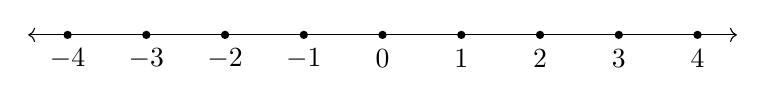
\begin{tikzpicture}
                \draw[<->] (-4.5, 0) -- (4.5, 0);
    
                \foreach \x in {-4, -3, -2, -1, 0, 1, 2, 3, 4}
                    \fill (\x, 0) circle (1.5pt);

                \foreach \x in {-4, -3, -2, -1, 0, 1, 2, 3, 4}
                    \node at (\x, -0.3) {$\x$};
            \end{tikzpicture}
        \end{center}
        Moreover, note that $-1 = e^{-2\pi i/2}$ and $i = e^{2\pi i/4}$. Then the fibers of these elements are just the integral differences of $1/2, 1/4$, and $2/3$ respectively, since $4\pi i/3 = 2/3(2\pi i)$:
        \begin{align*}
            \phi\inv(-1) & = \frac 12 + \z = \set*{\left.\frac 12 + n~\right|~n \in \z} \\
            \phi\inv(i) & = \frac 14 + \z = \set*{\left.\frac 14 + n~\right|~n \in \z} \\
            \phi\inv(e^{4\pi i/3}) & = \frac 23 + \z = \set*{\left.\frac 23 + n~\right|~n \in \z} \qh
        \end{align*}
    \end{sol}
    \item Repeat the preceding exercise with the map $\varphi$ replaced by the map $\varphi : r \mapsto e^{4\pi i r}$.
    \begin{sol}
        The kernel of $\phi$ is $\frac12\z$, or
        \begin{center}
            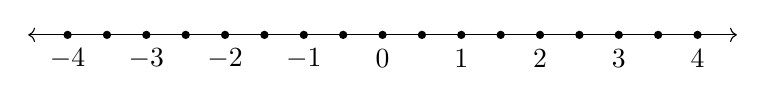
\begin{tikzpicture}
                \draw[<->] (-4.5, 0) -- (4.5, 0);
    
                \foreach \x in {-4, -3.5, -3, -2.5, -2, -1.5, -1, -0.5, 0, 0.5, 1, 1.5, 2, 2.5, 3, 3.5, 4}
                    \fill (\x, 0) circle (1.5pt);

                \foreach \x in {-4, -3, -2, -1, 0, 1, 2, 3, 4}
                    \node at (\x, -0.3) {$\x$};
            \end{tikzpicture}
        \end{center}
        Moreover, the fibers are just all halved, so
        \begin{align*}
            \phi\inv(-1) & = \frac14 + \frac12 \z = \set*{\left.\frac14 + \frac n2~\right|~n \in \z} \\
            \phi\inv(-i) & = \frac18 + \frac12 \z = \set*{\left.\frac18 + \frac n2~\right|~n \in \z} \\
            \phi\inv(e^{4\pi i/3}) & = \frac13 + \frac12 \z = \set*{\left.\frac13 + \frac n2~\right|~n \in \z} \qh
        \end{align*}
    \end{sol}
    \item Consider the additive quotient group $\mathbb{Q}/\mathbb{Z}$.
    \begin{problems}
        \item Show that every coset of $\mathbb{Z}$ in $\mathbb{Q}$ contains exactly one representative $q \in \mathbb{Q}$ in the range $0 \le q < 1$.
        \item Show that every element of $\mathbb{Q}/\mathbb{Z}$ has finite order but that there are elements of arbitrarily large order.
        \item Show that $\mathbb{Q}/\mathbb{Z}$ is the torsion subgroup of $\mathbb{R}/\mathbb{Z}$ (cf.\ Exercise 6, Section 2.1).
        \item Prove that $\mathbb{Q}/\mathbb{Z}$ is isomorphic to the multiplicative group of roots of unity in $\mathbb{C}^\times$.
    \end{problems}
    \begin{solalph}
        \item Suppose $t \in \q$, and put $t = a/b$ in lowest terms. Then there exists unique $q, r$ such that $a = bq + r$, or that $t = q + r/b$, where $0 \leq r < 1$. Then $t + \z = q + r/b + \z = r/b + \z$. Since $r$ is unique, then $r/b$ is the representative of $t + \z$ such that $0 \leq r < 1$.
        \item Suppose $t = p/q \in \q$. Then $|t + \z| \leq q$, since $q(t + \z) = qt + \z = \z$ so that $t + \z$ has finite order. Moreover, $1/k + \z \in \q/\z$ has order $k$, but because $k \in \z$ can be made arbitrarily large, then $1/k + \z$ has arbitrarily large order.
        \item Note that $\q/\z \subseteq \tor(\r/\z)$ by the previous exercise, so it remains to show that cosets with irrational representatives do not have finite order. If $x + \z \in \r/\z$ with finite order $n$, and $x \in \r - \q$, then $n(x + \z) = nx + \z = \z$ implies that $nx \in \z$. But since $n \in \zp$, this implies that $x \in \z$, contradicting that it was irrational. Hence, $\tor(\r/\z) = \q/\z$.
        \item By Exercise 3.1.12, we have $\r/\z \cong S^1$. Note that $\tor(S^1)$ consists of $z \in \c\unt$ such that $z^n = 1$, which is precisely the set of roots of unity. Since $\tor(\r/\z) = \q/\z$, then $\q/\z$ is isomorphic to the set of roots of unity.
    \end{solalph}
    \item Prove that a quotient of a divisible abelian group by any proper subgroup is also divisible. Deduce that $\mathbb{Q}/\mathbb{Z}$ is divisible (cf.\ Exercise 19, Section 2.4).
    \begin{sol}
        Let $A$ be a divisible abelian group, and let $B$ be a proper subgroup of $A$. Pick $aB \in A/B$. Since $A$ is divisible, there exists $x \in A$ such that $x^n = a$ for $x \in A$ and $n \in \z$. Then $(xB)^n = x^nB = aB$ so that $A/B$ is divisible. Since $\q$ is divisible, and $\z < \q$ is proper, then $\q/\z$ is also divisible.
    \end{sol}
    \item Let $G$ be a group, let $N$ be a normal subgroup of $G$, and let $\bar{G} = G/N$. Prove that if $G = \langle x, y \rangle$ then $\bar{G} = \langle \bar{x}, \bar{y} \rangle$. Prove more generally that if $G = \langle S \rangle$ for any subset $S$ of $G$, then $\bar{G} = \langle \bar{S} \rangle$.
    \begin{sol}
        If $G = \gen S$, then for every $g \in G$, we have
        \[g = s_1s_2 \dots s_n \quad \text{where $s_i \in S$ for $1 \le i \le n$}\]
        Let $\bar S = \{sN \mid s \in S\}$. Then for any $\bar g \in \bar G$, we have
        \[gN = (s_1s_2 \ldots s_n)N = (s_1N)(s_2N) \dots (s_nN)\]
        so that $\bar g \in \bar S$. Hence, $\bar G = \gen{\bar S}$. The case where $\bar G = \gen{\bar x, \bar y}$ is similar, where every element $g \in G$ is of the form $g = w(x, y)$, where $w(x, y)$ denotes a word in $\gen{x, y}$.
    \end{sol}
    \item Let $G$ be the dihedral group of order $16$ (whose lattice appears in Section 2.5): $G = \langle r,s \mid r^8 = s^2 = 1,\ rs = sr^{-1} \rangle$, and let $\bar{G} = G/\langle r^4 \rangle$ be the quotient of $G$ by the subgroup generated by $r^4$ (this subgroup is the center of $G$, hence is normal).
    \begin{problems}
        \item Show that the order of $\bar{G}$ is $8$.
        \item Exhibit each element of $\bar{G}$ in the form $\bar{s}^a \bar{r}^b$, for some integers $a$ and $b$.
        \item Find the order of each of the elements of $\bar{G}$ exhibited in (b).
        \item Write each of the following elements of $\bar{G}$ in the form $\bar{s}^a \bar{r}^b$, for some integers $a$ and $b$ as in (b): $\bar{rs}$, $\bar{sr^{-2}s}$, $\bar{s^{-1}r^{-1}sr}$.
        \item Prove that $\bar{H} = \langle \bar{s}, \bar{r}^2 \rangle$ is a normal subgroup of $\bar{G}$ and $\bar{H}$ is isomorphic to the Klein $4$-group. Describe the isomorphism type of the complete preimage of $\bar{H}$ in $G$.
        \item Find the center of $\bar G$ and describe the isomorphism type of $\bar G/Z(\bar G)$.
    \end{problems}
    \begin{solalph}
        \item Since $\gen{r^4} = \set{1, r^4}$, each coset in $\bar G$ has 2 elements and partitions $G$ into 8 sets. Hence, $\abs{\bar G} = 8$.
        \item The elements of $\bar G$ are
        \begin{align*}
            \bar 1 & = \{1, r^4\}, & \bar{s} & = \{s, sr^4\} \\
            \bar r & = \{r, r^5\}, & \bar{sr} & = \{sr, sr^5\} \\
            \bar r^2 & = \{r^2, r^6\}, & \bar{sr^2} & = \{sr^2, sr^6\} \\
            \bar r^3 & = \{r^3, r^7\}, & \bar{sr^3} & = \{sr^3, sr^7\}
        \end{align*}
        \item The orders of the elements of $\bar G$ are
        \[
        \begin{array}{c|c|c|c|c|c|c|c|c}
            \bar x & \bar 1 & \bar r & \bar r^2 & \bar r^3 & \bar s & \bar{sr} & \bar{sr^2} & \bar{sr^3} \\
            \hline
            \abs x & 1 & 4 & 2 & 4 & 2 & 2 & 2 & 2
        \end{array}
        \]
        \item $\bar{rs} = \bar{sr^3}, \bar{sr^{-2}s} = \bar r^2, \bar{s\inv r\inv sr} = \bar r^2$.
        \item We first note that $\bar H = \{1, \bar r^2, \bar s, \bar{sr^2}\}$. To show that $\bar H \nsub \bar G$, we simplify the process by noting that elements of $\bar G$ are of the form $\bar r^k$ or $\bar{sr^k}$. If an element is of the former, we have
        \begin{align*}
            \bar{r^kr^2r^{-k}} = \bar r^2 \in \bar H \\
            \bar{r^ksr^{-k}} = \bar{s(r^2)^{-k}} \in \bar H
        \end{align*}
        If it is of the latter, then
        \begin{align*}
            \bar{(sr^k)r^2(r^{-k}s)} = \bar{r^{-2}} \in H \\
            \bar{(sr^k)s(r^{-k}s)} = \bar{s(r^2)^k} \in H
        \end{align*}
        where $\bar{sr^k}\inv = \bar{r^{-k}s}$. The above calculations show that for every $\bar g \in \bar G$, then $\bar{gr^2g\inv}, \bar{gsg\inv} \in H$ so that $\bar{gHg\inv} = \bar H$, hence $\bar H \nsub \bar G$. Moreover, it is easy to see that every element of $\bar H$ is of order 2 so that $\bar H \cong V_4$.

        Let $\pi : G \to \bar G$ be the natural projection of $G$ onto $\bar G$. Then $\pi\inv(\bar H)$ is the complete preimage of $\bar H$, or the set of elements that map to a coset in $\bar H$. Using part (b), we see that
        \[\pi\inv(\bar H) = \{1, r^2, r^4, r^6, s, sr^2, sr^4, sr^6\}\]
        Note that $|\pi\inv(\bar H)| = 8$, and the elements of $\bar H$ satisfy the relations $(r^2)^4 = s^2 = 1$. Then the mapping $\phi : D_8 \to \pi\inv(\bar H)$ given by $\phi(r) = r^2$ and $\phi(s) = s$ extends to a homomorphism that is clearly surjective. Then $\phi$ is an isomorphism, and $\pi\inv(\bar H) \cong D_8$.
        \item From the previous exercise, we have that $\bar G = \gen{\bar r, \bar s}$. Since $\bar r^2$ commutes with both $\bar r$ and $\bar s$, then $\bar r^2 \in Z(\bar G)$. However, $\bar{rs} \neq \bar{sr}$ and $\bar{r^3s} \neq \bar{sr^3}$. Additionally, none of $\bar{sr}, \bar{sr^2}$, nor $\bar{sr^3}$ commute with $\bar r$ so that $Z(\bar G) = \{\bar 1, \bar r^2\}$. The elements of $\widehat G = \bar G/Z(\bar G)$ are as follows:
        \begin{align*}
            \hat 1 & = \{\bar 1, \bar r^2\} & \hat s & = \{\bar s, \bar{sr^2}\} \\
            \hat r & = \{\bar r, \bar r^3\} & \widehat{sr} & = \{\bar{sr}, \bar{sr^3}\}
        \end{align*}
        One can see that each nonidentity element of $\widehat G$ has order 2 so that $\widehat G \cong V_4$.
    \end{solalph}
    \item Let $G$ be the quasidihedral group of order $16$ (whose lattice was computed in Exercise 11 of Section 2.5): $G = \langle \sigma,\tau \mid \sigma^8 = \tau^2 = 1,\ \sigma\tau = \tau\sigma^3 \rangle$, and let $\bar{G} = G/\langle \sigma^4 \rangle$ be the quotient of $G$ by the subgroup generated by $\sigma^4$ (this subgroup is the center of $G$, hence is normal).
    \begin{problems}
        \item Show that the order of $\bar{G}$ is $8$.
        \item Exhibit each element of $\bar{G}$ in the form $\bar{\tau}^a \bar{\sigma}^b$, for some integers $a$ and $b$.
        \item Find the order of each of the elements of $\bar{G}$ exhibited in (b).
        \item Write each of the following elements of $\bar{G}$ in the form $\bar{\tau}^a \bar{\sigma}^b$, for some integers $a$ and $b$ as in (b): $\bar{\sigma\tau}$, $\bar{\tau\sigma^{-2}\tau}$, $\bar{\tau^{-1}\sigma^{-1}\tau\sigma}$.
        \item Prove that $\bar{G} \cong D_8$.
    \end{problems}
    \begin{solalph}
        \item $\gen{\sigma^4}$ has 2 elements, so each coset has 2 elements which subsequently split $G$ into 8 cosets. Hence, $\abs{\bar G} = 8$.
        \item The elements are
        \begin{align*}
            \bar 1 & = \{1, \sigma^4\} & \bar\tau & = \{\tau, \tau\sigma^4\} \\
            \bar\sigma & = \{\sigma, \sigma^5\} & \bar{\tau\sigma} & = \{\tau\sigma, \tau\sigma^5\} \\
            \bar\sigma^2 & = \{\sigma^2, \sigma^6\} & \bar{\tau\sigma^2} & = \{\tau\sigma^2, \tau\sigma^6\} \\
            \bar\sigma^3 & = \{\sigma^3, \sigma^7\} & \bar{\tau\sigma^3} & = \{\tau\sigma^3, \tau\sigma^7\}
        \end{align*}
        \item The orders are
        \[
        \begin{array}{c|c|c|c|c|c|c|c|c}
            \bar x & \bar 1 & \bar\sigma & \bar\sigma^2 & \bar\sigma^3 & \bar\tau & \bar{\tau\sigma} & \bar{\tau\sigma^2} & \bar{\tau\sigma^3} \\
            \hline
            \abs{\bar x} & 1 & 4 & 2 & 4 & 2 & 2 & 2 & 2
        \end{array}
        \]
        \item $\bar{\sigma\tau} = \bar{\tau\sigma^3}, \bar{\tau\sigma^{-2}\tau} = \bar\sigma^2, \bar{\tau\inv\sigma\inv\tau\sigma} = \bar\sigma^2$.
        \item Note that $\bar\sigma^4 = \bar\tau^2 = \bar 1$, and $\bar{\sigma\tau} = \bar{\tau\sigma^3} = \bar{\tau\sigma^7} = \bar{\tau\sigma}$ so that $\bar G$ satisfies the same relations in $D_8$. Then the mapping $\phi : \bar G \to D_8$ given by $\phi(\bar\sigma) = r$ and $\phi(\bar\tau) = s$ extends to a surjective homomorphism, hence $\bar G \cong D_8$.
    \end{solalph}
    \item Let $G$ be the modular group of order $16$ (whose lattice was computed in Exercise 14 of Section 2.5): $G = \langle u,v \mid u^2 = v^8 = 1,\ vu = uv^5 \rangle$, and let $\bar{G} = G/\langle v^4 \rangle$ be the quotient of $G$ by the subgroup generated by $v^4$ (this subgroup is contained in the center of $G$, hence is normal).
    \begin{problems}
        \item Show that the order of $\bar{G}$ is $8$.
        \item Exhibit each element of $\bar{G}$ in the form $\bar{u}^a \bar{v}^b$, for some integers $a$ and $b$.
        \item Find the order of each of the elements of $\bar{G}$ exhibited in (b).
        \item Write each of the following elements of $\bar{G}$ in the form $\bar{u}^a \bar{v}^b$, for some integers $a$ and $b$ as in (b): $\bar{vu}$, $\bar{uv^{-2}u}$, $\bar{u^{-1}v^{-1}uv}$.
        \item Prove that $\bar{G}$ is abelian and is isomorphic to $Z_2 \times Z_4$.
    \end{problems}
    \begin{solalph}
        \item $\gen{v^4}$ has 2 elements, so each coset has 2 elements. Then $G$ is split into 8 cosets, hence $\abs{\bar G} = 8$.
        \item The elements are
        \begin{align*}
            \bar 1 & = \{1, v^4\} & \bar u & = \{u, uv^4\} \\
            \bar v & = \set{v, v^5} & \bar{uv} & = \set{uv, uv^5} \\
            \bar v^2 & = \set{v^2, v^6} & \bar{uv^2} & = \set{uv^2, uv^6} \\
            \bar v^3 & = \set{v^3, v^7} & \bar{uv^3} & = \set{uv^3, uv^7}
        \end{align*}
        \item The orders are
        \[
        \begin{array}{c|c|c|c|c|c|c|c|c}
            \bar x & \bar 1 & \bar v & \bar v^2 & \bar v^3 & \bar u & \bar{uv} & \bar{uv^2} & \bar{uv^3} \\
            \hline
            \abs{\bar x} & 1 & 4 & 2 & 4 & 2 & 2 & 2 & 2
        \end{array}
        \]
        \item $\bar{vu} = \bar{uv^5}, \bar{uv^{-2}u} = \bar u^2, \bar{u\inv v\inv uv} = \bar 1$.
        \item Since $\bar{vu} = \bar{uv^5} = \bar{uv}$, $\bar G$ is abelian. Moreover, using the presentation of $Z_2 \times Z_4$ in \hyperref[ex2.5.12]{Section 2.5, Exercise 12}, we see that $\bar u^2 = \bar v^4 = 1$ so that $\bar G$ satisfies the same relations. Then $\phi : \bar G \to Z_2 \times Z_4$ given by $\phi(\bar u) = a$ and $\phi(\bar v) = b$ is a surjective homomorphism, hence $\bar G \cong Z_2 \times Z_4$.
    \end{solalph}
    \item Let $G = \mathbb{Z}/24\mathbb{Z}$ and let $\wt{G} = G/\langle \bar{12} \rangle$, where for each integer $a$ we simplify notation by writing $\wt{\bar a}$ as $\wt{a}$.
    \begin{problems}
        \item Show that $\wt{G} = \{ \wt{0}, \wt{1}, \ldots, \wt{11} \}$.
        \item Find the order of each element of $\bar{G}$.
        \item Prove that $\wt{G} \cong \mathbb{Z}/12\mathbb{Z}$ (thus $(\mathbb{Z}/24\mathbb{Z})/(12\mathbb{Z}/24\mathbb{Z}) \cong \mathbb{Z}/12\mathbb{Z}$, just as if we inverted and canceled the $24\mathbb{Z}$'s).
    \end{problems}
    \begin{solalph}
        \item Note that for some $\wt x \in \wt G$, we have $\wt x = \bar x\gen{12} = \{\bar x, \bar{x + 12}\}$. It follows that $x = 0, 1, 2, \dots, 11$ produces distinct cosets.
        \item The orders are
        \[
        \begin{array}{c|c|c|c|c|c|c|c|c|c|c|c|c}
            \wt x & \wt 0 & \wt 1 & \wt 2 & \wt 3 & \wt 4 & \wt 5 & \wt 6 & \wt 7 & \wt 8 & \wt 9 & \wt{10} & \wt{11} \\
            \hline
            \abs{\wt x} & 1 & 12 & 6 & 4 & 3 & 12 & 2 & 12 & 3 & 4 & 6 & 12
        \end{array}
        \]
        \item Define the mapping $\phi : \wt G \to \intmod[12]$ given by $\phi(\wt x) = \bar x$. This map is trivially a bijection, and for any $\wt x, \wt y \in \wt G$, then
        \[\phi(\wt x + \wt y) = \phi(\wt{x + y}) = \bar{x + y} = \bar x + \bar y = \phi(\wt x) + \phi(\wt y)\]
        so that $\phi$ is a homomorphism. Then $\wt G \cong \intmod[12]$.
    \end{solalph}
    \item Let $G = Z_4 \times Z_4$ be given in terms of the following generators and relations:
    \[G = \gen{x, y \mid x^4 = y^4 = 1, xy = yx}\]
    Let $\bar G = G/\gen{x^2y^2}$ (note that every subgroup of the abelian group $G$ is normal).
    \begin{problems}
        \item Show that the order of $\bar G$ is 8.
        \item Exhibit each element of $\bar G$ in the form $\bar x^a \bar y^b$ for some integers $a$ and $b$.
        \item Find the order of each elements of $\bar G$ exhibited in (b).
        \item Prove that $\bar G \cong Z_4 \times Z_2$.
    \end{problems}
    \begin{solalph}
        \item Note that $(x^2y^2)^2 = x^4y^4 = 1$ so that $\gen{x^2y^2} = \{1, x^2y^2\}$. Then each coset of $\bar G$ has 2 elements, hence its order is 8.
        \item Noting that $\bar x^2 \bar y^2 = \bar 1$ in $\bar G$, we have $\bar x^2 = \bar y^2$. Then we have the elements
        \begin{align*}
            \bar 1 & = \{1, x^2y^2\} & \bar y & = \{y, x^2y^3\} \\
            \bar x & = \{x, x^3y^2\} & \bar{xy} & = \{xy, x^3y^3\} \\
            \bar x^2 & = \{x^2, y^2\} & \bar{x^2y} & = \{x^2y, y^3\} \\
            \bar x^3 & = \{x^3, xy^2\} & \bar{x^3y} & = \{x^3y, xy^3\}
        \end{align*}
        \item The orders are
        \[
        \begin{array}{c|c|c|c|c|c|c|c|c}
            \bar g & \bar 1 & \bar x & \bar x^2 & \bar x^3 & \bar y & \bar{xy} & \bar{x^2y} & \bar{x^3y} \\
            \hline
            \abs{\bar g} & 1 & 4 & 2 & 4 & 4 & 2 & 4 & 2
        \end{array}
        \]
        \item Using the presentation of $Z_2 \times Z_4$ in \hyperref[ex2.5.12]{Section 2.5, Exercise 12}, and noting that $\bar{xy}^2 = \bar x^4 = 1$ then the mapping $\phi : Z_2 \times Z_4 \to \bar G$ given by
        \[\phi(a) = \bar{xy}, \quad \phi(b) = \bar x\]
        extends to a unique homomorphism. Now suppose $\phi(a^sb^t) = \phi(a^ub^v)$. Then $\bar{xy}^s\bar x^t = \bar{xy}^u\bar x^v$. Since $\gen{\bar{xy}} \cap \gen{\bar x}$ is trivial, then $\bar{xy}^{s - u} = \bar x^{v - t}$ imply that both quantities must be one. Then $\bar{xy}^s = \bar{xy}^u$ and $\bar x^v = \bar x^t$. Then $s \equiv u \bmod 2$ and $v \equiv t \bmod 4$, so that $a^sb^t = a^ub^t$ since $\abs a = 2$ and $\abs b = 4$. Then $\phi$ is injective. Because $\abs{Z_2 \times Z_4} = \abs{\bar G} = 8$, then $\phi$ is an isomorphism, hence $\bar G \cong Z_2 \times Z_4 \cong Z_4 \times Z_2$.
    \end{solalph}
    \item
    \begin{problems}
        \item Prove that if $H$ and $K$ are normal subgroups of a group $G$ then their intersection $H \cap K$ is also a normal subgroup of $G$.
        \item Prove that the intersection of an arbitrary nonempty collection of normal subgroups of a group is a normal subgroup (do not assume the collection is countable).
    \end{problems}
    \begin{solalph}
        \item Observe that $H \cap K \leq G$ since $H \leq G$ and $K \leq G$. Let $g \in G$ and $x \in H \cap K$. Since $H \nsub G$ and $K \nsub G$, then $gxg\inv \in H$ and $gxg\inv \in K$, hence $gxg\inv \in H \cap K$. Then $g(H \cap K)g\inv \subseteq H \cap K$. By \autoref{theo3.6}, then $H \cap K \nsub G$.
        \item Let $G$ be a group and $I$ be a nonempty set of indices, possibly not countable. Consider the collection of subgroups $\{N_i \mid i \in I\}$ of $G$, where $N_i \nsub G$ for every $i \in I$. Consider their intersection
        \[N = \bigcap_{i \in I} N_i\]
        Since $N \leq G$, what remains to be shown is that $gNg\inv \subseteq N$ for some $g \in G$. To that end, let $n \in N$. Then $gng\inv \in N_i$ for each $i \in I$ because $N_i \nsub G$. It follows that $gng\inv \in N$ so that $gNg\inv \subseteq N$.
    \end{solalph}
    \item Prove that the join (cf. Section 2.5) of any nonempty collection of normal subgroups of a group is a normal subgroup.
    \begin{sol}
        Let $G$ be a group and $I$ be a nonempty set of indices. Let $\{N_i \mid i \in I\}$ be a collection of normal subgroups of $G$, and let $N = \gen{N_i \mid i \in I}$ be the join of the collection. Let $g \in G$ and $n \in N$. Then
        \[n = n_1n_2 \dots n_k \quad \text{where $n_i \in N_i$ for some $i \in I$}\]
        Since $N_i \nsub G$, then $gn_ig\inv \in N_i$ for each $1 \leq i \leq k$. Then
        \[gng\inv = g(n_1n_2 \ldots n_k)g\inv = (gn_1g\inv)(gn_2g\inv) \cdots (gn_kg\inv)\]
        Because $gng\inv$ is written as a product of elements where each one belongs to some $N_i$, it follows that it is in the join $N$, hence $gNg\inv \subseteq N$. Then $N \nsub G$.
    \end{sol}
    \item Prove that if $N \nsub G$ and $H$ is any subgroup of $G$ then $N \cap H \nsub H$.
    \begin{sol}
        We know $N \cap H \leq G$, so pick $h \in H$ and $x \in N \cap H$. Since $N \nsub G$, then $hxh\inv \in N$. Since $H \leq G$, then $hxh\inv \in H$ so that $hxh\inv \in N \cap H$. Then $N \cap H \nsub H$.
    \end{sol}
    \item 
    \begin{problems}
        \item Prove that a subgroup $N$ of $G$ is normal if and only if $gNg^{-1} \subseteq N$ for all $g \in G$.
        \item Let $G = \gl_2(\mathbb{Q})$, let $N$ be the subgroup of upper triangular matrices with integer entries and $1$'s on the diagonal, and let $g$ be the diagonal matrix with entries $2,1$. Show that $gNg^{-1} \subseteq N$ but $g$ does not normalize $N$.
    \end{problems}
    \begin{solalph}
        \item \rightimp If $N \nsub G$, then $gNg\inv \subseteq N$ holds true for all $g \in G$.
        \down\noindent
        \leftimp Suppose $gNg\inv \subseteq N$ for every $g \in G$, and let $n \in N$. To show that $N \subseteq gNg\inv$, note for some $g \in G$, then $g\inv Ng \subseteq N$ so that $g\inv ng \in N$. It follows that $n = g(g\inv ng)g\inv \in gNg\inv$ so that $N = gNg\inv$, hence $N \nsub G$.
        \item Let
        \[n = 
        \begin{pmatrix}
            1 & x \\
            0 & 1
        \end{pmatrix} \in N\]
        where $x \in \z$. Then
        \[gng\inv = 
        \begin{pmatrix}
            2 & 0 \\
            0 & 1
        \end{pmatrix}
        \begin{pmatrix}
            1 & x \\
            0 & 1
        \end{pmatrix}
        \begin{pmatrix}
            1/2 & 0 \\
            0 & 1
        \end{pmatrix} = 
        \begin{pmatrix}
            1 & 2x \\
            0 & 1
        \end{pmatrix} \in N\]
        since $2x \in \z$. Notice that the upper right entry of $gng\inv$ for any $n \in N$ will be even, so any matrix with an odd integer in the upper right entry will have no such $n \in N$ such that $gng\inv$ is that matrix.
    \end{solalph}
    \item Let $a,b \in G$.
    \begin{problems}
        \item Prove that the conjugate of the product of $a$ and $b$ is the product of the conjugate of $a$ and the conjugate of $b$. Prove that the order of $a$ and the order of any conjugate of $a$ are the same.
        \item Prove that the conjugate of $a^{-1}$ is the inverse of the conjugate of $a$.
        \item Let $N = \langle S \rangle$ for some subset $S$ of $G$. Prove that $N \nsub G$ if $gSg^{-1} \subseteq N$ for all $g \in G$.
        \item Deduce that if $N$ is the cyclic group $\langle x \rangle$, then $N$ is normal in $G$ if and only if for each $g \in G$, $gxg^{-1} = x^k$ for some $k \in \mathbb{Z}$.
        \item Let $n$ be a positive integer. Prove that the subgroup $N$ of $G$ generated by all the elements of $G$ of order $n$ is a normal subgroup of $G$.
    \end{problems}
    \begin{solalph}
        \item Note that $g(ab)g\inv = (gag\inv)(gbg\inv)$. The second result follows by \hyperref[ex1.1.22]{Exercise 1.1.22}.
        \item For any $g \in G$, then
        \[(ga\inv g\inv)(gag\inv) = ga\inv (g\inv g) ag\inv = g(a\inv a)g\inv = gg\inv = 1\]
        so that $(gag\inv)\inv = ga\inv g\inv$.
        \item If $S$ is empty, then $N$ is trivial, so the result follows. Suppose $S$ is not empty, and pick $n \in N$. Because $N = \gen S$, then we have $n = s_1s_2 \ldots s_k$, where $s_i \in S$ for each $i = 1, 2, \ldots, k$. Since 
        \[gng\inv = (gs_1g\inv)(gs_2g\inv) \cdots (gs_kg\inv)\]
        for every $g \in G$, and $gSg\inv \subseteq N$, then the right hand side is also in $N$, hence $gNg\inv \subseteq N$ so that $N \nsub G$.
        \item \rightimp Immediate from the definition of a normal subgroup.
        
        \noindent \leftimp Put $S = \set x$ and use the previous part.
        \item Let $S = \set{g \in G \mid \abs g = n}$, and put $N = \gen S$. If $S$ is empty, then $N$ is trivial, hence is normal. If $S$ is nonempty, note that part (a) shows that for any $g \in G$ and $s \in S$, then $\abs{gsg\inv} = \abs s = n$ so that $gsg\inv \in S \subseteq N$. Then $gSg\inv \subseteq N$, hence $N \nsub G$ by part (c).
    \end{solalph}
    \item Let $N$ be a \textit{finite} subgroup of a group $G$. Show that $gNg^{-1} \subseteq N$ if and only if $gNg^{-1} = N$. Deduce that $N_G(N) = \{ g \in G \mid gNg^{-1} \subseteq N \}$.
    \begin{sol}
        \rightimp Suppose $gNg\inv \subseteq N$. For any $g \in G$, define a mapping $\phi : N \to gNg\inv$ given by $\phi(n) = gng\inv$. If $\phi(m) = \phi(n)$, then $gmg\inv = gng\inv$ so that $\phi$ is injective by cancellation. Moreover, if $m \in gNg\inv$, there exists $n \in N$ such that $m = gng\inv = \phi(n)$ so that $\phi$ is surjective. It follows that $\phi$ is a bijection, and $\abs N = \abs{gNg\inv}$. Since $gNg\inv \subseteq N$, and $N$ is finite, it follows that $gNg\inv = N$.

        \noindent \leftimp Immediate.

        Note that $N_G(N) = \set{g \in G \mid gNg\inv = N}$. We may replace the condition that $gNg\inv = N$ with $gNg\inv \subseteq N$ by the implication showed above.
    \end{sol}
    \item Let $N$ be a \textit{finite} subgroup of a group $G$ and assume $N = \langle S \rangle$ for some subset $S$ of $G$. Prove that an element $g \in G$ normalizes $N$ if and only if $gSg^{-1} \subseteq N$.
    \begin{sol}
        \rightimp Immediate, since $gSg\inv \subseteq gNg\inv = N$ because $g \in N_G(N)$.

        \noindent \leftimp If $S$ is empty, then $N$ is trivial hence the conclusion follows. Suppose $S$ is not empty, and pick $n \in N$. Then $n = s_1s_2 \dots s_k$, where $s_i \in S$ for every $i = 1, 2, \ldots, k$. Then $gng\inv = gs_1g\inv gs_2g\inv \ldots gs_kg\inv \in N$ because $gs_ig\inv \in gSg\inv \subseteq N$. Then $gNg\inv \subseteq N$, and by the previous exercise, $g \in N_G(N)$. 
    \end{sol}
    \item Let $N$ be a \textit{finite} subgroup of $G$ and suppose $G = \langle T \rangle$ and $N = \langle S \rangle$ for some subsets $S$ and $T$ of $G$. Prove that $N$ is normal in $G$ if and only if $tSt^{-1} \subseteq N$ for all $t \in T$.
    \begin{sol}
        \rightimp Immediate, since $gNg\inv = N$ for every $g \in G$, so $tSt\inv \subseteq N$.

        \noindent \leftimp Suppose $S$ and $T$ are nonempty subsets of $G$, and let $g \in G$. Since $g \in \gen T$, then $g = t_1t_2 \dots t_k$, where $t_i \in T$ for each $i = 1, 2, \ldots, k$. Since we need to show this for every $g \in G$, we must proceed by inducting on the word length of $g \in \gen T$. To that end, $t_1St_1\inv \subseteq N$, so the base case is satisfied. Assume now that $gSg\inv \subseteq N$ when $g$ is some $k$-length word made up of elements from $T$. Consider the $k+1$-length word $g = t_1t_2 \ldots t_kt_{k + 1}$, where $t_i \in T$ for each $i = 1, 2, \ldots, k + 1$. For notation, set $\hat t = t_1t_2 \ldots t_k$ so that $g = \hat tt_{k + 1}$. The induction assumption shows that $\hat tS\hat t\inv \subseteq N$. For any $s \in S$, then 
        \[gsg\inv = \hat tt_{k + 1}st_{k + 1}\inv h\inv = \hat t(t_{k + 1}st_{k + 1}\inv)\hat t\inv\]
        where $t_{k + 1}st_{k + 1}\inv \in N$ because $tSt\inv \subseteq N$ for every $t \in T$. Since $N = \gen S$, then we may set $t_{k + 1}st_{k + 1}\inv = s_1s_2 \ldots s_m$, where $s_i \in S$ for every $i = 1, 2, \ldots, m$. Then
        \[\hat t(t_{k + 1}st_{k + 1}\inv)\hat t\inv = (\hat ts_1\hat t\inv)(\hat ts_2 \hat t\inv) \cdots (\hat ts_m \hat t\inv) \in N\]
        Hence, $gsg\inv \in N$ so that $gSg\inv \subseteq N$. Induction shows that this is true for every $g \in G$, and by finiteness of $N$, we use the result from the previous exercise to conclude that $N \nsub G$.
    \end{sol}
    \item Let $N \le G$ and let $g \in G$. Prove that $gN = Ng$ if and only if $g \in N_G(N)$.
    \begin{sol}
        \rightimp Suppose $gN = Ng$. For some $n \in N$, there exists $n' \in N$ such that $ng = gn'$, or $n = gn'g\inv$. Then $n \in gNg\inv$ so that $N \subseteq gNg\inv$. Moreover, if $n \in N$, then for some $n' \in N$ we have $gn = n'g$ so that $gng\inv = n'$, hence $gNg\inv \subseteq N$, hence $g \in N_G(N)$.
        
        \noindent \leftimp Suppose $g \in N_G(N)$ and $n \in N$. Since $n \in gNg\inv$, there exists $n' \in N$ such that $n = gn'g\inv$ so that $ng = gn'$, hence $n \in gN$, and $Ng \subseteq gN$. By symmetry, we have $gN \subseteq Ng$, hence $gN = Ng$.
    \end{sol}
    \item Prove that if $H \le G$ and $N$ is a normal subgroup of $H$ then $H \le N_G(N)$. Deduce that $N_G(N)$ is the largest subgroup of $G$ in which $N$ is normal (i.e. is the join of all subgroups $H$ for which $N \nsub H$).
    \begin{sol}
        If $h \in H$, then $hNh\inv = N$ because $N \nsub H$, hence $h \in N_G(N)$. Because $N_G(N) \leq G$, then $H \subseteq N_G(N)$ implies $H \leq N_G(N)$. Moreover, since every subgroup such that $N$ is normal in is a subgroup of $N_G(N)$, then $N_G(N)$ is the largest subgroup in which $N$ is normal.
    \end{sol}
    \item Prove that every subgroup of $Q_8$ is normal. For each subgroup find the isomorphism type of its corresponding quotient. [You may use the lattice of subgroups for $Q_8$ in Section 2.5.]
    \begin{sol}
        By the lattice, the subgroups of $Q_8$ are 1, $\gen{-1}, \gen i, \gen j, \gen k$, and $Q_8$. It is clear that $Q_8/1 \cong Q_8$, and $Q_8/Q_8 \cong 1$. Now, the lattice shows that $\gen i, \gen j$, and $\gen k$ are all maximal subgroups, so their normalizers must either be themselves, or $Q_8$. Since $j\gen i (-j) = \gen i$, then $j \in N_{Q_8}(\gen i)$ so that $N_{Q_8}(\gen i) = Q_8$. We may similarly argue that $N_{Q_8}(\gen j) = N_{Q_8}(\gen k) = Q_8$. Moreover, $Z(Q_8) = \gen{-1}$, and every center of a group is normal. It follows that every subgroup of $Q_8$ is normal.
        
        Let us first examine $Q_8/\gen{-1} = \{\bar 1, \bar i, \bar j, \bar k\}$. Since $\bar i^2 = \bar{-1} = \bar 1$, then $\abs{\bar i} = 2$. We can argue that $\abs{\bar j} = \abs{\bar k} = 2$ so that $Q_8/\gen{-1} \cong V_4$. The quotient group $Q_8/\gen i = \{\bar 1, \bar j\}$ has order 2 so $Q_8/\gen i \cong Z_2$. By symmetry, $Q_8/\gen j \cong Q_8/\gen k \cong Z_2$.
    \end{sol}
    \item Find all normal subgroups of $D_8$ and for each of these find the isomorphism type of its corresponding quotient. [You may use the lattice of subgroups for $D_8$ in Section 2.5.]
    \begin{sol}
        Again, $D_8/1 \cong D_8$ and $D_8/D_8 \cong 1$. Examining the three maximal subgroups $\gen{s, r^2}, \gen r$, and $\gen{rs, r^2}$. observe the following:
        \begin{align*}
            r\gen{s, r^2}r\inv & = \{1, sr^2. r^2, s\} = \gen{s, r^2} \\
            s\gen r s\inv & = \{1, r^3, r^2, r\} = \gen r \\
            r\gen{rs, r^2}r\inv & = \{1, sr, r^2, sr^3\} = \gen{rs, r^2}
        \end{align*}
        so that the normalizers of each of the subgroups contain $r$ and $s$, hence $N_{D_8}(\gen{s, r^2}) = N_{D_8}(\gen r) = N_{D_8}(\gen{rs, r^2}) = Q_8$. Moreover, each of these maximal subgroups are of order 4, which means their corresponding quotient groups will have order 2, hence $Q_8/\gen{s, r^2} \cong Q_8/\gen r \cong Q_8/\gen{rs, r^2} \cong Z_2$.

        Now we examine $\gen{r^2} = Z(D_8)$ so it is clearly normal. Then $D_8/\gen{r^2} = \{\bar 1, \bar r, \bar s, \bar{sr}\}$. Note that the nonidentity elements have order 2, and so $D_8/\gen{r^2} \cong V_4$.

        For the remaining subgroups of order 2, observe that
        \begin{align*}
            r\gen{s}r\inv & = \{1, sr^2\} \neq \gen s \\
            r\gen{sr}r\inv & = \{1, rs\} \neq \gen{sr} \\
            r\gen{sr^2}r\inv & = \{1, s\} \neq \gen{sr^2} \\
            r\gen{sr^3}r\inv & = \{1, sr\} \neq \gen{sr^3}
        \end{align*}
        so that none of the subgroups of order 2 contain $r$, hence none of them are normal.
    \end{sol}
    \item Let $D_{2n} = \langle r,s \mid r^n = s^2 = 1,\ rs = sr^{-1} \rangle$ be the usual presentation of the dihedral group of order $2n$ and let $k$ be a positive integer dividing $n$.
    \begin{problems}
        \item Prove that $\langle r^k \rangle$ is a normal subgroup of $D_{2n}$.
        \item Prove that $D_{2n}/\langle r^k \rangle \cong D_{2k}$.
    \end{problems}
    \begin{solalph}
        \item Observe that $\gen{r^k} = \{1, r^k, r^{2k}, \ldots, r^{n - k}\}$. It is clear that $r\gen{r^k}r\inv = \gen{r^k}$, and observe that $sr^ks\inv = r^{-k} = r^{n - k}$ so that $s\gen{r^k}s\inv = \gen{r^k}$. Since $r, s \in N_{D_{2n}}(\gen{r^k})$, then $\gen{r^k} \nsub D_{2n}$.
        \item Consider $D_{2n}/\gen{r^k}$. Since $k \mid n$, then the order of $\gen{r^k}$ is $n/k$, and the number of cosets in the quotient group is $2n/(n/k) = 2k$. Now consider the cosets $\bar r$ and $\bar s$:
        \[\bar r = \{r, r^{k + 1}, r^{2k + 1}, \ldots, r^{n - k + 1}\} \quad \text{and} \quad \bar s = \{s, sr^k, sr^{2k}, \ldots, sr^{n - k}\}\]
        It is clear that $\bar s \neq \bar 1$, and $\bar s^2 = \bar 1$ so that $\abs{\bar s} = 2$. Moreover, $\bar r^k = \bar 1$, hence $\abs{\bar r} \leq k$. However, note that $\bar r^i = \bar 1$ when $i \mid k$ so that $\abs{\bar r} = k$. This clearly satisfies the relations for $D_{2k}$, hence $D_{2n}/\gen{r^k} \cong D_{2k}$. 
    \end{solalph}
    \item Prove that $\speclin_n(F) \nsub \gl_n(F)$ and describe the isomorphism type of the quotient group (cf. Exercise 9, Section 2.1).
    \begin{sol}
        We know that $\speclin_n(F) \leq \gl_n(F)$, so we just need to show that $A \speclin_n(F) A\inv = \speclin_n(F)$ for all $A \in \gl_n(F)$. To that end, note that for any $S \in \speclin_n(F)$ and $X \in \gl_n(F)$, we have $\det(XSX\inv) = \det(X)\det(S)\det(X\inv) = 1$, hence $X\speclin_n(F)X\inv \subseteq \speclin_n(F)$, and $\speclin_n(F) \nsub \gl_n(F)$.

        Recall that when a subgroup is normal, it is actually the kernel of some homomorphism. Observe that every element of $\speclin_n(F)$ has determinant 1, so if we consider the mapping $A \mapsto \det(A)$ for some $A \in \gl_n(F)$, then the kernel of this homomorphism is clearly $\speclin_n(F)$. We may then consider the mapping $\phi : \gl_n(F)/\speclin_n(F) \to F\unt$ given by $\phi(\bar X) = \det(X)$.

        We now show that this mapping is well defined. To that end, suppose $\bar A = \bar B$ for some $\bar A, \bar B \in \gl_n(F)/\speclin_n(F)$. Recall that the elements of $\bar A$ are of the form $AS$ for $A \in \gl_n(F)$ and some $S \in \speclin_n(F)$. Since $\bar A = \bar B$, then for $AS \in \bar A$ there exists $S' \in \speclin_n(F)$ such that $AS = BS_0$. Then
        \[\phi(\bar A) = \det(A) = \det(AS) = \det(BS') = \det(B) = \phi(\bar B)\]
        so that $\phi$ is well defined.
        
        To show that $\phi$ is injective, suppose $\phi(\bar A) = \phi(\bar B)$. Then $\det(A) = \det(B)$. Pick some $AS \in \bar A$, where $S \in \speclin_n(F)$. Observe that $B\inv AS \in \speclin_n(F)$, since $\det(B\inv AS) = \det(B\inv)\det(A)\det(S) = \det(A)\inv\det(A)\det(S) = 1$, hence $B\inv AS = S'$ for some $S' \in \speclin_n(F)$. Then $AS = BS'$, and $AS \in \bar B$ so that $\bar A \subseteq \bar B$. A similar argument shows that $\bar B \subseteq \bar A$ so that $\bar A = \bar B$, and $\phi$ is injective. Moreover, for some $f \in F\unt$, then $\det(fI_n) = f\det(I_n) = f$ so that $\phi$ is surjective. Lastly, for $\bar A, \bar B \in \speclin_n(F)$, then 
        \[\phi(\bar{AB}) = \det(AB) = \det(A)\det(B) = \phi(\bar A)\phi(\bar B)\]
        so that $\phi$ is a homomorphism. Then $\phi$ is a bijective homomorphism, and $\gl_n(F)/\speclin_n(F) \cong F\unt$. 
    \end{sol}
    \item Prove that if $G/Z(G)$ is cyclic then $G$ is abelian. [If $G/Z(G)$ is cyclic with generator $xZ(G)$, show that every element of $G$ can be written in the form $x^a z$ for some integer $a \in \mathbb{Z}$ and some element $z \in Z(G)$.]
    \begin{sol}
        Suppose $G/Z(G) = \gen{xZ(G)}$ for some $x \in G$. Then cosets are of the form $x^aZ(G)$ for some $a \in \z$. Suppose $g, h \in G$. Since both $g$ and $h$ belong to some coset in $G/Z(G)$, then $g = x^mz$ and $h = x^nz'$ for some $m, n \in \z$ and $z, z' \in Z(G)$. Then
        \[ab = (x^mz)(x^nz') = (x^nz')(x^mz) = ba\]
        so that $G$ is abelian.
    \end{sol}
    \item Let $A$ and $B$ be groups. Show that $\{(a,1) \mid a \in A\}$ is a normal subgroup of $A \times B$ and the quotient of $A \times B$ by this subgroup is isomorphic to $B$.
    \begin{sol}
        Let $C$ be the the given set. It is clear that $C \leq A \times B$. Suppose $(a, b) \in A \times B$. Then for any $(a', 1) \in C$, we have
        \[(a, b)(a', 1)(a, b)\inv = (aa'a\inv, b1b\inv) = (aa'a\inv, 1) \in C\]
        so that $C \nsub A \times B$.

        Consider the mapping $\phi : A \times B/C \to B$ given by $\phi(\bar{(a, b)}) = b$. To show that this is well-defined, suppose $\bar{(a, b)} = \bar{(a', b')}$. Then $(a, b)C = (a', b')C$, which implies that $C = (a\inv, b\inv)(a', b')C$, or that $(a\inv a', b\inv b') \in C$. Then $b\inv b' = 1$, or $b = b'$ so that $\phi$ is well-defined.

        Now suppose $\phi(\bar{(a, b)}) = \phi(\bar{(a', b')})$. Then $b = b'$ so that $(a, b)C = (a', b')C$, hence $\phi$ is injective. Moreover, $\phi(\bar{(1, b)}) = b$ so that $\phi$ is surjective. Lastly, for $\bar{(a, b)}, \bar{(a', b')} \in A \times B/C$, then 
        \[\phi(\bar{(a, b)}\bar{(a', b')}) = \phi(\bar{(aa', bb')}) = bb' = \phi(\bar{(a, b)})\phi(\bar{(a', b')})\]
        so that $\phi$ is a bijective homomorphism. Hence, $A \times B/C \cong B$.
    \end{sol}
    \item Let $A$ be an abelian group and let $D$ be the (diagonal) subgroup $\{(a,a) \mid a \in A\}$ of $A \times A$. Prove that $D$ is a normal subgroup of $A \times A$ and $(A \times A)/D \cong A$.
    \begin{sol}
        Since $A$ is abelian, then $A \times A$ is abelian, hence any subgroup is normal so that $D \nsub A \times A$.

        Now consider two cosets $\bar{(a_1, a_2)}, \bar{(a_3, a_4)} \in (A \times A)/D$. Then $\bar{(a_1, a_2)} = \bar{(a_3, a_4)}$ when $(a_1, a_2)\inv(a_3, a_4) \in D$, which implies that $a_1\inv a_3 = a_2\inv a_4$, or $a_3a_4\inv = a_1a_2\inv$. We can construct a well-defined, injective homomorphism $\phi : (A \times A)/D \to A$ given by $\phi(\bar{(a, b)}) = ab\inv$. Moreover, this is surective, since $\phi(\bar{(a, 1)}) = a$ for any $a \in A$. Lastly, it is a homomorphism, because
        \begin{align*}
            \phi(\bar{(a_1, b_1)(a_2, b_2)}) & = \phi(\bar{(a_1a_2, b_1b_2)}) \\
            & = (a_1a_2)(b_1b_2)\inv \\
            & = (a_1b_1\inv)(a_2b_2\inv) \\
            & = \phi(\bar{(a_1, b_1)})\phi(\bar{(a_2, b_2)})
        \end{align*}
        Hence, $\phi$ is a bijective homomorphism, and $(A \times A)/D \cong A$.
    \end{sol}
    \item Suppose $A$ is the non-abelian group $S_3$ and $D$ is the diagonal subgroup $\{(a,a) \mid a \in A\}$ of $A \times A$. Prove that $D$ is not normal in $A \times A$.
    \begin{sol}
        Let $\alpha, \beta \in S_3$, where $\alpha = 1$ and $\beta = (1\ 2\ 3)$ so that $\alpha\inv = \alpha$ and $\beta\inv \neq \beta$. For $\gamma = (1\ 2) \in S_3$, consider $\alpha\gamma\alpha\inv$ and $\beta\gamma\beta\inv$. Observe that $\alpha\gamma\alpha\inv = \gamma$, while $\beta\gamma\beta\inv = (1\ 2\ 3)(1\ 2)(3\ 2\ 1) = (2\ 3) \neq (1\ 2) = \gamma$. Then $(\alpha, \beta)(\gamma, \gamma)(\alpha\inv, \beta\inv) = (\gamma, (2\ 3))$, hence $D$ is not a normal subgroup of $S_3 \times S_3$.
    \end{sol}
    \item Let $G$ be a group, let $N$ be a normal subgroup of $G$ and let $\bar{G} = G/N$. Prove that $\bar{x}$ and $\bar{y}$ commute in $\bar{G}$ if and only if $x^{-1}y^{-1}xy \in N$. (The element $x^{-1}y^{-1}xy$ is called the \textit{commutator} of $x$ and $y$ and is denoted by $[x,y]$.)
    \begin{sol}
        \rightimp Suppose $\bar{xy} = \bar{yx}$. Then $xyN = yxN$. Then there exists $n, n' \in N$ such that $xyn = yxn'$, or $x\inv y\inv xy = n'n\inv$ so that $x\inv y\inv xy \in N$.

        \noindent \leftimp Suppose $x\inv y\inv xy\in N$. Then there is $n \in N$ such that $x\inv y\inv xy = n$, or $xy = yxn$. Then $a \in xyN$ if and only if $a = xyn'$ for some $n' \in N$ if and only if $a = yxnn'$ if and only if $a \in yxN$. Hence, $\bar{xy} = \bar{yx}$.
    \end{sol}
    \item Let $G$ be a group. Prove that $N = \langle x^{-1}y^{-1}xy \mid x,y \in G \rangle$ is a normal subgroup of $G$ and $G/N$ is abelian ($N$ is called the \textit{commutator} subgroup of $G$).
    \begin{sol}
        Let $g \in G$ and $x\inv y\inv xy \in N$. Then 
        \[g(x\inv y\inv xy)g\inv = (gx\inv g\inv)(g y\inv g\inv)(gxg\inv)(gyg\inv) = (gxg\inv)\inv(gyg\inv)\inv(gxg\inv)(gyg\inv) \in N\]
        so that $g[x, y]g\inv = [gxg\inv, gyg\inv] \in N$. Then $gNg\inv \subseteq N$, hence $N \nsub G$.
        
        $G/N$ is abelian, since the previous exercise shows that $\bar x$ and $\bar y$ in $G/N$ commute when $[x, y] \in N$.
    \end{sol}
    \item Assume both $H$ and $K$ are normal subgroups of $G$ with $H \cap K = 1$. Prove that $xy = yx$ for all $x \in H$ and $y \in K$. [Show $x^{-1}y^{-1}xy \in H \cap K$.]
    \begin{sol}
        Let $x \in H$ and $y \in K$. Since $H \nsub G$, then $y\inv xy \in H$, hence $[x, y] \in H$. Since $K \nsub G$, then $x\inv y\inv x\in K$, hence $[x, y] \in K$. Then $[x, y] \in H \cap K = 1$ so that $[x, y] = 1$. It follows that $x\inv y\inv xy = 1$, or $xy = yx$.
    \end{sol}
    \item Assume $\mathcal{P} = \{A_i \mid i \in I\}$ is any partition of $G$ with the property that $\mathcal{P}$ is a group under the ``quotient operation'' defined as follows: to compute the product of $A_i$ with $A_j$ take any element $a_i$ of $A_i$ and any element $a_j$ of $A_j$ and let $A_iA_j$ be the element of $\mathcal{P}$ containing $a_ia_j$ (this operation is assumed to be well defined). Prove that the element of $\mathcal{P}$ that contains the identity of $G$ is a normal subgroup of $G$ and the elements of $\mathcal{P}$ are the cosets of this subgroup (so $\mathcal{P}$ is just a quotient group of $G$ in the usual sense).
    \begin{sol}
        For any $g \in G$, let $\bar g \in \pp$ be the element such that $g \in \bar g$. Now, $\bar 1 \in \pp$ is the set such that $1 \in \bar 1$ so that $\bar 1$ is nonempty. Moreover, for any $g, h \in \bar 1$, we have $\bar{gh} = \bar g \cdot \bar h = \bar 1 \cdot \bar 1 = \bar 1$ so that $\bar 1$ is closed under the operation. Lastly, we have that $\bar{g\inv} = \bar{g\inv} \cdot \bar 1 = \bar{g\inv} \cdot \bar g = \bar{g\inv g} = \bar 1$ so that $\bar 1$ is closed under inverses, hence $\bar 1 \leq G$.
        
        To show that $\bar 1 \nsub G$, let $g \in G$ and $x \in \bar 1$. Then $\bar{gxg\inv} = \bar g \cdot \bar x \cdot \bar{g\inv} = \bar g \cdot \bar 1 \cdot \bar{g\inv} = \bar{gg\inv} = \bar 1$, hence $gxg\inv \in \bar 1$ so that $\bar 1 \nsub G$.

        Consider some $g\bar 1 \in G/\bar 1$, and let $\bar g \in \pp$. For some $gy \in g\bar 1$ where $y \in \bar 1$, then $\bar{gy} = \bar g \cdot \bar y = \bar g \cdot \bar 1 = \bar g$ so that $gy \in \bar g$, hence $g \bar 1 \subseteq \bar g$. If $x \in \bar g$, then $\bar x = \bar g$ so that $\bar{g\inv x} = \bar{g\inv g} = \bar 1$, hence $g\inv x \in \bar 1$. Then $x = gg\inv x = g(g\inv x) \in g\bar 1$, hence $\bar g \subseteq g\bar 1$. It follows that $\bar g = g\bar 1$.
    \end{sol}
\end{problems}

\subsection{More on Cosets and Lagrange's Theorem}

\end{document}